\documentclass[11pt,a4paper]{article}
\usepackage[utf8]{inputenc}
\usepackage[T1]{fontenc}
\usepackage{amsmath,amssymb,amsthm}
\usepackage{bbm}
\usepackage{geometry}
\usepackage{braket}
\usepackage{tikz}
\usepackage{cancel}
\usetikzlibrary{calc,decorations.pathmorphing,decorations.pathreplacing}
\geometry{margin=2.5cm}
\usepackage{hyperref}

\newcommand{\op}[1]{\hat{#1}}
\newcommand{\ud}{\mathrm{d}}

%--- core + particle/hole sketches ---
\tikzset{
  declare function={Uw(\x)=-3/(1+exp((abs(\x)-1.1)/0.2)); xw(\e)=1.1+0.2*ln(3/(-\e)-1);},
  core/.style={circle,fill=red!75!black,draw=white,line width=0.5pt,inner sep=0pt,minimum size=7pt},
  val/.style={circle,fill=blue!70!black,draw=white,line width=0.5pt,inner sep=0pt,minimum size=7pt},
  hole/.style={circle,fill=white,draw=red!75!black,densely dashed,line width=0.8pt,inner sep=0pt,minimum size=7pt},
  occlev/.style={very thick,red!75!black},
  emptylev/.style={thick,red!45,densely dashed},
}
% well centred at the origin of the current scope
\newcommand{\spwell}{%
  \fill[gray!12] (-1.8,0) rectangle (1.8,0.45);
  \fill[blue!7] plot[domain=-1.8:1.8,samples=81] (\x,{Uw(\x)}) -- (1.8,0) -- (-1.8,0) -- cycle;
  \draw[gray] (-1.8,0) -- (1.8,0);
  \draw[very thick,blue!60!black] plot[domain=-1.8:1.8,samples=81] (\x,{Uw(\x)});}
% \splev[line style]{energy}{comma list of nucleon styles}; nucleons are named <prefix>-<k> if \splevname is set
\newcommand{\splev}[3][occlev]{%
  \pgfmathsetmacro\xt{xw(#2)}\draw[#1] (-\xt,#2) -- (\xt,#2);
  \foreach \s [count=\n] in {#3} {\xdef\spN{\n}}%
  \foreach \s [count=\k] in {#3} \node[\s] at ({0.32*(\k-(\spN+1)/2)},#2) {};}
\newcommand{\spempty}[1]{\pgfmathsetmacro\xt{xw(#1)}\draw[emptylev] (-\xt,#1) -- (\xt,#1);}
% closed core: three filled levels
\newcommand{\spcore}{\splev{-2.7}{core,core}\splev{-2.3}{core,core,core,core}}

\title{NJSF064 --- Nuclear Physics\\[2mm]\large Block 2: Low-energy excitations and nuclear models}
\author{František Knapp}
\date{}

\begin{document}
\maketitle

%\tableofcontents

%=====================================================================
\section{Shell model of the nucleus}
%=====================================================================
We aim at a microscopic description of the nuclear many-body problem within non-relativistic quantum mechanics, i.e.\ we have to solve the Schr\"odinger equation
\[
i\hbar\frac{\partial\Psi}{\partial t}=\op H\Psi ,
\]
where $\op H$ is the many-body Hamiltonian
\[
\op H=\sum_{i=1}^A\frac{\op{\vec p}_i^{\,2}}{2m_i}
+\sum_{i<j}\op V^{2b}\big(\vec r_i,\vec r_j,\vec s^{(i)},\vec s^{(j)},\vec t^{(i)},\vec t^{(j)}\big)
+\sum_{i<j<k}\op V^{3b}(i,j,k),
\qquad i\equiv(\vec r_i,s_i,t_i).
\]
The stationary states are eigenstates of $\op H$,
\[
\op H\Phi=E\Phi .
\]
For simplicity, let us neglect the 3-body term $\op V^{3b}$. The many-body wave functions
\[
\Psi(\vec r_1,s_1,t_1,\dots,\vec r_A,s_A,t_A),\qquad \Phi(\vec r_1,s_1,t_1,\dots,\vec r_A,s_A,t_A)
\]
cannot be calculated exactly $\Rightarrow$ approximations $\Rightarrow$ many-body methods.

The most simple one is the \textbf{mean-field approximation}. We split the Hamiltonian as
\[
\op H=\op H_0+\op V_{\rm res},\qquad
\op H_0=\sum_{i=1}^A\Big(\frac{\op{\vec p}_i^{\,2}}{2m_i}+\op U\big(\vec r_i,\vec s^{(i)},\vec t^{(i)}\big)\Big),
\qquad
\op V_{\rm res}=\sum_{i<j}\op V^{2b}(i,j)-\sum_{i=1}^A\op U(i),
\]
where $\op U$ is a mean-field potential and $\op V_{\rm res}$ is the residual (2-body) interaction.
If we neglect $\op V_{\rm res}$, the problem reduces to a 1-body problem:
\[
\op H_0\Phi=E\Phi\quad\Longrightarrow\quad
\Big(\frac{\op{\vec p}^{\,2}}{2m}+\op U(\vec r,\vec s,\vec t)\Big)\varphi_i=\varepsilon_i\varphi_i ,
\qquad \varphi_i(\vec r,\vec s,\vec t).
\]

The nucleons (fermions) thus occupy single-particle levels $\varphi_i$ with energies $\varepsilon_i$ in a potential well:
\begin{center}
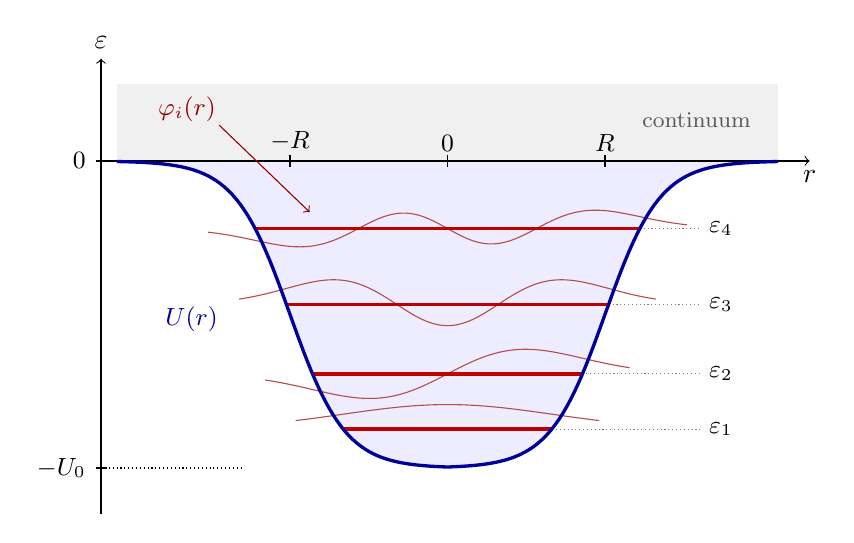
\begin{tikzpicture}[xscale=1.0,yscale=1.3,
  declare function={
    Uws(\x)=-3/(1+exp((abs(\x)-2)/0.35));
    phi(\t,\n)=ifthenelse(\n==0,1,ifthenelse(\n==1,1.65*\t,ifthenelse(\n==2,0.87*(2*\t*\t-1),0.55*(2*\t*\t*\t-3*\t))))*exp(-\t*\t/2);
  }]
  % continuum region
  \fill[gray!12] (-4.2,0) rectangle (4.2,0.75);
  \node[gray!70!black,font=\footnotesize,right] at (2.35,0.4) {continuum};
  % well interior
  \fill[blue!7] plot[domain=-4.2:4.2,samples=161] (\x,{Uws(\x)}) -- (4.2,0) -- (-4.2,0) -- cycle;
  % axes
  \draw[->] (-4.4,0) -- (4.6,0) node[below] {$r$};
  \draw[->] (-4.4,-3.45) -- (-4.4,1.0) node[above] {$\varepsilon$};
  \draw (-4.47,0) -- (-4.33,0) node[pos=0,left,font=\small] {$0$};
  \draw (-4.47,-3) -- (-4.33,-3) node[pos=0,left,font=\small] {$-U_0$};
  \draw[densely dotted] (-4.4,-3) -- (-2.6,-3);
  % nuclear radius
  \foreach \s in {-2,0,2} \draw (\s,0.06) -- (\s,-0.06);
  \node[above,font=\small] at (2,0) {$R$};
  \node[above,font=\small] at (-2,0) {$-R$};
  \node[above,font=\small] at (0,0) {$0$};
  % levels and wave functions
  \foreach \e/\n in {-2.62/0,-2.08/1,-1.40/2,-0.66/3}{
    \pgfmathsetmacro\xt{2+0.35*ln(3/(-\e)-1)}
    \pgfmathsetmacro\b{\xt/sqrt(2*\n+1)}
    \pgfmathsetmacro\lab{int(\n+1)}
    \draw[red!60!black!70,thin,smooth] plot[domain={-\xt-0.6}:{\xt+0.6},samples=90]
         (\x,{\e+0.24*phi(\x/\b,\n)});
    \draw[very thick,red!75!black] (-\xt,\e) -- (\xt,\e);
    \draw[densely dotted,gray] (\xt,\e) -- (3.2,\e);
    \node[right,font=\small] at (3.2,\e) {$\varepsilon_{\lab}$};
  }
  % well
  \draw[very thick,blue!60!black] plot[domain=-4.2:4.2,samples=161] (\x,{Uws(\x)});
  \node[blue!60!black,font=\small] at (-3.25,-1.55) {$U(r)$};
  \draw[<-,red!60!black] (-1.75,-0.5) -- (-2.9,0.35) node[above left,font=\small,inner sep=1pt] {$\varphi_i(r)$};
\end{tikzpicture}
\end{center}
The antisymmetric many-body wave function is
\[
\Phi(1,\dots,A)=\frac{1}{\sqrt{A!}}\sum_P(-1)^P\,\varphi_1(1)\varphi_2(2)\cdots\varphi_A(A)
\]
\[
=\frac{1}{\sqrt{A!}}\Big[\varphi_1(1)\varphi_2(2)\cdots\varphi_A(A)-\varphi_1(2)\varphi_2(1)\varphi_3(3)\cdots\varphi_A(A)+\dots\Big],
\]
where the sum runs over all permutations $P$ of particle indices. Equivalently,
\[
\Phi(1,2,\dots,A)=\frac{1}{\sqrt{A!}}
\begin{vmatrix}
\varphi_1(1)&\varphi_2(1)&\cdots&\varphi_A(1)\\
\varphi_1(2)&\varphi_2(2)&\cdots&\varphi_A(2)\\
\vdots&\vdots&\ddots&\vdots\\
\varphi_1(A)&\varphi_2(A)&\cdots&\varphi_A(A)
\end{vmatrix}
\qquad\text{(Slater determinant)}.
\]
If $\braket{\varphi_i|\varphi_j}=\delta_{ij}$, then $\braket{\Phi|\Phi}=1$.

In the ground state the nucleons fill the lowest levels of the mean-field potential $\op U$ up to the Fermi energy $\varepsilon_F$:
\begin{center}
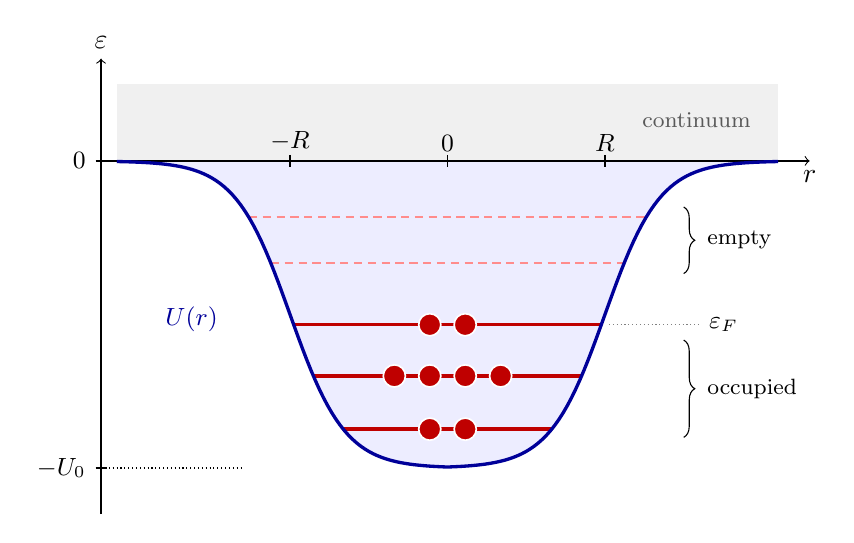
\begin{tikzpicture}[xscale=1.0,yscale=1.3,
  declare function={Uws(\x)=-3/(1+exp((abs(\x)-2)/0.35));},
  nucleon/.style={circle,fill=red!75!black,draw=white,line width=0.6pt,inner sep=0pt,minimum size=8pt}]
  % continuum region
  \fill[gray!12] (-4.2,0) rectangle (4.2,0.75);
  \node[gray!70!black,font=\footnotesize,right] at (2.35,0.4) {continuum};
  % well interior
  \fill[blue!7] plot[domain=-4.2:4.2,samples=161] (\x,{Uws(\x)}) -- (4.2,0) -- (-4.2,0) -- cycle;
  % axes
  \draw[->] (-4.4,0) -- (4.6,0) node[below] {$r$};
  \draw[->] (-4.4,-3.45) -- (-4.4,1.0) node[above] {$\varepsilon$};
  \draw (-4.47,0) -- (-4.33,0) node[pos=0,left,font=\small] {$0$};
  \draw (-4.47,-3) -- (-4.33,-3) node[pos=0,left,font=\small] {$-U_0$};
  \draw[densely dotted] (-4.4,-3) -- (-2.6,-3);
  \foreach \s in {-2,0,2} \draw (\s,0.06) -- (\s,-0.06);
  \node[above,font=\small] at (2,0) {$R$};
  \node[above,font=\small] at (-2,0) {$-R$};
  \node[above,font=\small] at (0,0) {$0$};
  % empty levels
  \foreach \e in {-1.0,-0.55}{
    \pgfmathsetmacro\xt{2+0.35*ln(3/(-\e)-1)}
    \draw[thick,red!45,densely dashed] (-\xt,\e) -- (\xt,\e);
  }
  % occupied levels: energy / number of nucleons
  \foreach \e/\N in {-2.62/2,-2.1/4,-1.6/2}{
    \pgfmathsetmacro\xt{2+0.35*ln(3/(-\e)-1)}
    \draw[very thick,red!75!black] (-\xt,\e) -- (\xt,\e);
    \foreach \k in {1,...,\N}
      \node[nucleon] at ({0.45*(\k-(\N+1)/2)},\e) {};
  }
  % Fermi energy
  \draw[densely dotted,gray] (2.05,-1.6) -- (3.2,-1.6) node[right,black,font=\small] {$\varepsilon_F$};
  % braces
  \draw[decorate,decoration={brace,amplitude=4pt}] (3.0,-0.45) -- (3.0,-1.1)
     node[midway,right=5pt,font=\footnotesize,align=left] {empty};
  \draw[decorate,decoration={brace,amplitude=4pt}] (3.0,-1.75) -- (3.0,-2.7)
     node[midway,right=5pt,font=\footnotesize,align=left] {occupied};
  % well
  \draw[very thick,blue!60!black] plot[domain=-4.2:4.2,samples=161] (\x,{Uws(\x)});
  \node[blue!60!black,font=\small] at (-3.25,-1.55) {$U(r)$};
\end{tikzpicture}
\end{center}

\subsection{Experimental evidence for a mean field}
The experimental evidence for a mean field is the \textbf{shell structure} of nuclei: there are ``magic'' numbers similar to atomic systems.

%--- magic-number plots ---
Two particularly clear signatures of shell closures are shown in Figs.~\ref{fig:S2n} and~\ref{fig:E2plus}. The two-neutron and two-proton separation energies
\[
S_{2n}(A,Z)=B(A,Z)-B(A-2,Z),\qquad S_{2p}(A,Z)=B(A,Z)-B(A-2,Z-2)
\]
are the energies needed to remove two neutrons (protons) from the nucleus; removing a \emph{pair} of nucleons eliminates the odd-even staggering caused by pairing. Along an isotopic chain $S_{2n}$ decreases smoothly with increasing $N$, as expected from the liquid-drop (Bethe--Weizs\"acker) formula, but it drops abruptly just after $N=28,50,82,126$: the two neutrons added beyond a closed shell have to occupy the next, considerably less bound shell. The same behaviour of $S_{2p}$ is seen after $Z=50$ and $Z=82$.

\begin{figure}[htbp]
    \centering
    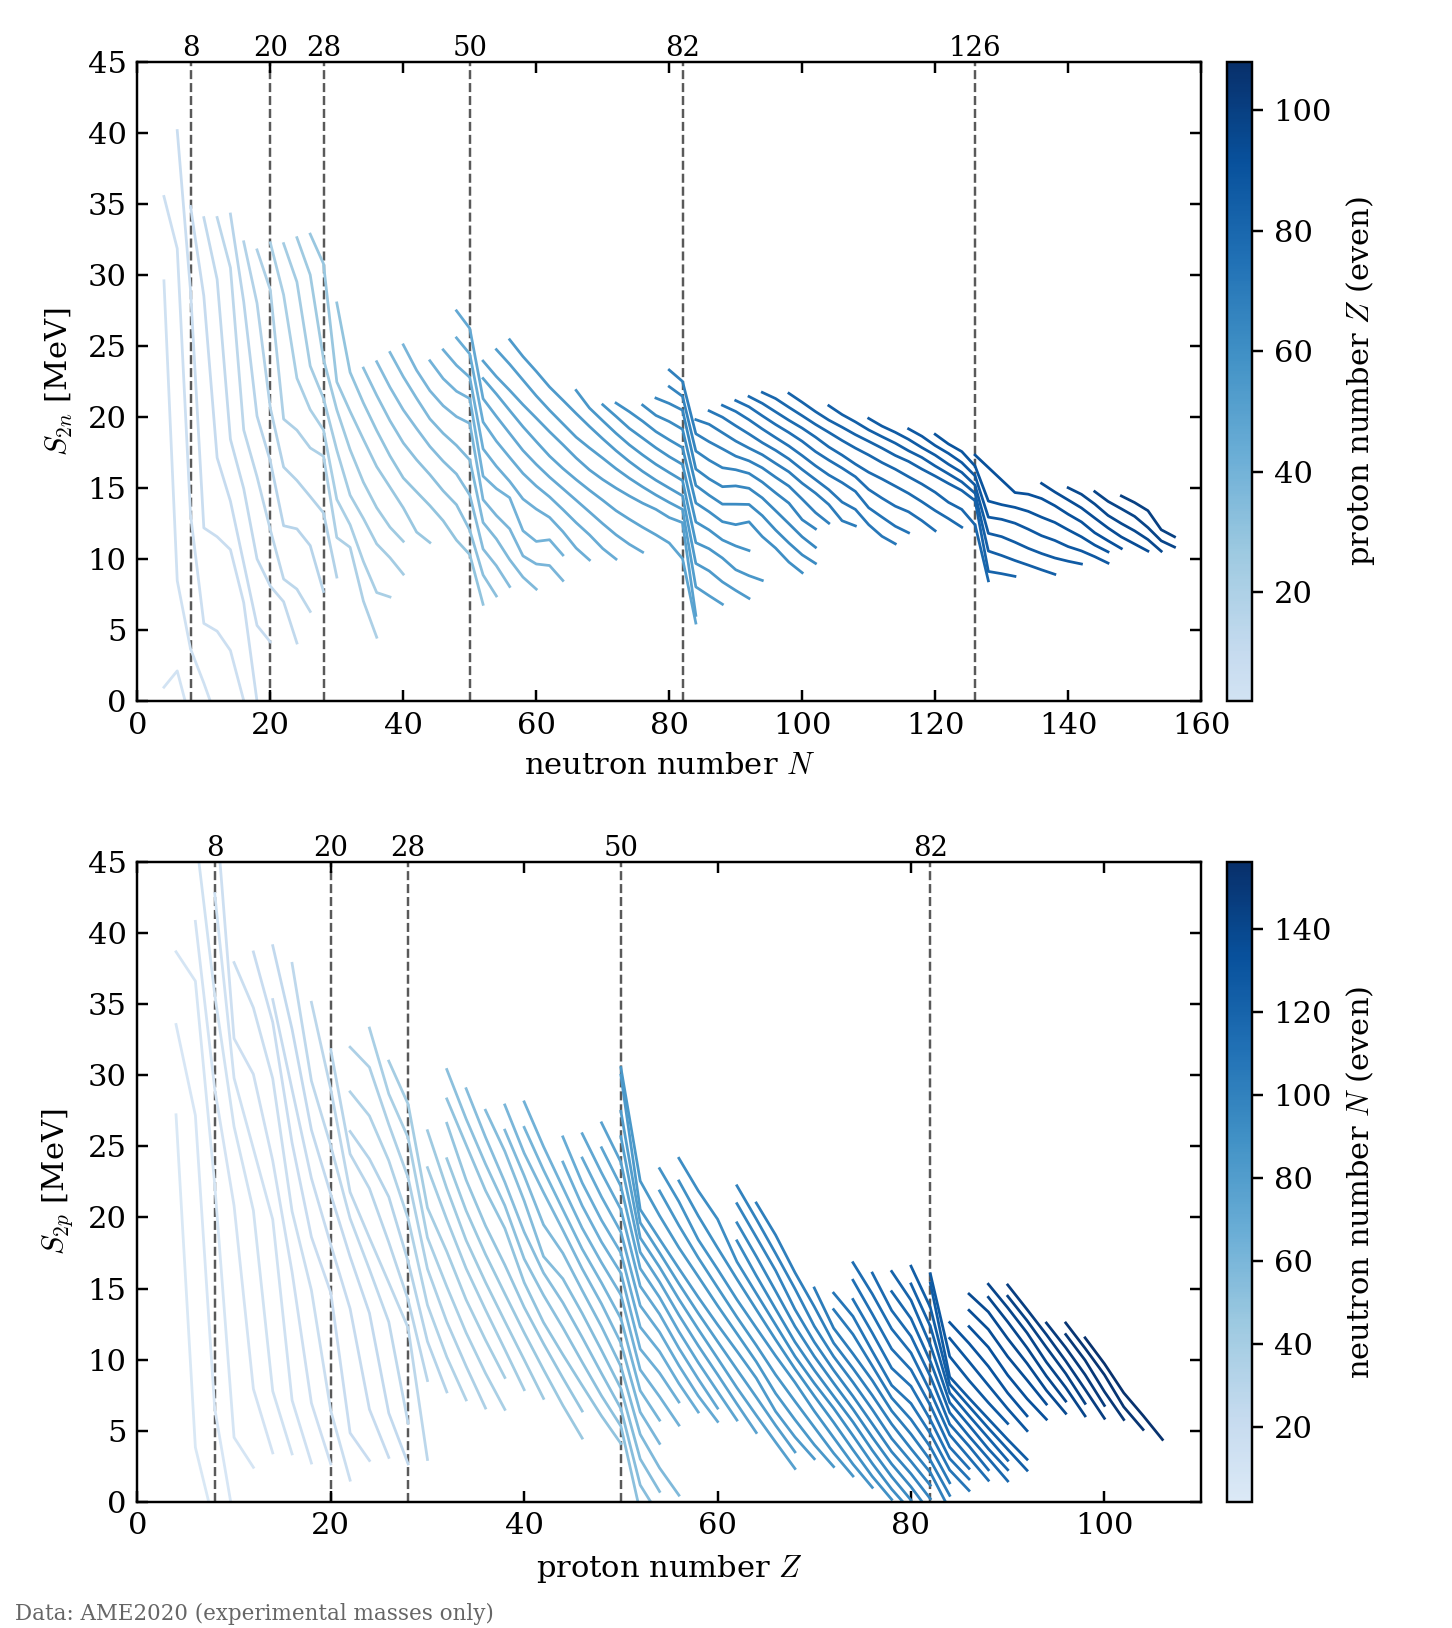
\includegraphics[width=0.85\linewidth]{s2n_s2p.png}
    \caption{Two-neutron separation energies $S_{2n}$ along isotopic chains (top) and two-proton separation energies $S_{2p}$ along isotonic chains (bottom) for even-even nuclei. Dashed lines mark the magic numbers. Data: AME2020 atomic mass evaluation (experimental masses only).}
    \label{fig:S2n}
\end{figure}

The energy of the first excited $2^+$ state in even-even nuclei (Fig.~\ref{fig:E2plus}) shows an even more striking pattern. In most nuclei $E(2^+_1)$ lies well below $1$~MeV, and far from closed shells (rare earths, actinides) it decreases to $\sim 100$~keV and below --- these are the collective rotational states discussed in Sec.~\ref{sec:rot}. For a magic number of protons or neutrons, however, $E(2^+_1)$ shows sharp peaks, and in the doubly magic nuclei $^{16}$O, $^{40}$Ca, $^{48}$Ca, $^{132}$Sn and $^{208}$Pb it reaches $3$--$7$~MeV: to excite such a nucleus a nucleon has to be promoted across the shell gap. Far from stability the shell structure may change: e.g.\ $^{32}$Mg ($N=20$) has a low-lying $2^+$ state (the $N=20$ shell closure disappears in the ``island of inversion''), whereas $^{24}$O shows a high $2^+$ state signalling a new shell closure at $N=16$.

\begin{figure}[htbp]
    \centering
    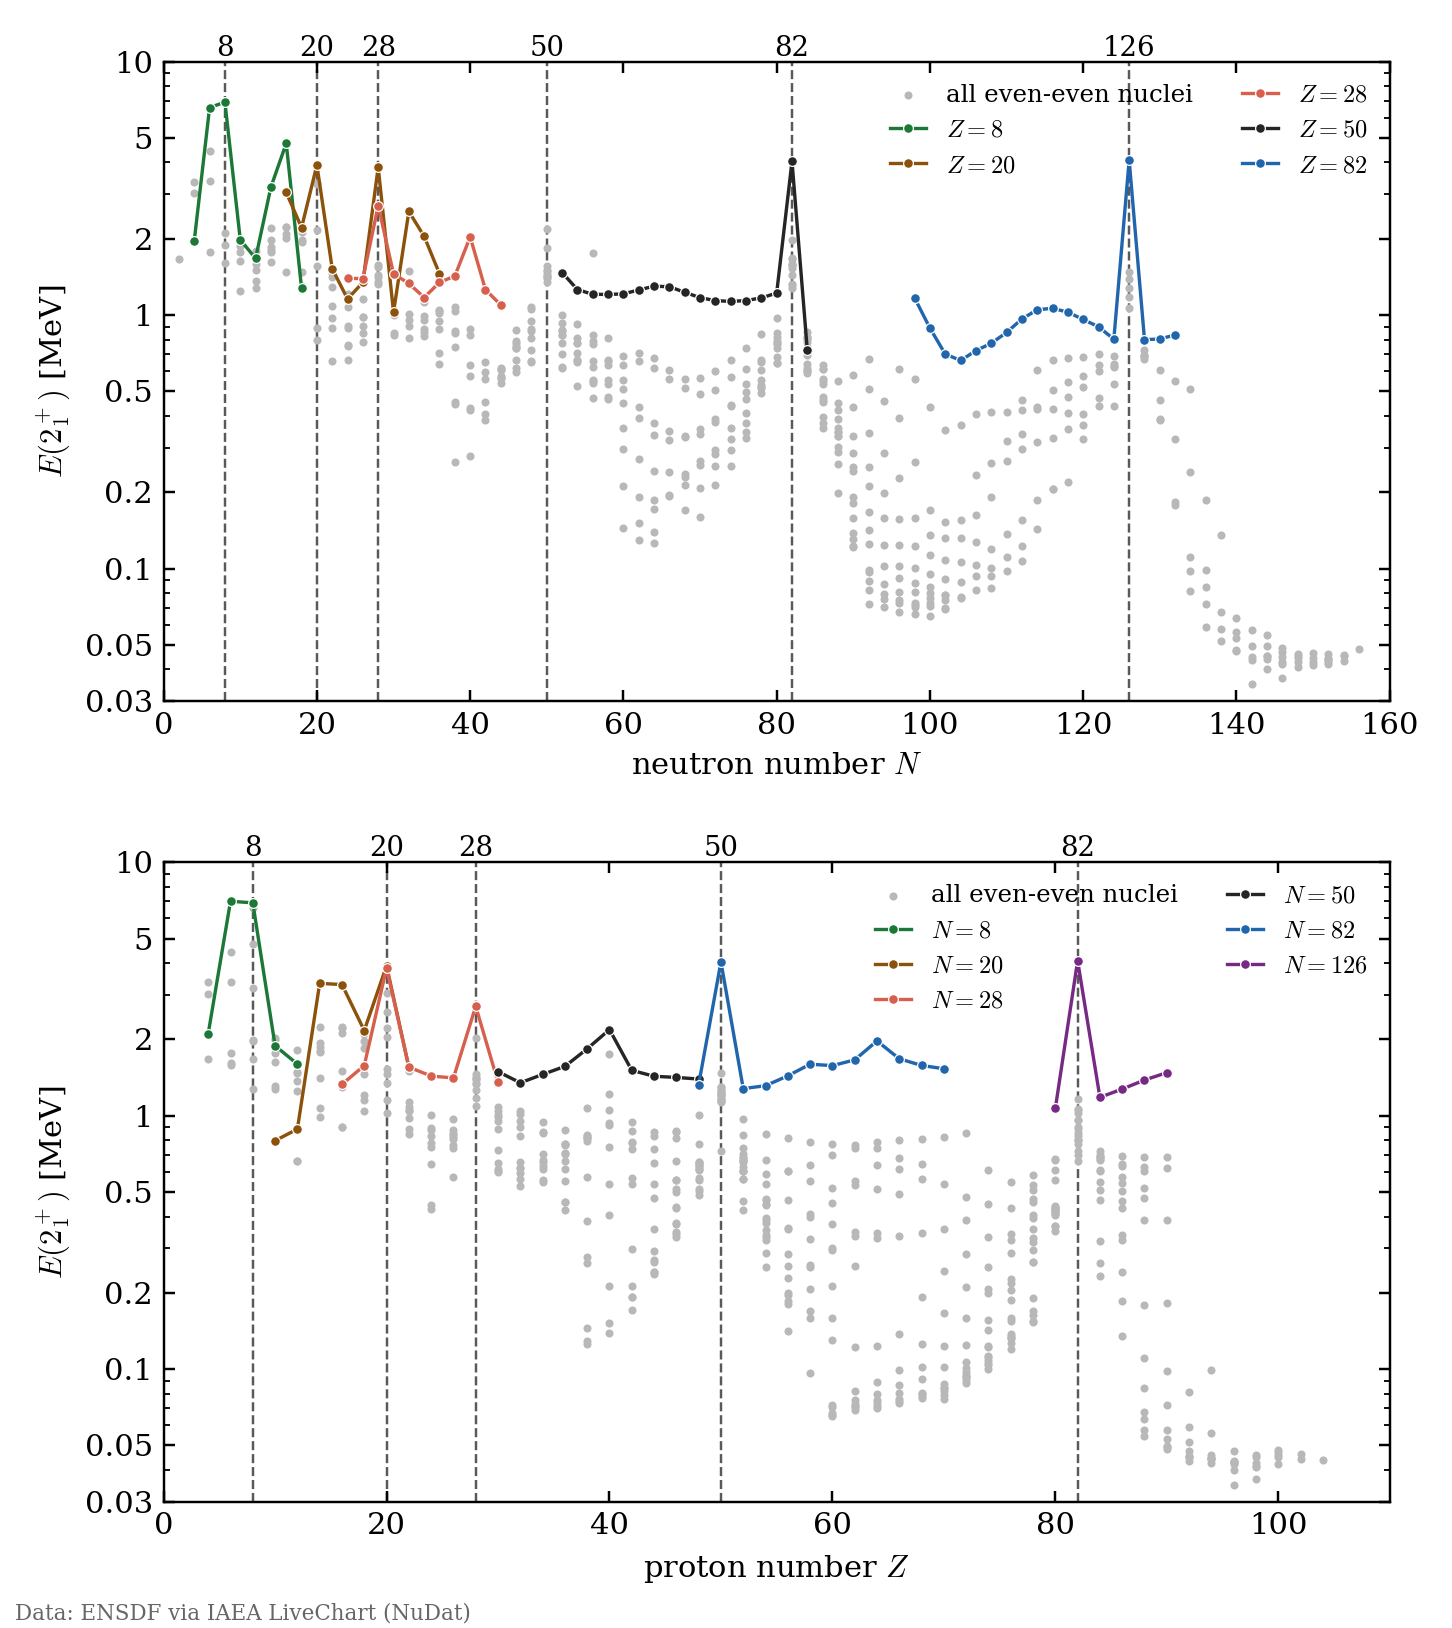
\includegraphics[width=0.85\linewidth]{e2plus.png}
    \caption{Excitation energy of the first $2^+$ state in even-even nuclei as a function of the neutron number (top) and proton number (bottom), logarithmic scale. Grey points: all even-even nuclei; coloured lines: chains with a magic number of protons (top) or neutrons (bottom). Data: ENSDF, retrieved via the IAEA LiveChart of Nuclides (same data as NuDat).}
    \label{fig:E2plus}
\end{figure}

Reminder: solutions of the Schr\"odinger equation for a spherical potential $U(r)$,
\[
\Big[-\frac{\hbar^2}{2m}\Delta+U\Big]\varphi_{n\ell}=E_{n\ell}\,\varphi_{n\ell},
\qquad
\Delta=\frac{\partial^2}{\partial r^2}+\frac2r\frac{\partial}{\partial r}-\frac{\op{\vec\ell}^{\,2}}{\hbar^2r^2}.
\]
In spherical coordinates
\[
\varphi_{n\ell m}=R_{n\ell}(r)\,Y_{\ell m}(\vartheta,\varphi),
\]
and the radial equation reads
\[
\Big[\frac{\ud^2}{\ud r^2}+\frac2r\frac{\ud}{\ud r}-\frac{\ell(\ell+1)}{r^2}+\frac{2m}{\hbar^2}\big(E_{n\ell}-U\big)\Big]R_{n\ell}=0,
\]
with
\[
\op{\vec\ell}^{\,2}\,Y_{\ell m}(\vartheta,\varphi)=\hbar^2\ell(\ell+1)\,Y_{\ell m}(\vartheta,\varphi),
\qquad \ell=0,1,2,\dots,\quad m=-\ell,\dots,0,\dots,\ell .
\]

\subsubsection*{Infinite square well}
\[
U(r)=\begin{cases}-U_0, & r\le R,\\ \infty, & r>R,\end{cases}
\]
\begin{center}
\begin{tikzpicture}[scale=0.8]
\draw[->] (-0.3,0) -- (3.5,0) node[right]{$r$};
\draw[->] (0,-2.3) -- (0,1.0);
\draw[thick] (0,-1.8) -- (2,-1.8) -- (2,1.0);
\node[above right] at (2,0) {$R$};
\node[right] at (2,-1.8) {$-U_0$};
\node[above] at (2,1.0) {$\infty$};
\end{tikzpicture}
\end{center}
The regular solution inside the well is given by spherical Bessel functions $j_\ell$,
\[
R_{n\ell}(r)=N_{n\ell}\,j_\ell(k_{n\ell}r),
\qquad
k_{n\ell}^2=\frac{2m}{\hbar^2}\big(E_{n\ell}+U_0\big).
\]
The boundary condition
\[
R_{n\ell}(R)\overset{!}{=}0\quad\Longrightarrow\quad j_\ell(k_{n\ell}R)\overset{!}{=}0
\quad\Longrightarrow\quad k_{n\ell}R\ \text{is a root of } j_\ell ,
\qquad
E_{n\ell}=\frac{\hbar^2}{2m}k_{n\ell}^2-U_0 .
\]
Eigenstates:
\[
\begin{array}{llll}
\ell=0: & j_0(k_{n0}R)\overset{!}{=}0, & k_{10}R=\pi,\ \ k_{20}R=2\pi,\ \ k_{30}R=3\pi, & E_{10},E_{20},E_{30}\ \to\ 1s,2s,3s,\\[1mm]
\ell=1: & j_1(k_{n1}R)\overset{!}{=}0, & k_{11}R=4.49,\ \ k_{21}R=7.72,\ \ k_{31}R=10.9, & E_{11},E_{21},E_{31}\ \to\ 1p,2p,3p,\\[1mm]
\ell=2: & j_2(k_{n2}R)\overset{!}{=}0, & & E_{12},E_{22},E_{32}\ \to\ 1d,2d,3d,
\end{array}
\]
where $E_{10}=\frac{\hbar^2}{2m}k_{10}^2-U_0$, etc.
The wave functions are
\[
\varphi_{n\ell m}(r,\vartheta,\varphi)=N_{n\ell}\,j_\ell(k_{n\ell}r)\,Y_{\ell m}(\vartheta,\varphi),
\]
\[
n=1,2,\dots,\quad \ell=0,1,2,\dots,\quad m=-\ell,\dots,\ell,
\]
with $k_{n\ell}R$ the $n$-th root of $j_\ell$.

\subsubsection*{Harmonic oscillator}
\[
U(r)=\tfrac12 m\omega^2r^2-U_0 ,
\]
\[
R_{n\ell}(r)=N_{n\ell}\,(\nu r)^\ell\,e^{-\nu^2r^2/2}\,L_{n-1}^{\ell+1/2}(\nu^2r^2),
\qquad \nu=\sqrt{\frac{m\omega}{\hbar}},
\]
where $L_{n}^{\alpha}$ are the associated Laguerre polynomials. The energies are
\[
E_{n\ell}=\hbar\omega\Big(N+\frac32\Big)-U_0,
\qquad N=2(n-1)+\ell,\quad N=0,1,2,\dots
\]
where $N$ is the principal quantum number and $n=1,2,\dots$ the radial quantum number. The levels are equidistant ($0\hbar\omega$, $1\hbar\omega$, $2\hbar\omega$, \dots) and the parity of a state is $(-1)^\ell$, because
$Y_{\ell m}(\pi-\vartheta,\varphi+\pi)=(-1)^\ell\,Y_{\ell m}(\vartheta,\varphi)$.
\begin{center}
\begin{tabular}{c c c c l c}
$N$ & $n$ & $\ell$ & & shell & parity \\ \hline
0 & 1 & 0 & $1s$ & $s$-shell & $+$ \\ \hline
1 & 1 & 1 & $1p$ & $p$-shell & $-$ \\ \hline
2 & 2 & 0 & $2s$ & $sd$-shell & $+$ \\
  & 1 & 2 & $1d$ &  & $+$ \\ \hline
3 & 2 & 1 & $2p$ & $pf$-shell & $-$ \\
  & 1 & 3 & $1f$ &  & $-$ \\ \hline
4 & 3 & 0 & $3s$ & & $+$ \\
  & 2 & 2 & $2d$ & $sdg$-shell & $+$ \\
  & 1 & 4 & $1g$ & & $+$ \\ \hline
\end{tabular}
\end{center}

%--- radial wave functions plot ---
\paragraph{Radial wave functions.} The lowest radial wave functions $R_{n\ell}(r)$ of the infinite square well and of the harmonic oscillator, normalized as $\int_0^\infty R_{n\ell}^2(r)\,r^2\,\ud r=1$, are compared in Fig.~\ref{fig:radial}. In both cases $R_{n\ell}$ has $n-1$ nodes for $0<r<R$ (square well) or $0<r<\infty$ (HO), and close to the origin $R_{n\ell}\sim r^\ell$: the centrifugal term $\ell(\ell+1)/r^2$ pushes the states with higher $\ell$ outwards, and only the $s$-states are nonzero at $r=0$. The two potentials differ at the surface: in the infinite well the wave function is forced to vanish at $r=R$, whereas the HO wave functions decay smoothly as $e^{-\nu^2r^2/2}$ beyond the classical turning point. A realistic nuclear potential (Woods--Saxon, below) lies between these two limits; the middle row of Fig.~\ref{fig:radial} shows its radial functions for $A=208$ ($V_0=50$~MeV, $R_{\rm WS}=1.27\,A^{1/3}=7.5$~fm, $a=0.67$~fm, no spin-orbit term, obtained numerically). Inside the nucleus they resemble the square-well functions, since the potential is nearly flat there, but the surface is diffuse: the wave function does not vanish at $R_{\rm WS}$ and decays exponentially outside, $u_{n\ell}\sim e^{-\kappa r}$ with $\kappa=\sqrt{2m|\varepsilon_{n\ell}|}/\hbar$. The tail is longer for less bound states, e.g.\ the $3d$ state with $\varepsilon\approx-5$~MeV extends well beyond the nuclear surface, whereas the deeply bound $1s$ state ($\varepsilon\approx-46$~MeV) is confined to the interior.

\begin{figure}[htbp]
    \centering
    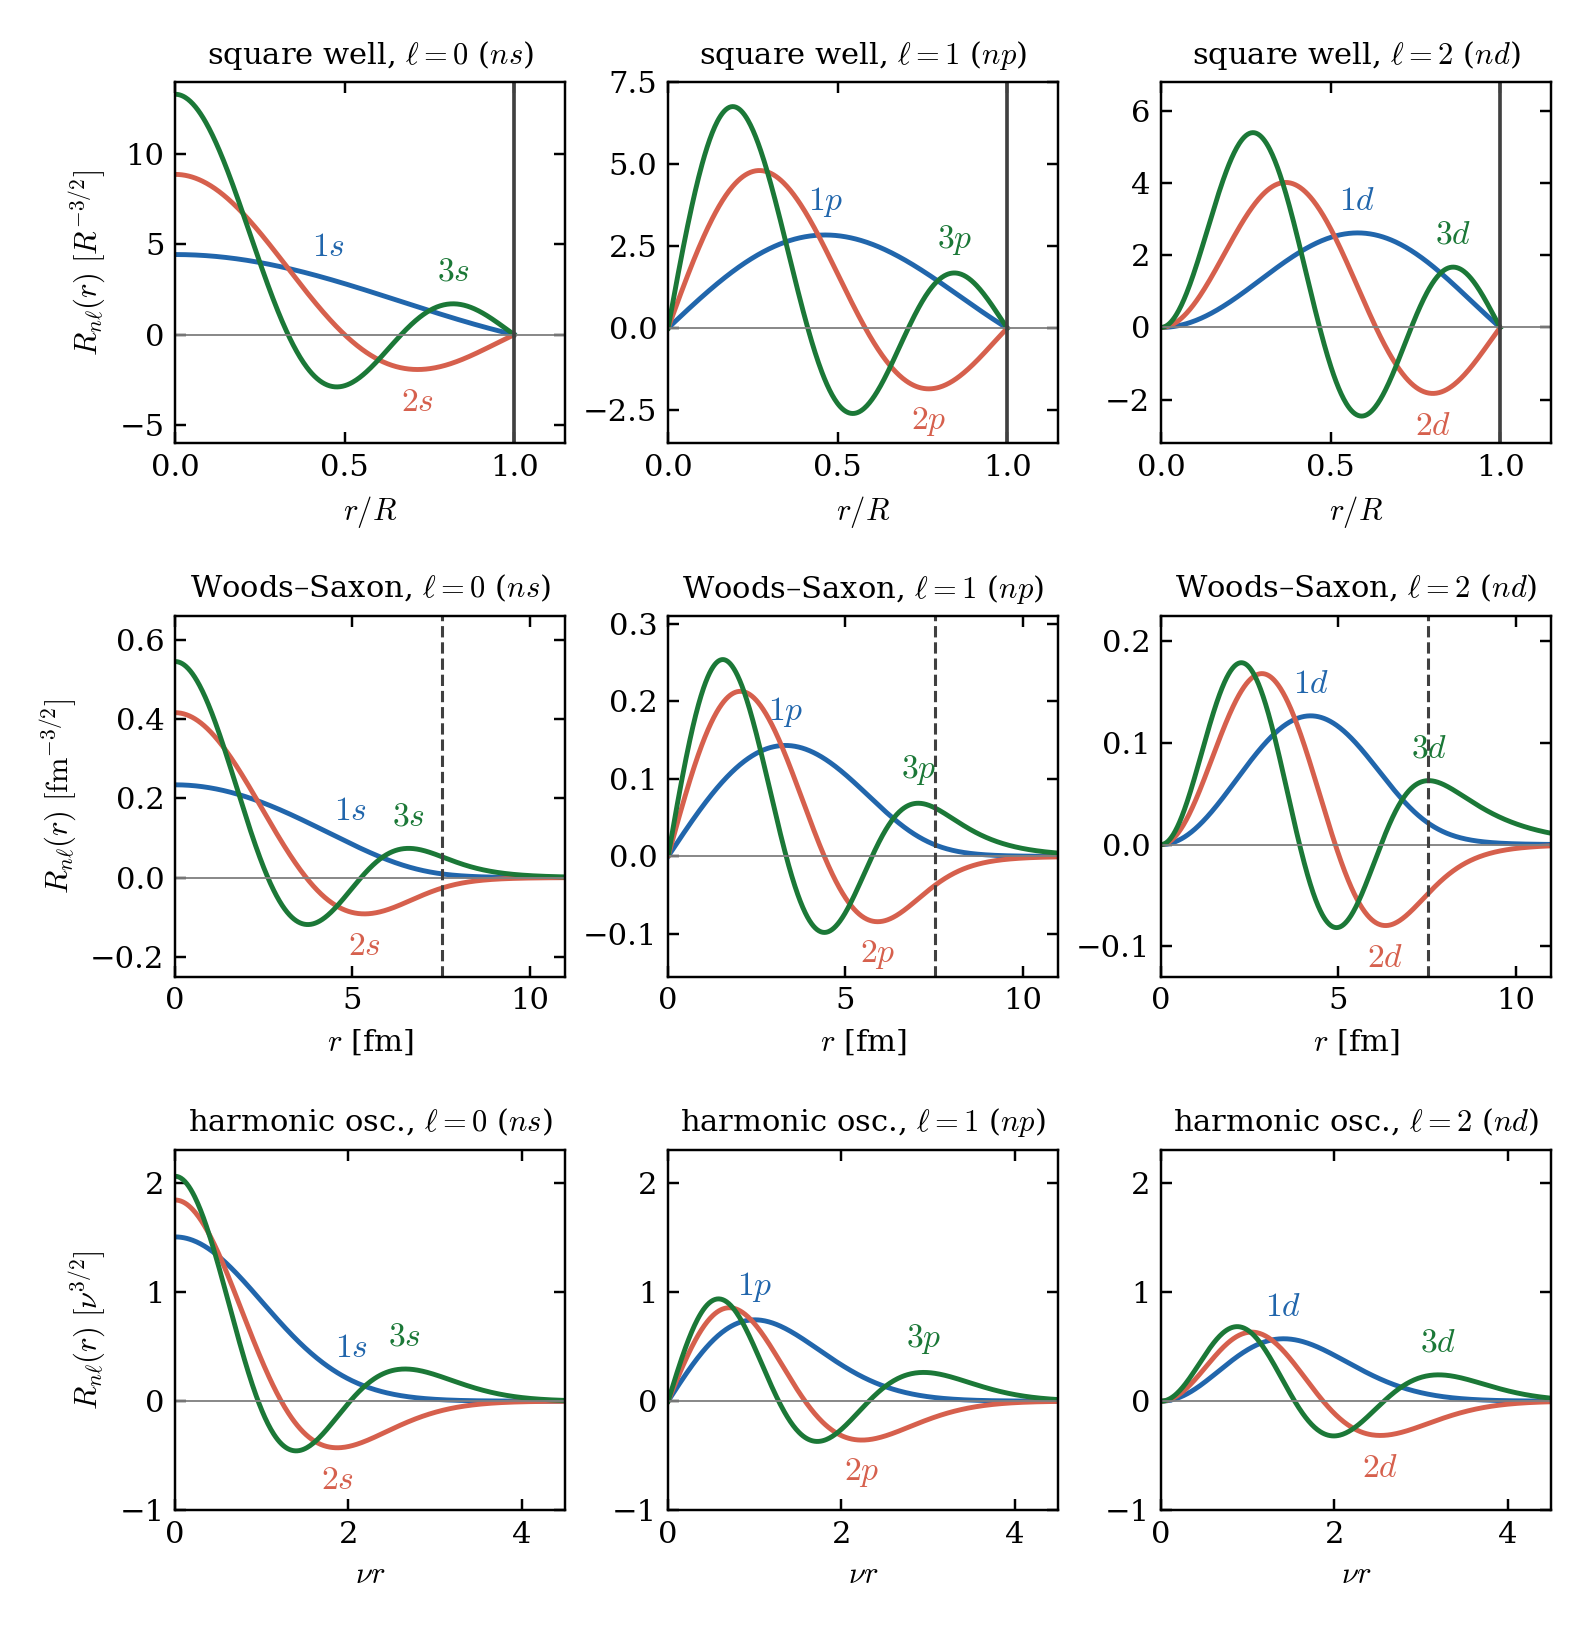
\includegraphics[width=1.0\linewidth]{radial_wf.png}
    \caption{Radial wave functions $R_{n\ell}(r)$ with $n=1,2,3$ and $\ell=0,1,2$ for the infinite square well of radius $R$ (top, in units of $R^{-3/2}$), for the Woods--Saxon potential with $A=208$, $V_0=50$~MeV, $a=0.67$~fm (middle, in fm$^{-3/2}$; the dashed line marks $R_{\rm WS}=7.5$~fm) and for the harmonic oscillator (bottom, in units of $\nu^{3/2}$, $\nu=\sqrt{m\omega/\hbar}$).}
    \label{fig:radial}
\end{figure}

%--- density profiles plot ---
\paragraph{Density profiles.} The density of $Z$ protons occupying the lowest orbits is obtained by summing the contributions of all occupied single-particle states,
\[
\rho_p(r)=\sum_{i\in\text{occ}}|\varphi_i(\vec r)|^2=\frac{1}{4\pi}\sum_{n\ell j\in\text{occ}}(2j+1)\,R_{n\ell}^2(r),
\]
where we used $\sum_m|Y_{\ell m}|^2=(2\ell+1)/4\pi$ and the factor $2j+1$ counts the states of a filled $j$-orbit. Figure~\ref{fig:density} shows the proton densities for $Z=8,20,28,50,82,126$ in the harmonic oscillator, in the infinite square well and in a Woods--Saxon potential (introduced below). The orbits are filled in the realistic order including the spin-orbit splitting (see below), so that all six cases have closed orbits and spherical densities; the radial functions depend only on $n,\ell$. Each panel corresponds to a nucleus with this magic proton number: $^{16}$O, $^{40}$Ca, $^{58}$Ni, $^{116}$Sn, $^{208}$Pb, and the hypothetical superheavy nucleus with $Z=126$, $N=184$ ($A=310$). The potentials are scaled with the actual mass number, $R=r_0A^{1/3}$, $r_0=1.2$~fm, and the Coulomb potential is neglected. The densities are normalized to $\int\rho_p\,\ud^3r=Z$. The parameters $\hbar\omega$ and $R_{\rm sw}$ are fixed by requiring that the mean square radius equals that of a uniform sphere of radius $R$, $\braket{r^2}=\frac35R^2$. For the HO,
\[
\braket{r^2}=\frac{1}{Z}\frac{\hbar}{m\omega}\sum_{n\ell j\in\text{occ}}(2j+1)\Big(N+\frac32\Big),
\qquad N=2(n-1)+\ell,
\]
which gives $\hbar\omega=17.0$~MeV ($^{16}$O), $12.3$~MeV ($^{40}$Ca), \dots, $6.6$~MeV ($^{208}$Pb), close to the empirical estimate $\hbar\omega\approx41A^{-1/3}$~MeV. The dashed line marks the equivalent sharp radius $R_{\rm eq}=\sqrt{\frac53\braket{r^2}_{\rm HO}}=R$. The Woods--Saxon potential is not rescaled: it has the typical parameters $V_0=50$~MeV, $R_{\rm WS}=1.27\,A^{1/3}$~fm, $a=0.67$~fm, and its eigenfunctions are obtained numerically.

All densities oscillate in the interior, reflecting the shell structure (e.g.\ the central dip for $^{16}$O, where only the $1s$ orbit contributes at $r=0$). The HO density is too large in the centre and has a long Gaussian tail, whereas the square-well density is cut off sharply at $r=R_{\rm sw}$. Neither reproduces the measured charge densities (open circles), obtained from elastic electron scattering (H.~de Vries, C.~W.~de Jager, C.~de Vries, At.\ Data Nucl.\ Data Tables \textbf{36} (1987) 495). These are approximately constant in the interior (saturation), $\rho_{\rm ch}(0)\approx0.065$--$0.085$~fm$^{-3}$, decreasing slowly with $A$ as $Z/A$ decreases, and have a diffuse surface of thickness $\approx2$--$2.5$~fm. The charge density is also normalized to $Z$, so it can be compared directly with $\rho_p$. It differs from the point-proton density only by folding with the charge distribution of the proton itself (rms radius $r_p\approx0.84$~fm), which slightly smears the surface; to a good approximation $\braket{r^2}_{\rm ch}=\braket{r^2}_p+r_p^2$. The Woods--Saxon density, obtained without any adjustment, lies between the two limits: its interior is flatter and its surface falls off smoothly. It follows the measured densities closely, especially in the surface region, and its rms radius agrees with the point-proton rms radius extracted from the data: $2.61$ vs.\ $2.60$~fm for $^{16}$O, $3.32$ vs.\ $3.35$~fm for $^{40}$Ca, and $5.39$ vs.\ $5.44$~fm for $^{208}$Pb. The remaining differences in the interior reflect the simplicity of the potential (no spin-orbit or Coulomb term). This is why the Woods--Saxon shape, discussed below, is used as a realistic phenomenological mean field.

\begin{figure}[htbp]
    \centering
    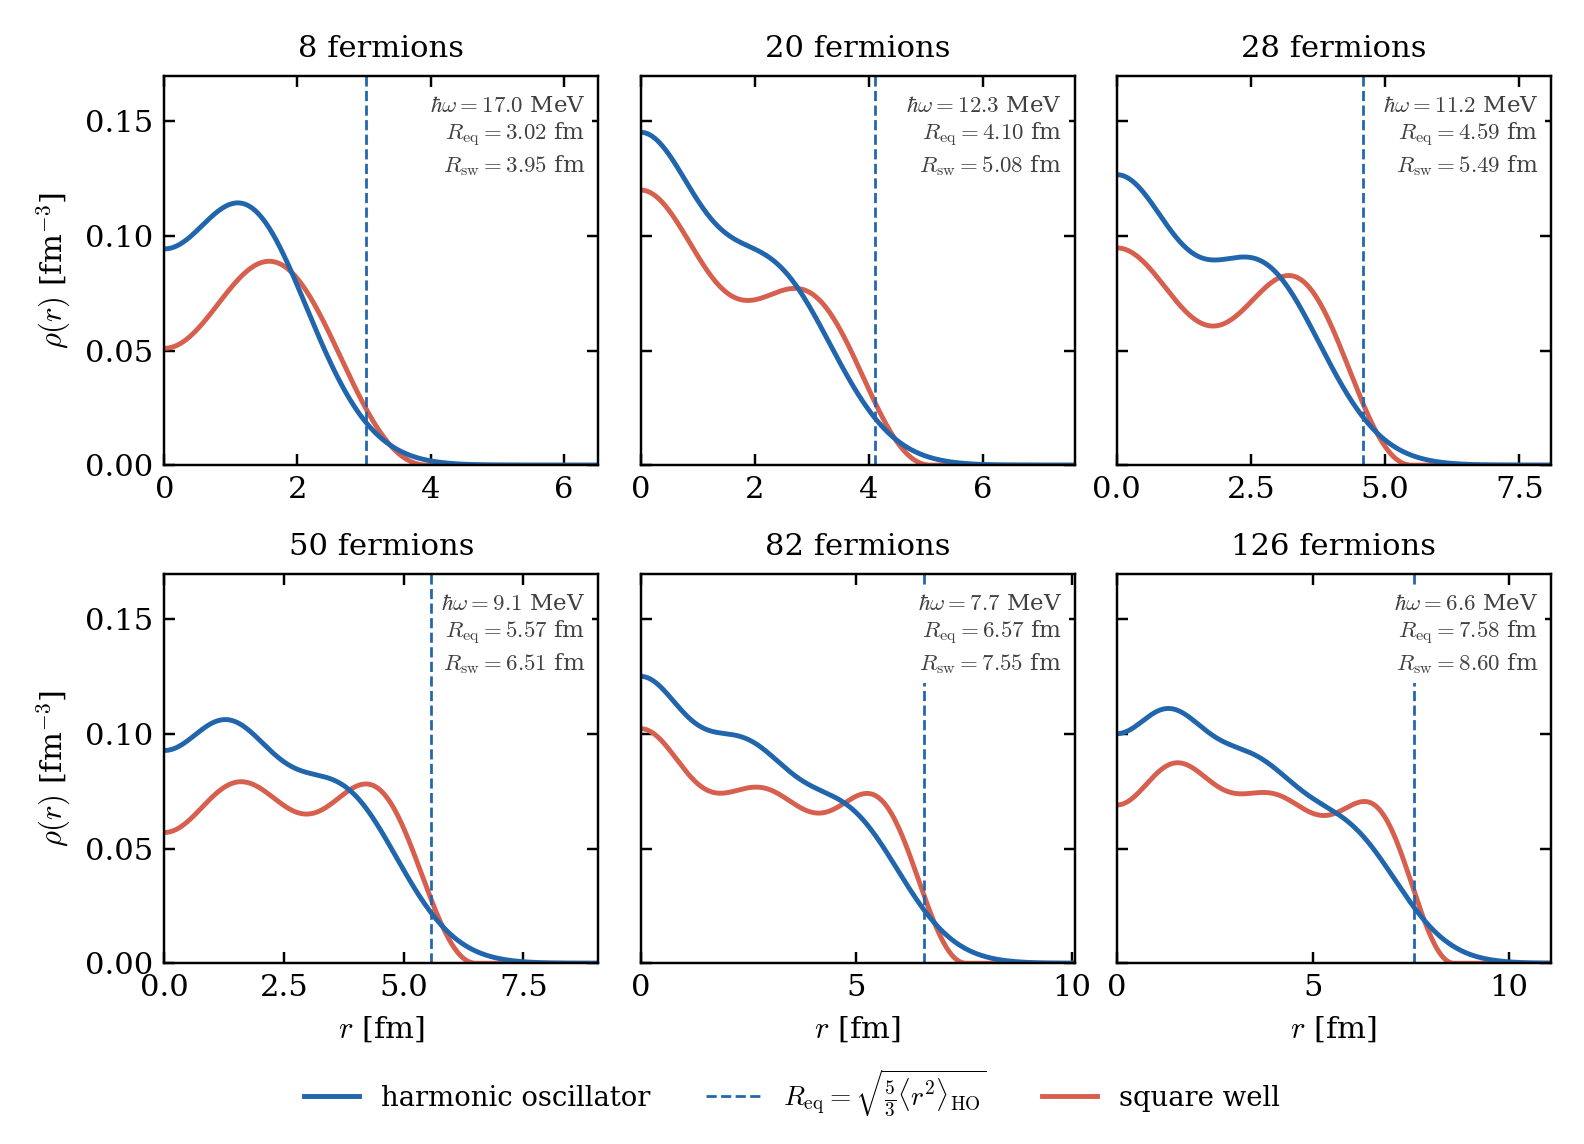
\includegraphics[width=1.0\linewidth]{density_profiles.png}
    \caption{Proton densities $\rho_p(r)$, normalized to $Z$, for $Z=8$, $20$, $28$, $50$, $82$, $126$ protons, corresponding to $^{16}$O, $^{40}$Ca, $^{58}$Ni, $^{116}$Sn, $^{208}$Pb and the hypothetical $^{310}126$ ($N=184$). Model densities: harmonic oscillator (blue), Woods--Saxon potential (green; $V_0=50$~MeV, $R_{\rm WS}=1.27\,A^{1/3}$~fm, $a=0.67$~fm) and infinite square well (red). For the HO and the square well, $\hbar\omega$ and $R_{\rm sw}$ are fixed by $\braket{r^2}=\frac35R^2$, $R=1.2\,A^{1/3}$~fm. Orbits are filled in the spin-orbit order ($1s_{1/2}$, $1p_{3/2}$, $1p_{1/2}$, $1d_{5/2}$, \dots). The dashed line is the equivalent sharp radius $R_{\rm eq}=\sqrt{5\braket{r^2}_{\rm HO}/3}$. Open circles: measured charge densities from elastic electron scattering (Fourier--Bessel fits, sum of Gaussians for $^{116}$Sn; de Vries et al.\ 1987); no data exist for $Z=126$.}
    \label{fig:density}
\end{figure}

\paragraph{Degeneracy of HO shells.} For a major shell $N$ we have $\ell=N-2(n-1)$, i.e.\ $2\ell+1=2N-4n+5$. Including the factor 2 for spin:

$N$ even ($n=1,\dots,N/2+1$):
\[
d_N=2\sum_{n=1}^{N/2+1}(2N-4n+5)
=4N\Big(\frac N2+1\Big)-8\,\frac{\frac N2+1}{2}\Big(\frac N2+2\Big)+10\Big(\frac N2+1\Big)
\]
\[
=\Big(\frac N2+1\Big)(4N-2N-8+10)=(N+1)(N+2).
\]
$N$ odd ($n=1,\dots,(N+1)/2$):
\[
d_N=2\sum_{n=1}^{(N+1)/2}(2N-4n+5)
=4N\,\frac{N+1}{2}-8\,\frac{N+1}{4}\Big(\frac{N+1}{2}+1\Big)+10\,\frac{N+1}{2}
\]
\[
=(N+1)(2N-N-1-2+5)=(N+1)(N+2).
\]
Thus $d_0=2$, $d_1=6$, $d_2=12$, $d_3=20$, $d_4=30$, $d_5=42$. For completely filled shells $0,\dots,N$ we get the total numbers of particles
\[
\begin{array}{ll}
N=0: & 2,\\
N=1: & 8=6+2,\\
N=2: & 20=12+8,\\
N=3: & 40=20+20,\\
N=4: & 70=30+40,\\
N=5: & 112=42+70.
\end{array}
\]
Magic numbers
\begin{itemize}
\item for the harmonic oscillator: $2,8,20,40,70,112,\dots$
\item for the (infinite) square well: $2,8,20,34,58,92,\dots$
\end{itemize}

\subsubsection*{``Realistic'' case: Woods--Saxon potential}
\[
U(r)=-\frac{V_0}{1+e^{(r-R)/a}}
\]
\begin{center}
\begin{tikzpicture}[xscale=0.6,yscale=0.8]
\draw[->] (-0.3,0) -- (6,0) node[right]{$r$};
\draw[->] (0,-2.3) -- (0,0.8);
\draw[thick,domain=0:5.6,samples=100,smooth] plot (\x,{-2/(1+exp((\x-3)/0.4))});
\draw (3,0.08) -- (3,-0.08) node[above=3pt]{$R$};
\node[left] at (0,-2) {$-V_0$};
\end{tikzpicture}
\end{center}
The Woods--Saxon potential alone cannot reproduce the observed shells either.

%--- single-particle spectra plot ---
This is illustrated in Fig.~\ref{fig:spspectra}, which compares the single-particle spectra (without spin-orbit term) of the harmonic oscillator, of a Woods--Saxon potential with typical parameters of a heavy nucleus ($V_0=50$~MeV, $R=1.27\,A^{1/3}$~fm, $a=0.67$~fm, $A=208$), and of the infinite square well. To make the spectra comparable, each of them is shifted so that $E_{1s}=0$ and scaled by a single factor fitted to the HO shell energies. Going from the HO to the square well, the degeneracy of the HO major shells is lifted and in each shell the state with the largest $\ell$ ($1d$, $1f$, $1g$, $1h$, $1i$) is lowered most: these states are localized at large $r$ (cf.\ Fig.~\ref{fig:radial}), where the flat-bottomed potentials are deeper than the HO. The magic numbers $2,8,20$ appear for all three potentials, but none of them reproduces the observed magic numbers $28,50,82,126$ --- the gaps appear at $34,40,58,92,138$ instead. An additional ingredient is needed: the spin-orbit interaction.

\begin{figure}[htbp]
    \centering
    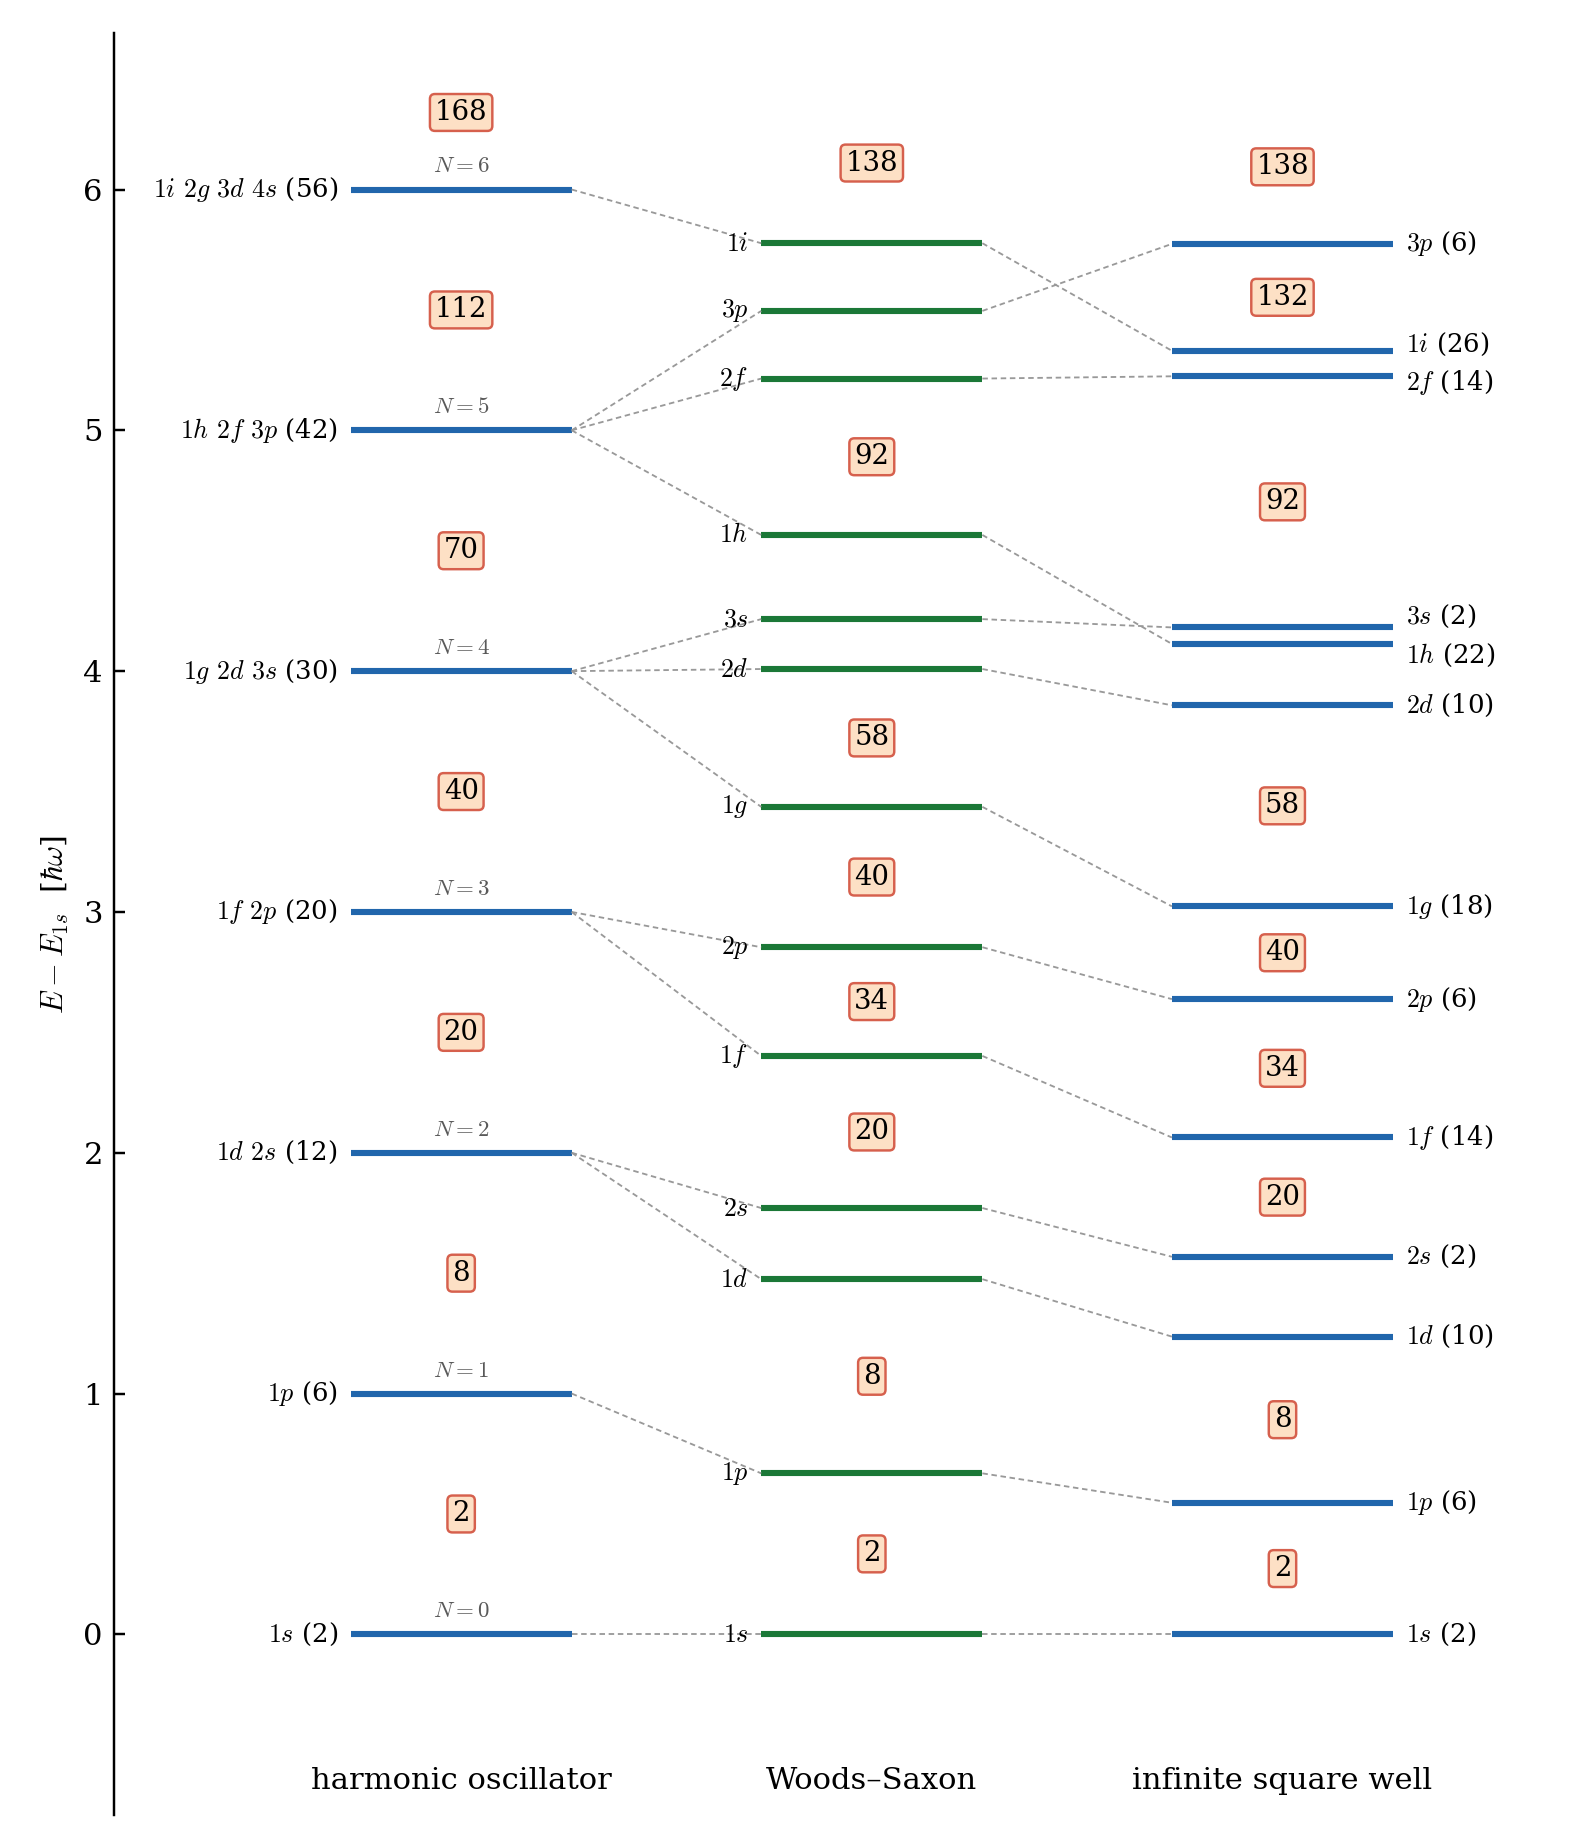
\includegraphics[width=0.85\linewidth]{sp_spectra.png}
    \caption{Single-particle spectra without spin-orbit term: harmonic oscillator (left), Woods--Saxon potential with $V_0=50$~MeV, $R=7.52$~fm, $a=0.67$~fm (middle), and infinite square well (right). Each spectrum is shifted so that $E_{1s}=0$ and scaled to the HO shell energies (units of $\hbar\omega$). Numbers in brackets are the degeneracies $2(2\ell+1)$ (HO: of the whole shell); boxed numbers give the total number of particles below gaps larger than $0.38\,\hbar\omega$. Dashed lines connect the same $n\ell$ states.}
    \label{fig:spspectra}
\end{figure}

%--- single-particle evolution with A ---
\paragraph{Evolution with the mass number.} How the single-particle spectrum changes from light to heavy nuclei is shown in Fig.~\ref{fig:spevolA}. The neutron and proton levels are computed for nuclei on the $\beta$-stability line, $A=4$--$270$, with a realistic Woods--Saxon potential. The potential already includes the Coulomb term for protons and the spin-orbit term discussed in the next subsection (``Seminole'' parametrization, M.~Schwierz, I.~Wiedenh\"over, A.~Volya, arXiv:0709.3525). Several features are general:
\begin{itemize}
\item As $A$ grows, the well becomes wider and all levels go down, roughly as $A^{-2/3}$ (cf.\ the square well, $E\propto1/R^2$). New orbits with ever higher $\ell$ become bound at $\varepsilon=0$.
\item The Fermi energy stays roughly constant at $\varepsilon_F\approx-8$~MeV (the typical nucleon separation energy). It jumps up at the magic numbers, where a shell is completed and the next nucleon has to go across the gap.
\item The proton levels lie higher than the neutron levels because of the Coulomb repulsion, and in heavy nuclei the neutron excess makes the proton well deeper and the neutron well shallower (isospin term). For protons the two effects compete: the deep levels turn upwards for heavy nuclei, but $\varepsilon_F$ of protons and neutrons remains similar.
\end{itemize}

\begin{figure}[htbp]
    \centering
    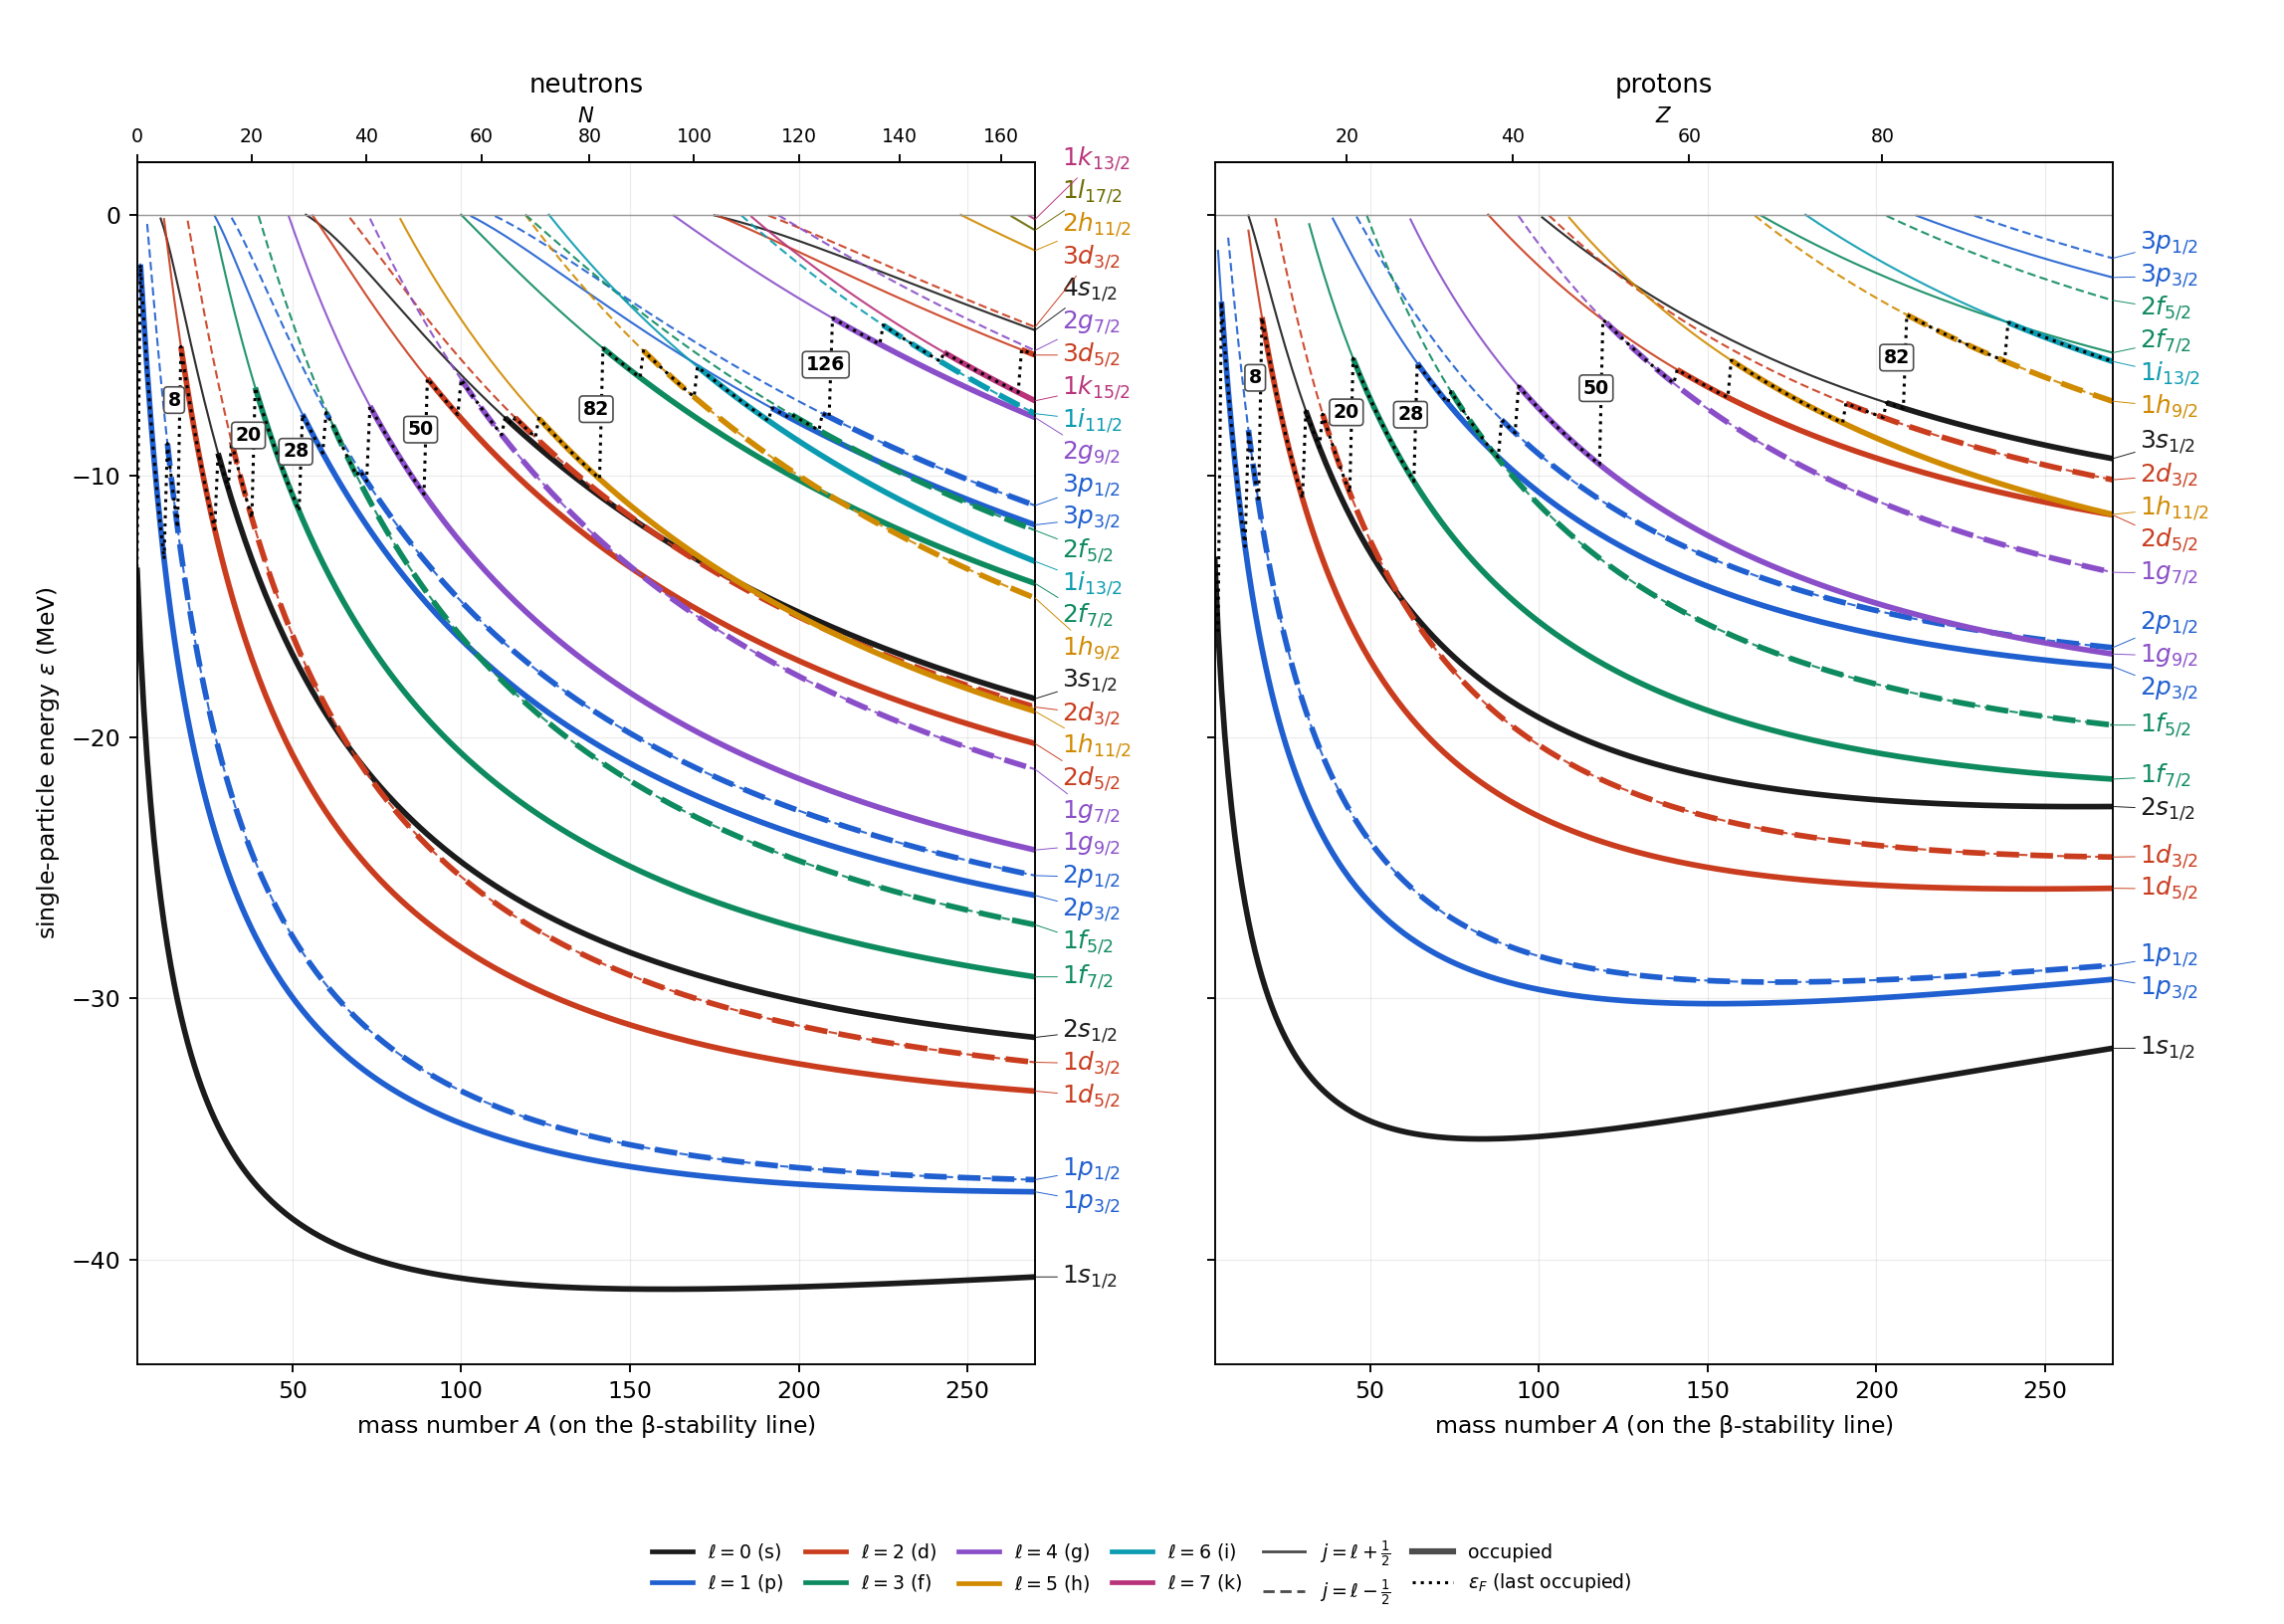
\includegraphics[width=1.0\linewidth]{sp_evolution_A.png}
    \caption{Neutron (left) and proton (right) single-particle levels of the Woods--Saxon potential with spin-orbit and Coulomb terms (Seminole parameters) for nuclei on the $\beta$-stability line, as a function of $A$ (top axis: $N$ or $Z$). Colours label $\ell$; solid lines $j=\ell+\frac12$, dashed $j=\ell-\frac12$. Thick segments are occupied orbits, the dotted line is the last occupied level $\varepsilon_F$, and boxes mark the shell closures. Calculated with the course code \texttt{woods\_saxon\_shells.py}.}
    \label{fig:spevolA}
\end{figure}

\subsection{Spin-orbit interaction}
We add a spin-orbit term
\[
\op U=U(r)-2\alpha\,\op{\vec\ell}\cdot\op{\vec s},\qquad \alpha\ \text{--- strength of the interaction}.
\]
With $\op{\vec j}=\op{\vec\ell}+\op{\vec s}$ (and $\hbar=1$)
\[
\op H_{\rm mf}=\op H^0_{\rm mf}-2\alpha\,\op{\vec\ell}\cdot\op{\vec s}
=\Big(\frac{\op{\vec p}^{\,2}}{2m}+\op U\Big)-\alpha\big(\op{\vec j}^{\,2}-\op{\vec\ell}^{\,2}-\op{\vec s}^{\,2}\big).
\]
If we know the eigenstates of $\op H^0_{\rm mf}$,
\[
\op H^0_{\rm mf}\ket{n\ell m_\ell}=\varepsilon^0_{n\ell}\ket{n\ell m_\ell},\qquad
\braket{\vec r|n\ell m_\ell}=R_{n\ell}(r)\,Y_{\ell m_\ell}(\vartheta,\varphi),
\]
we can easily construct the eigenstates of $\op H_{\rm mf}$:
\[
\ket{n\ell jm}=\sum_{m_\ell,m_s}\big(\ell m_\ell\,\tfrac12 m_s\big|jm\big)\ket{n\ell m_\ell}\ket{s{=}\tfrac12\,m_s},
\]
\[
\op H_{\rm mf}\ket{n\ell jm}=\underbrace{\Big[\varepsilon^0_{n\ell}-\alpha\Big(j(j+1)-\ell(\ell+1)-\tfrac12\big(\tfrac12+1\big)\Big)\Big]}_{\varepsilon_{n\ell j}}\ket{n\ell jm},
\qquad j=\ell-\tfrac12,\ \ell+\tfrac12 .
\]
For $j=\ell+\frac12$:
\[
\varepsilon_{n\ell,j=\ell+1/2}=\varepsilon^0_{n\ell}-\alpha\Big[\big(\ell+\tfrac12\big)\big(\ell+\tfrac32\big)-\ell(\ell+1)-\tfrac34\Big]
=\varepsilon^0_{n\ell}-\alpha\ell=\varepsilon^0_{n\ell}-\alpha\big(j-\tfrac12\big).
\]
For $j=\ell-\frac12$:
\[
\varepsilon_{n\ell,j=\ell-1/2}=\varepsilon^0_{n\ell}-\alpha\Big[\big(\ell-\tfrac12\big)\big(\ell+\tfrac12\big)-\ell(\ell+1)-\tfrac34\Big]
=\varepsilon^0_{n\ell}+\alpha(\ell+1)=\varepsilon^0_{n\ell}+\alpha\big(j+\tfrac32\big).
\]
For the HO with $\alpha>0$ we obtain the following level scheme (energy increasing downwards, each level with degeneracy $2j+1$; the numbers in the last column are the accumulated numbers of particles):
\begin{center}
\begin{tabular}{c l l c r}
$N$ & & & $2j+1$ & total\\ \hline
0 & $1s$ & $1s_{1/2}$ & 2 & \textbf{2} \\ \hline
1 & $1p$ & $1p_{3/2}$ & 4 & \\
  &      & $1p_{1/2}$ & 2 & \textbf{8} \\ \hline
2 & $2s$ & $2s_{1/2}$ & 2 & \\
  & $1d$ & $1d_{5/2}$ & 6 & \textbf{20}\\
  &      & $1d_{3/2}$ & 4 & \\ \hline
3 & $1f$ & $\boxed{1f_{7/2}}$ & 8 & \textbf{28}\\
  &      & $1f_{5/2}$ & 6 & \\
  & $2p$ & $2p_{3/2}$ & 4 & \\
  &      & $2p_{1/2}$ & 2 & 40 \\ \hline
4 & $1g$ & $\boxed{1g_{9/2}}$ & 10 & \textbf{50}\\
  &      & $1g_{7/2}$ & 8 & \\
  & $2d$ & $2d_{5/2}$ & 6 & \\
  &      & $2d_{3/2}$ & 4 & \\
  & $3s$ & $3s_{1/2}$ & 2 & 70\\ \hline
5 & $1h$ & $\boxed{1h_{11/2}}$ & 12 & \textbf{82}\\
  &      & $1h_{9/2}$ & 10 & \\
  & $2f$ & $2f_{7/2}$ & 8 & \\
  &      & $2f_{5/2}$ & 6 & \\
  & $3p$ & $3p_{3/2}$ & 4 & \\
  &      & $3p_{1/2}$ & 2 & 112\\ \hline
6 & $1i$ & $\boxed{1i_{13/2}}$ & 14 & \textbf{126}\\
  &      & $1i_{11/2}$ & 12 & \\
  & $2g$ & $2g_{9/2}$ & 10 & \\
  &      & $2g_{7/2}$ & 8 & \\
  & $3d$ & $3d_{5/2}$ & 6 & \\
  &      & $3d_{3/2}$ & 4 & \\
  & $4s$ & $4s_{1/2}$ & 2 & \\ \hline
\end{tabular}
\end{center}
The levels $1f_{7/2}$, $1g_{9/2}$, $1h_{11/2}$, $1i_{13/2}$ (boxed), due to the spin-orbit splitting, fall down to the lower shells $\Rightarrow$ new shells with the correct magic numbers
\[
2,\ 8,\ 20,\ 28,\ 50,\ 82,\ 126 .
\]
These ``intruder'' states \underline{have opposite parity} than the rest of the shell.

The spin-orbit force is more important at the surface. A ``realistic'' single-particle potential (Woods--Saxon) is
\[
V(r)=\underbrace{-\frac{V_0}{1+e^{(r-R)/a}}}_{U}+\lambda\,\frac{\ud\tilde V}{\ud r}\,\vec\ell\cdot\vec s+V_{\rm Coul},
\qquad
\tilde V=-\frac{\tilde V_0}{1+e^{(r-R)/a}} .
\]
\begin{center}
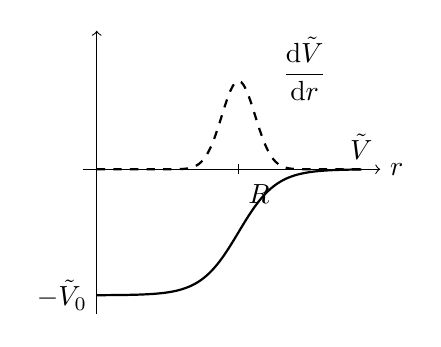
\begin{tikzpicture}[xscale=0.6,yscale=0.8]
\draw[->] (-0.3,0) -- (6,0) node[right]{$r$};
\draw[->] (0,-2.3) -- (0,2.2);
\draw[thick,domain=0:5.6,samples=100,smooth] plot (\x,{-2/(1+exp((\x-3)/0.4))}) node[above]{$\tilde V$};
\draw[thick,dashed,domain=0:5.6,samples=100,smooth] plot (\x,{1.4*exp(-((\x-3)/0.5)^2)});
\node at (4.4,1.6) {$\dfrac{\ud\tilde V}{\ud r}$};
\draw (3,0.08) -- (3,-0.08) node[below right]{$R$};
\node[left] at (0,-2) {$-\tilde V_0$};
\end{tikzpicture}
\end{center}

\paragraph{Note:} The $\vec\ell\cdot\vec s$ interaction exists in atoms too: there it is the interaction of the magnetic moment of the electron with the electromagnetic field (generated by the nucleus). In nuclei, its existence has to be attributed to the $NN$ interaction, but its mechanism is not fully understood. In nuclei the ``parallel'' configuration ($j=\ell+\frac12$) is energetically favourable, in atoms the antiparallel one.

It is good to realize that \underline{single-particle energies are not observables!}
Experimental information about ``single-particle'' states can be guessed from spectra of nuclei with 1 ``valence'' particle (or hole).

\subsection{Single-particle energies from experiment}
If we accept the validity of a mean-field model, we can extract ``experimental'' single-particle energies from the spectra of nuclei neighbouring to magic ones.

\paragraph{Particle states.} Adding a neutron (proton) to the magic core with $A$ nucleons, the separation energy of the nucleus $A+1$ in the state $i$ with excitation energy $E_i^{A+1}$ is
\[
S^{A+1}_{n(p)}=-\varepsilon^i_{n(p)}+E^{A+1}_i ,
\]
\begin{center}
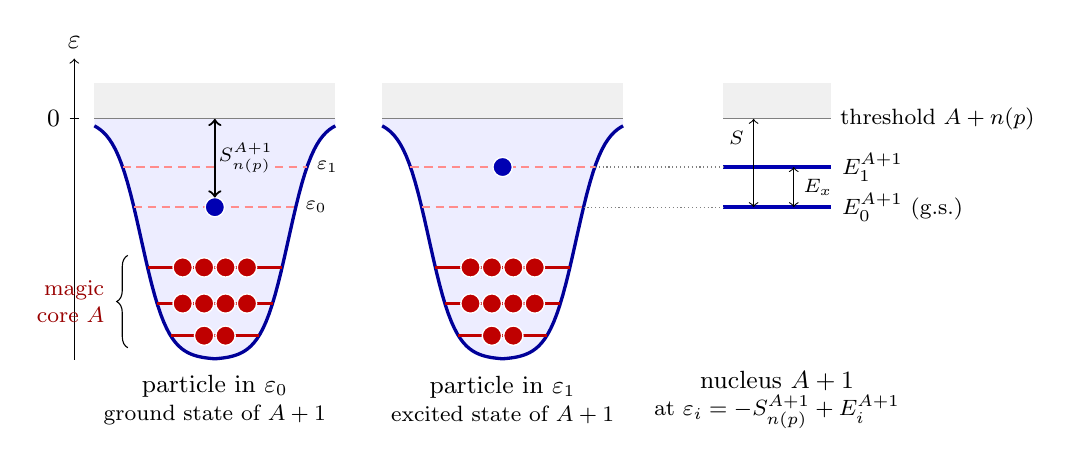
\begin{tikzpicture}[scale=0.85,yscale=1.2]
  \draw[->] (-2.1,-3.0) -- (-2.1,0.75) node[above] {$\varepsilon$};
  \draw (-2.17,0) -- (-2.03,0) node[pos=0,left,font=\small] {$0$};
  % ground state of A+1
  \begin{scope}
    \spwell \spcore \splev{-1.85}{core,core,core,core}
    \splev[emptylev]{-1.1}{val} \spempty{-0.6}
    \node[font=\scriptsize,right] at ({xw(-1.1)},-1.1) {$\varepsilon_0$};
    \node[font=\scriptsize,right] at ({xw(-0.6)},-0.6) {$\varepsilon_1$};
    \draw[decorate,decoration={brace,amplitude=4pt,mirror}] (-1.3,-1.7) -- (-1.3,-2.85)
       node[midway,left=5pt,font=\footnotesize,align=right,red!60!black] {magic\\core $A$};
    \draw[<->,thick] (0,-0.98) -- (0,0) node[midway,right,font=\scriptsize,fill=blue!7,inner sep=1pt] {$S^{A+1}_{n(p)}$};
    \node[font=\small,align=center] at (0,-3.5) {particle in $\varepsilon_0$\\[-1pt] {\footnotesize ground state of $A+1$}};
  \end{scope}
  % excited state of A+1
  \begin{scope}[xshift=4.3cm]
    \spwell \spcore \splev{-1.85}{core,core,core,core}
    \spempty{-1.1} \splev[emptylev]{-0.6}{val}
    \node[font=\small,align=center] at (0,-3.5) {particle in $\varepsilon_1$\\[-1pt] {\footnotesize excited state of $A+1$}};
  \end{scope}
  % states of A+1 on the same energy scale
  \begin{scope}[xshift=7.6cm]
    \fill[gray!12] (0,0) rectangle (1.6,0.45);
    \draw[gray] (0,0) -- (1.6,0) node[right,black,font=\footnotesize] {threshold $A+n(p)$};
    \draw[ultra thick,blue!70!black] (0,-1.1) -- (1.6,-1.1) node[right,black,font=\footnotesize] {$E_0^{A+1}$ (g.s.)};
    \draw[ultra thick,blue!70!black] (0,-0.6) -- (1.6,-0.6) node[right,black,font=\footnotesize] {$E_1^{A+1}$};
    \draw[<->] (0.45,-1.1) -- (0.45,0) node[pos=0.78,left,font=\scriptsize] {$S$};
    \draw[<->] (1.05,-1.1) -- (1.05,-0.6) node[midway,right,font=\scriptsize] {$E_x$};
    \node[font=\small,align=center] at (0.8,-3.5) {nucleus $A+1$\\[-1pt] {\footnotesize at $\varepsilon_i=-S^{A+1}_{n(p)}+E_i^{A+1}$}};
  \end{scope}
  \foreach \e in {-1.1,-0.6} \draw[densely dotted,gray] ({4.3+xw(\e)},\e) -- (7.6,\e);
\end{tikzpicture}
\end{center}
or in terms of binding energies
\[
B^{A+1}_{Z(Z+1)}-B^A_Z-E^{A+1}_i=-\varepsilon^i_{n(p)}
\quad\Longrightarrow\quad
\varepsilon^i_{n(p)}=B^A_Z-B^{A+1}_{Z(Z+1)}+E^{A+1}_i .
\]
E.g.\ from ${}^{17}$O we get information about neutron particle states in ${}^{16}$O, from ${}^{209}$Bi about proton particle states in ${}^{208}$Pb, \dots

\paragraph{Hole states.} Removing a nucleon from the magic nucleus $A$, the nucleus $A-1$ is left in the state $i$:
\[
S^A_{n(p)}=-\varepsilon^i_{n(p)}-E^{A-1}_i ,
\]
\begin{center}
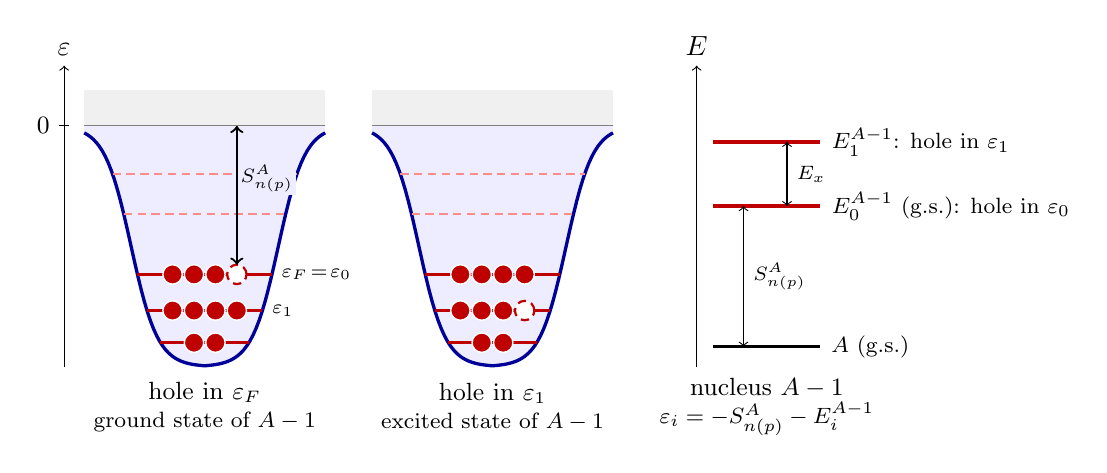
\begin{tikzpicture}[scale=0.85,yscale=1.2]
  \draw[->] (-2.1,-3.0) -- (-2.1,0.75) node[above] {$\varepsilon$};
  \draw (-2.17,0) -- (-2.03,0) node[pos=0,left,font=\small] {$0$};
  \begin{scope}
    \spwell \spcore \splev{-1.85}{core,core,core,hole}
    \spempty{-1.1} \spempty{-0.6}
    \node[font=\scriptsize,right] at ({xw(-1.85)},-1.85) {$\varepsilon_F\!=\!\varepsilon_0$};
    \node[font=\scriptsize,right] at ({xw(-2.3)},-2.3) {$\varepsilon_1$};
    \draw[<->,thick] (0.48,-1.73) -- (0.48,0) node[pos=0.62,right,font=\scriptsize,fill=blue!7,inner sep=1pt] {$S^{A}_{n(p)}$};
    \node[font=\small,align=center] at (0,-3.5) {hole in $\varepsilon_F$\\[-1pt] {\footnotesize ground state of $A-1$}};
  \end{scope}
  \begin{scope}[xshift=4.3cm]
    \spwell \splev{-2.7}{core,core}\splev{-2.3}{core,core,core,hole}\splev{-1.85}{core,core,core,core}
    \spempty{-1.1} \spempty{-0.6}
    \node[font=\small,align=center] at (0,-3.5) {hole in $\varepsilon_1$\\[-1pt] {\footnotesize excited state of $A-1$}};
  \end{scope}
  \begin{scope}[xshift=7.6cm]
    \draw[->] (-0.25,-3.0) -- (-0.25,0.75) node[above] {$E$};
    \draw[very thick] (0,-2.75) -- (1.6,-2.75) node[right,font=\footnotesize] {$A$ (g.s.)};
    \draw[ultra thick,red!75!black] (0,-1.0) -- (1.6,-1.0) node[right,black,font=\footnotesize] {$E_0^{A-1}$ (g.s.): hole in $\varepsilon_0$};
    \draw[ultra thick,red!75!black] (0,-0.2) -- (1.6,-0.2) node[right,black,font=\footnotesize] {$E_1^{A-1}$: hole in $\varepsilon_1$};
    \draw[<->] (0.45,-2.75) -- (0.45,-1.0) node[midway,right,font=\scriptsize] {$S^{A}_{n(p)}$};
    \draw[<->] (1.1,-1.0) -- (1.1,-0.2) node[midway,right,font=\scriptsize] {$E_x$};
    \node[font=\small,align=center] at (0.8,-3.5) {nucleus $A-1$\\[-1pt] {\footnotesize $\varepsilon_i=-S^{A}_{n(p)}-E_i^{A-1}$}};
  \end{scope}
\end{tikzpicture}
\end{center}
\[
B^A_Z-B^{A-1}_{Z(Z-1)}+E^{A-1}_i=-\varepsilon^i_{n(p)}
\quad\Longrightarrow\quad
\varepsilon^i_{n(p)}=B^{A-1}_{Z(Z-1)}-B^A_Z-E^{A-1}_i .
\]
E.g.\ from the spectrum of ${}^{207}$Pb we get information about the hole states of ${}^{208}$Pb, \dots

\subsection{Limits and use of the single-particle picture}
In spite of the formal similarity with the QM model of the atom, the mechanism responsible for the appearance of shells in nuclei is different. In nuclei, no external field (like the Coulomb field of the atomic nucleus) exists. The nuclear mean field is a result of ``averaging'' of complicated 2-, 3-, \dots body interactions among the nucleons.

Pure ``single-particle'' states do not exist in nuclei. ``Experimental single-particle levels'' must be understood as a result of the expansion of the many-body wave function into the ``shell-model basis'', represented by e.g.\ Slater determinants:
\[
\Psi=c_0\,\big|\text{magic core}+1\ \text{``valence'' nucleon}\big\rangle
+c_1\,\big|2\text{p--}1\text{h}\big\rangle
+c_2\,\big|3\text{p--}2\text{h}\big\rangle+\dots
\]
\begin{center}
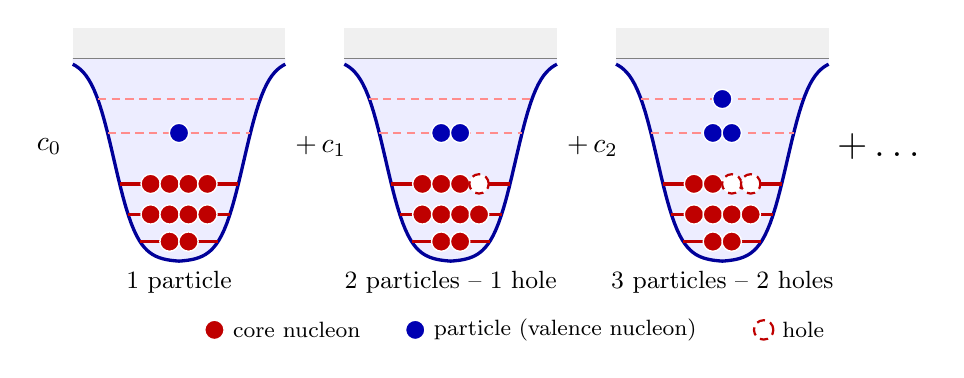
\begin{tikzpicture}[scale=0.75,yscale=1.15]
  \foreach \xs/\c/\lab in {0/{c_0}/{1 particle}, 4.6/{+\,c_1}/{2 particles -- 1 hole}, 9.2/{+\,c_2}/{3 particles -- 2 holes}} {
    \begin{scope}[xshift=\xs cm]
      \spwell \spcore
      \node[font=\normalsize] at (-2.2,-1.3) {$\c$};
      \node[font=\small] at (0,-3.3) {\lab};
    \end{scope}}
  \begin{scope}
    \splev{-1.85}{core,core,core,core} \splev[emptylev]{-1.1}{val} \spempty{-0.6}
  \end{scope}
  \begin{scope}[xshift=4.6cm]
    \splev{-1.85}{core,core,core,hole} \splev[emptylev]{-1.1}{val,val} \spempty{-0.6}
  \end{scope}
  \begin{scope}[xshift=9.2cm]
    \splev{-1.85}{core,core,hole,hole} \splev[emptylev]{-1.1}{val,val} \splev[emptylev]{-0.6}{val}
  \end{scope}
  \node[font=\Large] at (11.9,-1.3) {$+\dots$};
  \begin{scope}[shift={(0.6,-4.0)},font=\footnotesize]
    \node[core] at (0,0) {}; \node[right] at (0.15,0) {core nucleon};
    \node[val] at (3.4,0) {}; \node[right] at (3.55,0) {particle (valence nucleon)};
    \node[hole] at (9.3,0) {}; \node[right] at (9.45,0) {hole};
  \end{scope}
\end{tikzpicture}
\end{center}
One may hope that for some states $c_0^2\gg c_1^2,c_2^2,\dots$, i.e.\ $|c_0|^2\approx1$ $\Rightarrow$ single-particle state. In reality $|c_0|^2<1$. Therefore the 1p (one particle) or 1h (one hole) states are just approximations! But they are useful for some predictions.

\paragraph{Spin and parity.} A valence nucleon in the orbit $\ket{n\ell jm}$ above an inert (even-even) core with $I^\pi=0^+$ determines the spin and parity of the nucleus:
\[
\vec J=\vec I+\vec j=\vec j\ \Rightarrow\ J=j,\qquad \pi=(-1)^\ell .
\]
A similar picture can be used for ``hole'' configurations: the hole in the orbit $j$ together with the remaining nucleons with spin $J$ couple to the spin of the closed core, $\vec j+\vec J=\vec I=0$, hence
\[
J=j,\qquad \pi=(-1)^\ell .
\]
If more nucleons occupy a $j$-shell, pairs with total angular momentum 0 can be formed. E.g.\ for 3 nucleons in the $d_{5/2}$ shell
\[
I\big[(d_{5/2})^3\big]=I\big[d_{5/2}\big]=\tfrac52 .
\]

\subsection{Magnetic dipole moments in the single-particle model}
One can calculate magnetic dipole moments in the single-particle model for nuclei with 1 valence nucleon (or 1 hole). The contribution from the core vanishes, $\mu_c=0$ $\Rightarrow$ the magnetic moment is given by the single-particle orbit $\ket{n\ell jm}$:
\[
\mu=\braket{n\ell j\,m{=}j|\op\mu_z|n\ell j\,m{=}j},
\qquad
\op\mu_z=\mu_N\big(g_\ell\op\ell_z+g_s\op s_z\big)=\mu_N\big[g_\ell\op j_z+(g_s-g_\ell)\op s_z\big],
\qquad \op j_z=\op\ell_z+\op s_z ,
\]
with the single-particle wave function
\[
\braket{\vec r\sigma|n\ell jm}=\phi_{n\ell jm}=R_{n\ell}(r)\sum_{m_\ell,m_s}\big(\ell m_\ell\,\tfrac12 m_s\big|jm\big)\,Y_{\ell m_\ell}(\vartheta,\varphi)\,\chi^{1/2}_{m_s}.
\]
Then
\[
\mu=\mu_N\braket{n\ell jj|g_\ell\op j_z+(g_s-g_\ell)\op s_z|n\ell jj}
\]
\[
=\mu_N\int_0^\infty|R_{n\ell}|^2r^2\ud r\,\Big\{g_\ell\,j+(g_s-g_\ell)\sum_{m_\ell,m_s}\big(\ell m_\ell\,\tfrac12 m_s\big|jj\big)^2m_s\Big\},
\]
because
\[
\int\ud\Omega\,Y^*_{\ell m_\ell}Y_{\ell' m'_\ell}=\delta_{\ell\ell'}\delta_{m_\ell m'_\ell},
\qquad
\chi^{1/2\,\dagger}_{m_s}\,\op s_z\,\chi^{1/2}_{m'_s}=\delta_{m_sm'_s}\,m'_s .
\]
For $j=\ell+\frac12$, with $\big(\ell\ell\,\tfrac12\tfrac12\big|\ell{+}\tfrac12\,\ell{+}\tfrac12\big)=1$:
\[
\mu_{\ell+1/2}=\mu_N\Big[g_\ell j+(g_s-g_\ell)\cdot1\cdot\tfrac12\Big]
=\mu_N\,j\Big(\underbrace{g_\ell+\frac{g_s-g_\ell}{2\ell+1}}_{g}\Big).
\]
For $j=\ell-\frac12$, with
\[
\big(\ell\,\ell{-}1\,\tfrac12\tfrac12\big|\ell{-}\tfrac12\,\ell{-}\tfrac12\big)=-\frac{1}{\sqrt{2\ell+1}},
\qquad
\big(\ell\,\ell\,\tfrac12\,{-}\tfrac12\big|\ell{-}\tfrac12\,\ell{-}\tfrac12\big)=\sqrt{\frac{2\ell}{2\ell+1}},
\]
\[
\mu_{\ell-1/2}=\mu_N\Big[g_\ell j+(g_s-g_\ell)\Big\{\big(\ell\,\ell{-}1\,\tfrac12\tfrac12\big|\ell{-}\tfrac12\,\ell{-}\tfrac12\big)^2\tfrac12
-\big(\ell\,\ell\,\tfrac12\,{-}\tfrac12\big|\ell{-}\tfrac12\,\ell{-}\tfrac12\big)^2\tfrac12\Big\}\Big]
\]
\[
=\mu_N\Big[g_\ell j+(g_s-g_\ell)\frac{1}{2\ell+1}\,\frac12(1-2\ell)\Big]
=\mu_N\,j\Big[g_\ell-(g_s-g_\ell)\frac{1}{2\ell+1}\Big].
\]
Together
\[
\mu_{\ell\pm1/2}=\mu_N\,j\underbrace{\Big[g_\ell\pm(g_s-g_\ell)\frac{1}{2\ell+1}\Big]}_{g\ \text{--- gyromagnetic factor}} .
\]
For protons, $g_s^p=5.59$, $g_\ell^p=1$:
\[
\mu_{\ell+1/2}=\mu_N\big[j+2.29\big],\qquad
\mu_{\ell-1/2}=\mu_N\,j\Big[1-\frac{2.29}{j+1}\Big].
\]
For neutrons, $g_s^n=-3.83$, $g_\ell^n=0$:
\[
\mu_{\ell+1/2}=\mu_N\big[-1.91\big],\qquad
\mu_{\ell-1/2}=\mu_N\Big[1.91\,\frac{j}{j+1}\Big].
\]
These are the \textbf{Schmidt estimates} for $\mu$.

Examples:
\begin{itemize}
\item ${}^{17}_{\ 9}$F: proton particle in $1d_{5/2}$ $\to$ $\frac52^+$, $j=\ell+\frac12$;
\item ${}^{209}$Bi: proton particle in $1h_{9/2}$ $\to$ $\frac92^-$, $j=\ell-\frac12$;
\item ${}^{207}$Pb: neutron hole in $3p_{1/2}$ $\to$ $\frac12^-$, $j=\ell-\frac12$.
\end{itemize}
The magnetic moment for a hole configuration is given by the corresponding single-particle state.

Fig.~\ref{fig:schmidt} compares the Schmidt lines with the measured ground-state magnetic moments of nuclei that have one nucleon more (particle) or one nucleon less (hole) than a doubly magic core (${}^{16}$O, ${}^{40}$Ca, ${}^{48}$Ca, ${}^{56}$Ni, ${}^{132}$Sn, ${}^{208}$Pb). The orbit $n\ell j$ follows from the measured $I^\pi$; e.g.\ ${}^{39}$K ($\frac32^+$) is a proton hole in $1d_{3/2}$ ($\ell=2$, $j=\ell-\frac12$), and ${}^{57}$Cu ($\frac32^-$) is a proton in $2p_{3/2}$ ($\ell=1$, $j=\ell+\frac12$). We can see that:
\begin{itemize}
\item the light nuclei ${}^{15}$N, ${}^{17}$F, ${}^{15}$O, ${}^{17}$O, ${}^{39}$Ca and the heavy ${}^{207}$Pb are within $\approx0.1$--$0.15\,\mu_N$ of the Schmidt values, i.e.\ they are good single-particle (single-hole) states;
\item larger deviations appear e.g.\ for ${}^{209}$Bi ($4.11\,\mu_N$ vs.\ $2.62\,\mu_N$), ${}^{207}$Tl ($1.88$ vs.\ $2.79$), ${}^{57}$Cu ($2.58$ vs.\ $3.79$) or ${}^{57}$Ni ($-0.80$ vs.\ $-1.91$);
\item the measured values are (almost) always shifted from the Schmidt line towards the other line, i.e.\ the spin contribution is reduced; the dashed lines show the result with $g_s^{\rm eff}=0.7\,g_s$ (see below).
\end{itemize}
\begin{figure}[htbp]
    \centering
    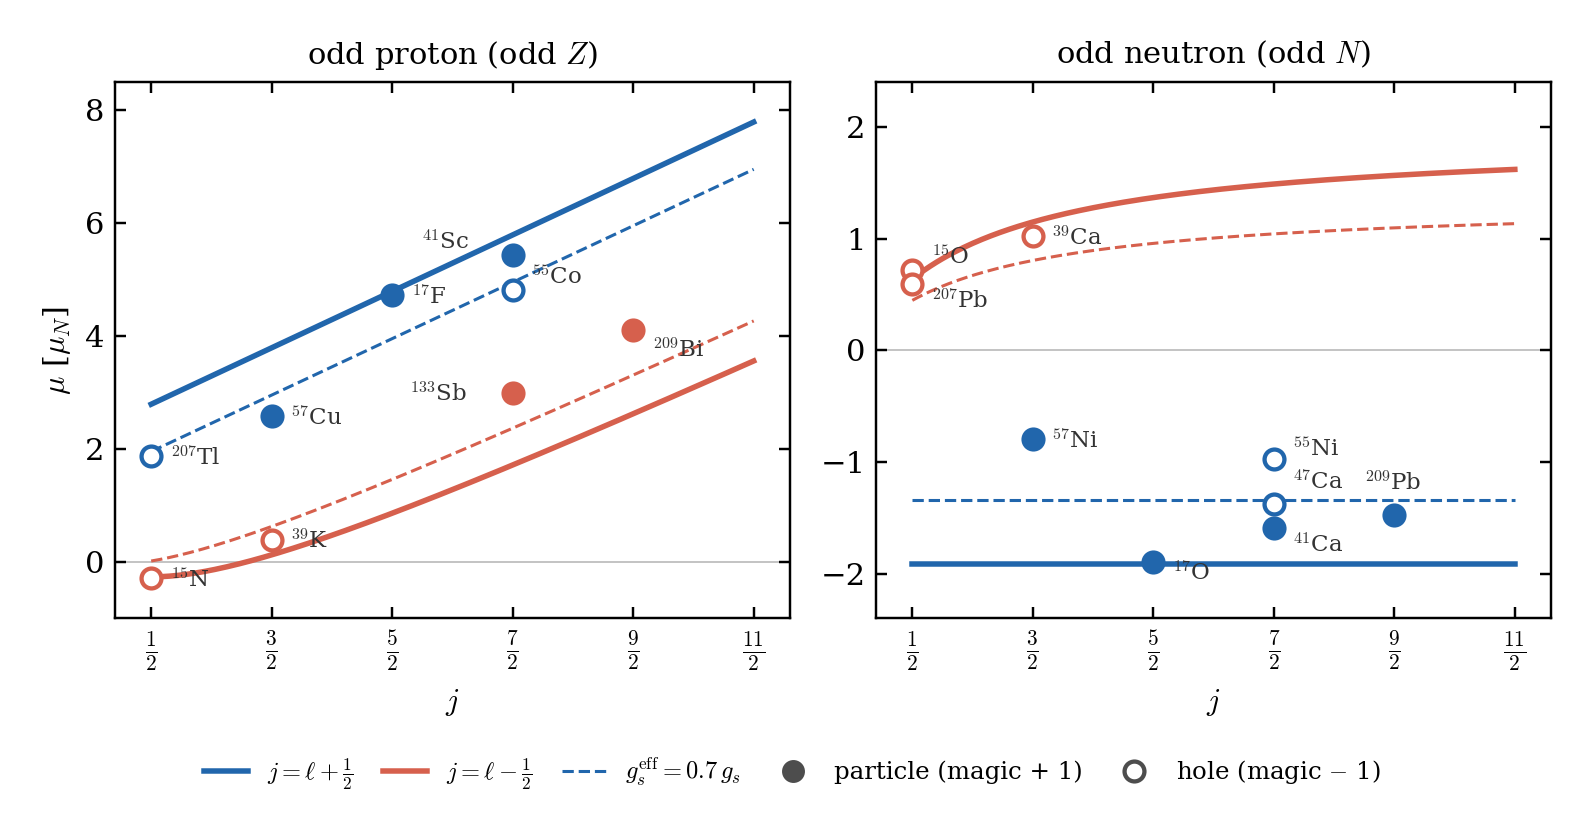
\includegraphics[width=\linewidth]{schmidt_lines.png}
    \caption{Schmidt lines $\mu(j)=j\big[g_\ell\pm(g_s-g_\ell)/(2\ell+1)\big]$ for $j=\ell+\frac12$ (blue) and $j=\ell-\frac12$ (red), for odd-proton (left) and odd-neutron (right) nuclei. The dashed lines use a quenched spin $g$-factor $g_s^{\rm eff}=0.7\,g_s$. Symbols: measured ground-state magnetic moments of doubly magic $\pm1$ nucleon nuclei; full symbols = particle (magic $+1$), open symbols = hole (magic $-1$), the colour indicating $j=\ell\pm\frac12$ of the occupied orbit. Data: N.~J.~Stone, At.\ Data Nucl.\ Data Tables \textbf{90} (2005) 75; IAEA report INDC(NDS)-0658 (2014).}
    \label{fig:schmidt}
\end{figure}

The observed magnetic moments lie within the bands given by the Schmidt estimates, or at least not far from them; nuclei magic $\pm1$ nucleon are closer to the Schmidt estimates. The agreement improves using an effective spin $g$-factor
\[
g_s\ \to\ g_s^{\rm eff}=x\cdot g_s,\qquad x<1\ \to\ \text{core polarization effect},
\]
\[
\mu=j\Big(g_\ell\pm\big(g_s^{\rm eff}-g_\ell\big)\frac{1}{2\ell+1}\Big),
\]
which mimics admixtures of more complicated configurations (1p $+$ 2p1h $+\dots$).

Part of the $NN$ interaction tends to orient the spins of nucleons of the same type ($pp$, $nn$) antiparallel and of different kind ($pn$) parallel. Since $g_s^p>0$ and $g_s^n<0$, the contribution of the core to $\mu$ is opposite to that from the valence nucleon:
\begin{center}
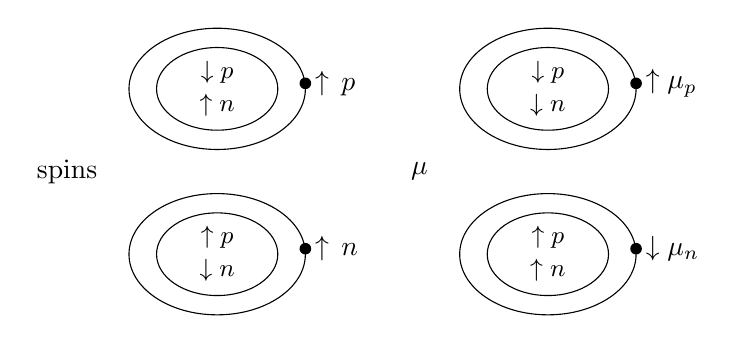
\begin{tikzpicture}[scale=0.7]
\foreach \yy/\val/\cs/\cpm/\cnm in {0/p/$\downarrow$/$\downarrow$/$\uparrow$, -3/n/$\downarrow$/$\uparrow$/$\downarrow$} {
\draw (0,\yy) ellipse (1.6 and 1.1); \draw (0,\yy) ellipse (1.1 and 0.75);
\fill (1.6,\yy+0.1) circle (3pt) node[right]{$\uparrow\,\val$};
}
\node at (0,0.3) {\small $\downarrow p$}; \node at (0,-0.3) {\small $\uparrow n$};
\node at (0,-2.7) {\small $\uparrow p$}; \node at (0,-3.3) {\small $\downarrow n$};
\node[left] at (-2,-1.5) {spins};
\begin{scope}[xshift=6cm]
\draw (0,0) ellipse (1.6 and 1.1); \draw (0,0) ellipse (1.1 and 0.75);
\fill (1.6,0.1) circle (3pt) node[right]{$\uparrow\mu_p$};
\node at (0,0.3) {\small $\downarrow p$}; \node at (0,-0.3) {\small $\downarrow n$};
\draw (0,-3) ellipse (1.6 and 1.1); \draw (0,-3) ellipse (1.1 and 0.75);
\fill (1.6,-2.9) circle (3pt) node[right]{$\downarrow\mu_n$};
\node at (0,-2.7) {\small $\uparrow p$}; \node at (0,-3.3) {\small $\uparrow n$};
\node[left] at (-2,-1.5) {$\mu$};
\end{scope}
\end{tikzpicture}
\end{center}
Hence $|g_s^{\rm eff}|<|g_s|$ for most nuclei.

\subsection{Electric quadrupole moments in the single-particle model}
One can easily calculate the electric quadrupole moment generated by a valence nucleon,
\[
\op Q_{33}=3\op z_p^2-\op r_p^2=\op r_p^2\Big(\frac{16\pi}{5}\Big)^{1/2}Y_{20}(\vartheta,\varphi),
\]
$\Rightarrow$ only a proton contributes $\Rightarrow$ single-particle $Q$. One obtains
\[
Q_{\rm s.p.}=\braket{n\ell jj|\op Q_{33}|n\ell jj}=-\frac{2j-1}{2j+2}\,\braket{r^2}_{n\ell}.
\]
Moreover
\[
Q_{\rm s.p.}(\text{hole})=-Q_{\rm s.p.}(\text{particle}),
\]
i.e.\ the hole might be understood to have an opposite charge.

For odd-$N$ nuclei, the extreme single-particle model predicts $Q_{\rm s.p.}=0$, but experimental values are comparable to those of odd-$Z$ nuclei. This can be understood as a ``polarization'' of the core by the valence nucleon --- an analogy with tidal waves:
\begin{center}
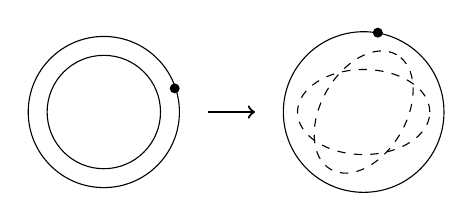
\begin{tikzpicture}[scale=0.6]
\draw (0,0) circle (1.6); \draw (0,0) circle (1.2);
\fill (1.5,0.5) circle (3pt);
\draw[->,thick] (2.2,0) -- (3.2,0);
\begin{scope}[xshift=5.5cm]
\draw (0,0) circle (1.7);
\draw[dashed] (0,0) ellipse (1.4 and 0.9);
\draw[dashed,rotate=60] (0,0) ellipse (1.4 and 0.9);
\fill (0.3,1.68) circle (3pt);
\end{scope}
\end{tikzpicture}
\end{center}
For many nuclei $|Q|$ is much larger than $Q_{\rm s.p.}$ $\Rightarrow$ \textbf{deformation of the mean field}.

%=====================================================================
\subsection{A short note about the Hartree--Fock method}
%=====================================================================
The mean field can be in principle calculated from the $NN$ interaction. For a set of single-particle states $\varphi_\alpha(\vec r)$ (energies $\varepsilon_\alpha$, occupied up to the Fermi level $\varepsilon_F$), the ground-state density is given by
\[
\rho(\vec r)=\sum_{i\le\varepsilon_F}\varphi_i^*(\vec r)\,\varphi_i(\vec r).
\]
Nucleons interact via a 2-body interaction $V(\vec r,\vec r\,')$ (also other degrees of freedom like spin and isospin can be considered). The mean potential at position $\vec r$ is certainly given by summing of all contributions, i.e.
\[
U_H(\vec r)=\int V(\vec r,\vec r\,')\,\rho(\vec r\,')\,\ud^3r'
=\sum_{i\le\varepsilon_F}\int\varphi_i^*(\vec r\,')\,V(\vec r,\vec r\,')\,\varphi_i(\vec r\,')\,\ud^3r' .
\]
The Schr\"odinger equation for a single-particle state is then
\[
\Big[-\frac{\hbar^2}{2m}\Delta+U_H(\vec r)\Big]\varphi_b(\vec r)=\varepsilon_b\,\varphi_b(\vec r),\qquad b=1,2,\dots
\]
This set of integro-differential equations represents a \textbf{self-consistent} problem, because the so-called Hartree potential $U_H$ depends on the solutions $\varphi_i$. One can find such states $\varphi_i$ which generate an average potential $U_H$ whose single-particle eigenfunctions are the same $\varphi_i$ wave functions.

In order to take into account antisymmetrization (Pauli principle), one can show that the Fock (exchange) term must be included into the Schr\"odinger equation, $\varphi_i(\vec r\,')\varphi_b(\vec r)\to\varphi_i(\vec r\,')\varphi_b(\vec r)-\varphi_i(\vec r)\varphi_b(\vec r\,')$:
\[
\underbrace{\sum_{i\le\varepsilon_F}\int\varphi_i^*(\vec r\,')V(\vec r,\vec r\,')\varphi_i(\vec r\,')\,\ud^3r'}_{U_H(\vec r)}\;\varphi_b(\vec r)
\ \longrightarrow\
\sum_{i\le\varepsilon_F}\int\varphi_i^*(\vec r\,')V(\vec r,\vec r\,')\big[\varphi_i(\vec r\,')\varphi_b(\vec r)-\varphi_i(\vec r)\varphi_b(\vec r\,')\big]\ud^3r' .
\]
This leads to the \textbf{Hartree--Fock equations}
\[
\Big[-\frac{\hbar^2}{2m}\Delta+U_H(\vec r)\Big]\varphi_b(\vec r)-\int U_F(\vec r,\vec r\,')\,\varphi_b(\vec r\,')\,\ud^3r'=\varepsilon_b\,\varphi_b(\vec r),
\]
where
\[
U_H(\vec r)=\sum_{i\le\varepsilon_F}\int\varphi_i^*(\vec r\,')\,V(\vec r,\vec r\,')\,\varphi_i(\vec r\,')\,\ud^3r'
\quad\text{is the local Hartree potential},
\]
\[
U_F(\vec r,\vec r\,')=\sum_{i\le\varepsilon_F}\varphi_i^*(\vec r\,')\,V(\vec r,\vec r\,')\,\varphi_i(\vec r)
\quad\text{is the non-local Fock potential}.
\]
The HF equations can be solved iteratively,
\[
\varphi_i^{(0)}(\vec r)\ \to\ U_F^{(0)},U_H^{(0)}\ \to\ \varphi_i^{(1)},\varepsilon_i^{(1)}\ \to\ U_F^{(1)},U_H^{(1)}\ \to\ \varphi_i^{(2)},\varepsilon_i^{(2)}\ \to\ \dots
\]
until convergence is achieved, $|\varepsilon_i^{(k)}-\varepsilon_i^{(k-1)}|\le\varepsilon$ $\forall i$.

One can show that the HF solution provides the variational minimum for the energy
\[
E_{\rm HF}\equiv\braket{\Psi|\op H|\Psi}
\]
if we restrict $\ket\Psi$ to Slater determinants
\[
\Psi=\frac{1}{\sqrt{A!}}
\begin{vmatrix}
\varphi_1(\vec r_1)&\varphi_1(\vec r_2)&\cdots\\
\varphi_2(\vec r_1)&\varphi_2(\vec r_2)&\cdots\\
\vdots&&\ddots
\end{vmatrix}.
\]
In practice, an expansion into a set of known, physically suitable single-particle basis (e.g.\ HO) is used for the determination of HF solutions,
\[
\varphi_i(\vec r)=\sum_k a^i_k\,\varphi^{\rm HO}_k(\vec r),
\]
where $\varphi^{\rm HO}_k$ are the single-particle states of the 3D HO. This allows us to convert the problem to a diagonalisation. The HF basis represents a basis which is often used in ``beyond mean-field'' calculations.

%=====================================================================
\section{Two-particle states --- identical nucleons}
%=====================================================================
Shell-model description of 2 (identical) particles $+$ core:
\[
\op H=\underbrace{\op H_C}_{\text{core}}+\underbrace{\op H_V}_{\text{valence particles}}+\cancel{\op V_{CV}},
\qquad
\op H_V=\underbrace{\op h_0(1)+\op h_0(2)}_{\text{one-body}}+\underbrace{\op V(1,2)}_{\text{two-body}},
\]
where we neglect the interaction $\op V_{CV}$ between the core and the valence space.
The single-particle orbits are divided into three groups: the orbits of the \emph{inert core} are fully occupied and never excited, the \emph{valence space} contains the orbits available to the valence particles, and the orbits above it are always empty (excluded space), see Fig.~\ref{fig:valspace}.
\begin{figure}[htbp]
\centering
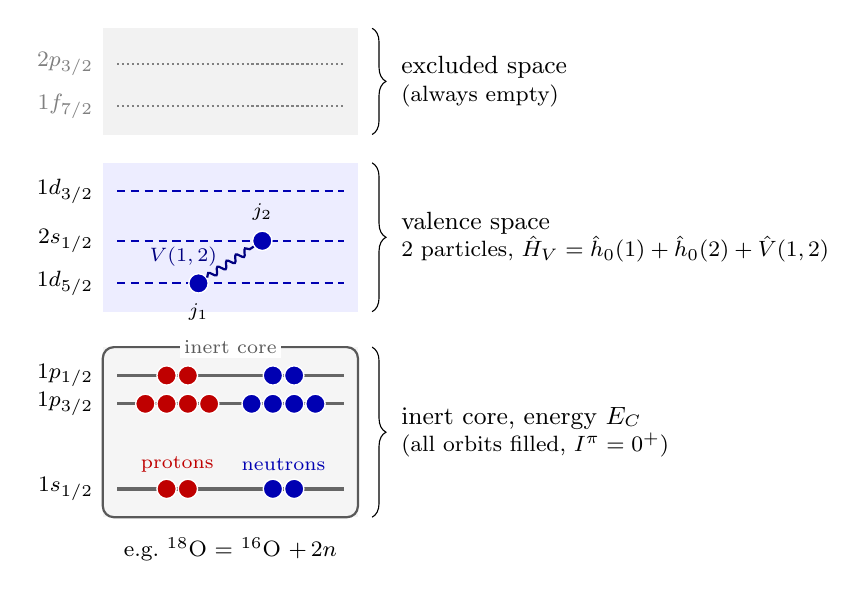
\begin{tikzpicture}[scale=0.9]
  % bands
  \fill[black!4]  (-0.2,-4.0) rectangle (3.4,-1.6);
  \draw[black!65,thick,rounded corners=4pt] (-0.2,-4.0) rectangle (3.4,-1.6);
  \node[font=\scriptsize,black!65,fill=white,inner sep=1.5pt] at (1.6,-1.6) {inert core};
  \fill[blue!7] (-0.2,-1.1) rectangle (3.4,1.0);
  \fill[gray!10] (-0.2,1.4) rectangle (3.4,2.9);
  % core orbits (fully occupied)
  \foreach \y/\lab/\d in {-3.6/1s_{1/2}/2, -2.4/1p_{3/2}/4, -2.0/1p_{1/2}/2} {
    \draw[very thick,black!60] (0,\y) -- (3.2,\y);
    \node[left,font=\footnotesize] at (-0.2,\y) {$\lab$};
    \foreach \k in {1,...,\d} {
      \node[core] at ({0.85+0.3*(\k-(\d+1)/2)},\y) {};
      \node[val]  at ({2.35+0.3*(\k-(\d+1)/2)},\y) {};
    }
  }
  \node[font=\scriptsize,red!75!black] at (0.85,-3.25) {protons};
  \node[font=\scriptsize,blue!70!black] at (2.35,-3.25) {neutrons};
  % valence orbits
  \foreach \y/\lab in {-0.7/1d_{5/2}, -0.1/2s_{1/2}, 0.6/1d_{3/2}} {
    \draw[thick,blue!70!black,densely dashed] (0,\y) -- (3.2,\y);
    \node[left,font=\footnotesize] at (-0.2,\y) {$\lab$};
  }
  \node[val] (p1) at (1.15,-0.7) {};
  \node[val] (p2) at (2.05,-0.1) {};
  \draw[decorate,decoration={snake,amplitude=1.2pt,segment length=4pt},thick,blue!50!black] (p1) -- (p2);
  \node[font=\scriptsize,blue!50!black,left] at (1.55,-0.33) {$V(1,2)$};
  \node[font=\scriptsize,below] at (p1.south) {$j_1$};
  \node[font=\scriptsize,above] at (p2.north) {$j_2$};
  % excluded orbits
  \foreach \y/\lab in {1.8/1f_{7/2}, 2.4/2p_{3/2}} {
    \draw[gray,densely dotted,thick] (0,\y) -- (3.2,\y);
    \node[left,font=\footnotesize,gray] at (-0.2,\y) {$\lab$};
  }
  % braces
  \draw[decorate,decoration={brace,amplitude=5pt}] (3.6,2.9) -- (3.6,1.4)
     node[midway,right=7pt,align=left,font=\small] {excluded space\\[-1pt]{\footnotesize (always empty)}};
  \draw[decorate,decoration={brace,amplitude=5pt}] (3.6,1.0) -- (3.6,-1.1)
     node[midway,right=7pt,align=left,font=\small] {valence space\\[-1pt]{\footnotesize 2 particles, $\op H_V=\op h_0(1)+\op h_0(2)+\op V(1,2)$}};
  \draw[decorate,decoration={brace,amplitude=5pt}] (3.6,-1.6) -- (3.6,-4.0)
     node[midway,right=7pt,align=left,font=\small] {inert core, energy $E_C$\\[-1pt]{\footnotesize (all orbits filled, $I^\pi=0^+$)}};
  \node[font=\footnotesize,align=center] at (1.6,-4.45) {e.g.\ ${}^{18}$O $=$ ${}^{16}$O $+\,2n$};
\end{tikzpicture}
\caption{Shell model with two valence particles. The core orbits are fully occupied (inert core with energy $E_C$; red: protons, blue: neutrons), the two valence particles (here neutrons) occupy orbits $j_1$, $j_2$ of the valence space and interact via the residual interaction $V(1,2)$; the orbits above the valence space are excluded.}
\label{fig:valspace}
\end{figure}
Without interaction we have the unperturbed energy
\[
\op h\ket{n\ell jm}=\varepsilon\ket{n\ell jm},\qquad \op h=\frac{\op{\vec p}^{\,2}}{2m}+\op U,
\qquad
E_0=E_C+\varepsilon_1+\varepsilon_2 ,
\]
where $E_C$ is the reference energy of the core and $\varepsilon_1,\varepsilon_2$ are the single-particle energies of the states $1\equiv\ket{(n_1\ell_1)j_1m_1}$ and $2\equiv\ket{(n_2\ell_2)j_2m_2}$.

The interaction causes a splitting of the unperturbed level $E_C+\varepsilon_1+\varepsilon_2$ of the states $\ket{j_1j_2;JM}$ due to the residual interaction $V(1,2)$, $|j_1-j_2|\le J\le j_1+j_2$:
\begin{center}
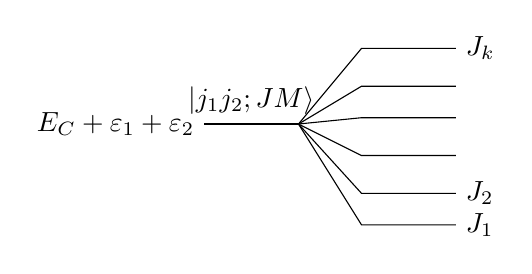
\begin{tikzpicture}[scale=0.8]
\draw (0,0) -- (1.5,0) node[pos=0,left]{$E_C+\varepsilon_1+\varepsilon_2$};
\node[above] at (0.75,0) {$\ket{j_1j_2;JM}$};
\foreach \y/\l in {1.2/J_k, 0.6/, 0.1/, -0.5/, -1.1/J_2, -1.6/J_1} {
\draw (1.5,0) -- (2.5,\y) -- (4,\y) node[right]{$\l$};}
\end{tikzpicture}
\end{center}
$V(1,2)$ is an ``effective'' interaction between valence particles, NOT the bare $NN$ interaction.

The perturbation correction to the energy is given by the diagonal element
\[
E=E_0+\Delta E,\qquad \Delta E(j_1j_2J)=\braket{j_1j_2;JM|\op V(1,2)|j_1j_2;JM}.
\]
In the following we do not consider $E_C$, since it can be understood as a reference energy (we are interested in the energy with respect to the core energy $E_C$).

\subsection{Antisymmetrized two-particle wave function}
With $\braket{\vec r|jm}\equiv\varphi_{jm}(\vec r)$, the antisymmetrized wave function is
\[
\Psi_{\rm as}(j_1j_2,JM)=N\sum_{m_1,m_2}\big(j_1m_1\,j_2m_2\big|JM\big)\Big[\varphi_{j_1m_1}(1)\varphi_{j_2m_2}(2)-\varphi_{j_1m_1}(2)\varphi_{j_2m_2}(1)\Big].
\]
For $j_1\neq j_2$
\[
\Psi_{\rm as}(j_1j_2,JM)=\frac{1}{\sqrt2}\Big[\Psi(j_1j_2,JM)-(-1)^{j_1+j_2-J}\,\Psi(j_2j_1,JM)\Big],
\]
where
\[
\Psi(j_1j_2,JM)=\sum_{m_1,m_2}\big(j_1m_1\,j_2m_2\big|JM\big)\varphi_{j_1m_1}(1)\varphi_{j_2m_2}(2),
\]
\[
\Psi(j_2j_1,JM)=\sum_{m_1,m_2}\underbrace{\big(j_2m_2\,j_1m_1\big|JM\big)}_{(-1)^{j_1+j_2-J}(j_1m_1\,j_2m_2|JM)}\varphi_{j_2m_2}(1)\varphi_{j_1m_1}(2).
\]
For $j_1=j_2\equiv j$
\[
\Psi_{\rm as}(j^2;JM)=N\Big[\Psi(j^2,JM)-(-1)^{2j-J}\,\Psi(j^2,JM)\Big],
\]
which (for half-integer $j=\frac12,\frac32,\dots$) is nonzero only for $J=0,2,4,\dots$, in which case
\[
\Psi_{\rm as}(j^2;JM)=2N\,\Psi(j^2,JM)\quad\Rightarrow\quad N=\tfrac12 .
\]
Example: two orbitals $1d_{5/2}$, $1d_{3/2}$:
\[
\begin{array}{lll}
1d_{5/2},1d_{3/2}: & \Psi_{\rm as}(1d_{5/2}1d_{3/2};JM), & J=1,2,3,4,\quad \pi=+1,\\[1mm]
1d_{5/2},1d_{5/2}: & \Psi_{\rm as}(1d_{5/2}1d_{5/2};JM), & J=0,2,4,\quad \pi=+1.
\end{array}
\]

If $j_1\ne j_2$, with $\ket{j_1j_2,JM}_{\rm as}=\frac{1}{\sqrt2}\big(\ket{j_1j_2;JM}-(-1)^{j_1+j_2-J}\ket{j_2j_1;JM}\big)$,
\[
\Delta E(j_1j_2,J)={}_{\rm as}\braket{j_1j_2,JM|\op V(1,2)|j_1j_2,JM}_{\rm as}
\]
\[
=\frac12\Big(\braket{j_1j_2;JM|\op V(1,2)|j_1j_2;JM}-(-1)^{j_1+j_2-J}\braket{j_2j_1;JM|\op V(1,2)|j_1j_2;JM}
\]
\[
\qquad-(-1)^{j_1+j_2-J}\braket{j_1j_2;JM|\op V(1,2)|j_2j_1;JM}+\braket{j_2j_1;JM|\op V(1,2)|j_2j_1;JM}\Big)
\]
\[
=\braket{j_1j_2;JM|\op V(1,2)|j_1j_2;JM}-(-1)^{j_1+j_2-J}\braket{j_1j_2;JM|\op V(1,2)|j_2j_1;JM},
\]
where we used $\op V=\op V^\dagger$, $\op V(1,2)=\op V(2,1)$, and
$\ket{j_2j_1;JM}=\sum(j_2m_2\,j_1m_1|JM)\ket{j_2m_2}\ket{j_1m_1}=(-1)^{j_1+j_2-J}\sum(j_1m_1\,j_2m_2|JM)\ket{j_2m_2}\ket{j_1m_1}$.

For $j_1=j_2\equiv j$
\[
\Delta E(j^2,J)=\braket{j^2,JM|\op V(1,2)|j^2,JM},\qquad J=0,2,\dots\ \ (\text{otherwise }0).
\]

\subsection{Shell model for 2 valence particles in the \texorpdfstring{$sd$}{sd} shell}
The model space: the $sd$ shell ($1d_{5/2}$, $2s_{1/2}$, $1d_{3/2}$) is the valence model space, the $1s_{1/2}$, $1p_{3/2}$, $1p_{1/2}$ orbits of protons and neutrons form the core.
\begin{center}
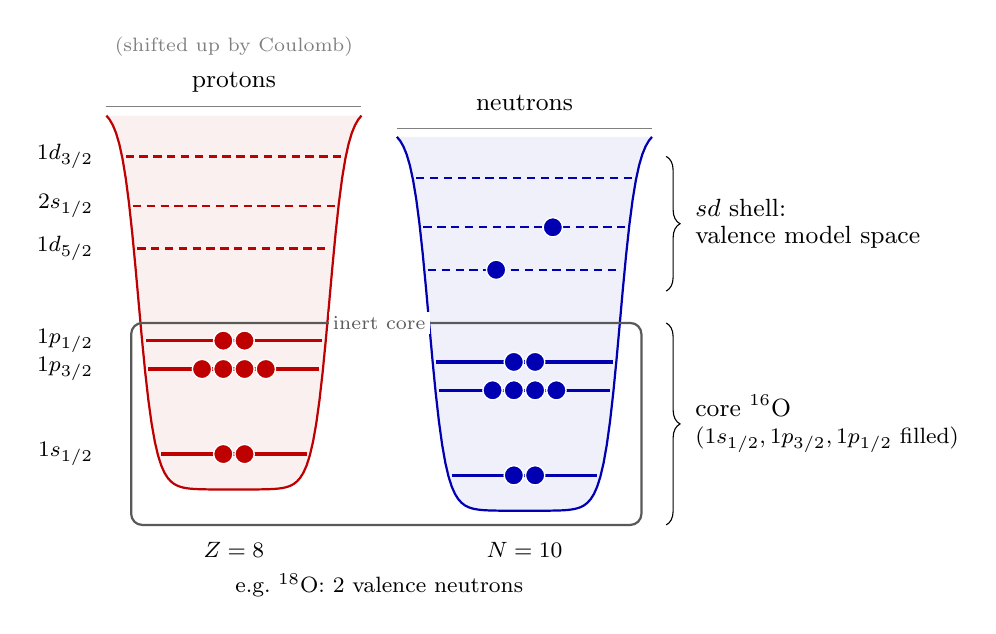
\begin{tikzpicture}[scale=0.9,
    declare function={hw(\y,\t)=1.35+0.12*ln(5.4/(\t-\y)-1);},
    pnuc/.style={circle,fill=red!75!black,draw=white,line width=0.5pt,inner sep=0pt,minimum size=7pt},
    nnuc/.style={circle,fill=blue!70!black,draw=white,line width=0.5pt,inner sep=0pt,minimum size=7pt}]
  \foreach \cx/\s/\col/\nuc/\t/\b in {1.2/0.3/red!75!black/pnuc/protons/{Z=8}, 5.3/0/blue!70!black/nnuc/neutrons/{N=10}} {
    \pgfmathsetmacro{\top}{1.3+\s}
    % schematic Woods--Saxon well
    \fill[\col!6!white,domain=-1.8:1.8,samples=80,variable=\x]
       plot ({\cx+\x},{\top-5.4/(1+exp((abs(\x)-1.35)/0.12))}) -- cycle;
    \draw[\col,thick,domain=-1.8:1.8,samples=80,variable=\x]
       plot ({\cx+\x},{\top-5.4/(1+exp((abs(\x)-1.35)/0.12))});
    \draw[gray] (\cx-1.8,\top) -- (\cx+1.8,\top);
    \node[font=\small] at (\cx,\top+0.35) {\t};
    \node[font=\footnotesize] at (\cx,-4.65) {$\b$};
    % core orbits (filled)
    \foreach \y/\d in {-3.6/2, -2.4/4, -2.0/2} {
      \pgfmathsetmacro{\yy}{\y+\s}\pgfmathsetmacro{\w}{hw(\yy,\top)-0.05}
      \draw[very thick,\col] (\cx-\w,\yy) -- (\cx+\w,\yy);
      \foreach \k in {1,...,\d} \node[\nuc] at ({\cx+0.3*(\k-(\d+1)/2)},\yy) {};
    }
    % sd valence orbits (empty)
    \foreach \y in {-0.7,-0.1,0.6} {
      \pgfmathsetmacro{\yy}{\y+\s}\pgfmathsetmacro{\w}{hw(\yy,\top)-0.05}
      \draw[thick,\col,densely dashed] (\cx-\w,\yy) -- (\cx+\w,\yy);
    }
  }
  % border around the inert core
  \draw[black!65,thick,rounded corners=4pt] (-0.25,-4.3) rectangle (6.95,-1.45);
  \node[font=\scriptsize,black!65,fill=white,inner sep=1.5pt] at (3.25,-1.45) {inert core};
  \node[font=\scriptsize,gray,align=center] at (1.2,2.45) {(shifted up by Coulomb)};
  \foreach \y/\lab in {-3.6/1s_{1/2}, -2.4/1p_{3/2}, -2.0/1p_{1/2}, -0.7/1d_{5/2}, -0.1/2s_{1/2}, 0.6/1d_{3/2}}
    \node[left,font=\footnotesize] at (-0.65,\y+0.3) {$\lab$};
  \node[nnuc] at (4.9,-0.7) {};
  \node[nnuc] at (5.7,-0.1) {};
  \draw[decorate,decoration={brace,amplitude=5pt}] (7.3,0.9) -- (7.3,-1.0)
     node[midway,right=7pt,align=left,font=\small] {$sd$ shell:\\[-1pt]valence model space};
  \draw[decorate,decoration={brace,amplitude=5pt}] (7.3,-1.45) -- (7.3,-4.3)
     node[midway,right=7pt,align=left,font=\small] {core ${}^{16}$O\\[-1pt]{\footnotesize ($1s_{1/2},1p_{3/2},1p_{1/2}$ filled)}};
  \node[font=\footnotesize] at (3.25,-5.15) {e.g.\ ${}^{18}$O: 2 valence neutrons};
\end{tikzpicture}
\end{center}
Two-particle basis: $\ket{(n_1\ell_1)j_1\,(n_2\ell_2)j_2;JM}$.
\[
\begin{array}{ll}
J^\pi=0^+: & \ket{(1d_{5/2})^2,J{=}0},\ \ket{(1d_{3/2})^2,J{=}0},\ \ket{(2s_{1/2})^2,J{=}0},\\[1mm]
J^\pi=1^+: & \ket{(1d_{3/2})(2s_{1/2}),J{=}1},\ \dots\\[1mm]
J^\pi=2^+: & \ket{(1d_{5/2})^2,J{=}2},\ \ket{(1d_{3/2})^2,J{=}2},\ \ket{(1d_{5/2})(1d_{3/2}),J{=}2},\\
           & \ket{(1d_{5/2})(2s_{1/2}),J{=}2},\ \ket{(1d_{3/2})(2s_{1/2}),J{=}2},\\[1mm]
J^\pi=3^+: & \ket{(1d_{5/2})(2s_{1/2}),J{=}3},\ \ket{(1d_{5/2})(1d_{3/2}),J{=}3},\\[1mm]
J^\pi=4^+: & \ket{(1d_{5/2})^2,J{=}4},\ \dots
\end{array}
\]
using $\frac52\otimes\frac32=1,2,3,4$; $\frac52\otimes\frac12=2,3$; $\frac32\otimes\frac12=1,2$; $(\frac52)^2=0,2,4$; $(\frac32)^2=0,2$.

$\Rightarrow$ diagonalisation of $\op H$ in the basis of 2-particle states for each $J,\pi$ ($J$-scheme): configuration mixing due to $\op V$ $\Rightarrow$ \textbf{interacting shell model}.

E.g.\ for $J^\pi=0^+$ the dimension is 3:
\[
\ket1=\ket{(1d_{5/2})^2,0},\qquad \ket2=\ket{(1d_{3/2})^2,0},\qquad \ket3=\ket{(2s_{1/2})^2,0},
\]
\[
\op H=\op h(1)+\op h(2)+\op V(1,2),\qquad
\braket{i|\op h|i}=\varepsilon_i,\qquad \braket{i|\op h(1)+\op h(2)|i}=2\varepsilon_i,
\]
\[
H_{ij}=\braket{i|\op H|j},\quad \braket{i|\op V|j}=V_{ij},
\]
\[
\begin{pmatrix}
2\varepsilon_{1d_{5/2}}+V_{11} & V_{12} & V_{13}\\
V_{21} & 2\varepsilon_{1d_{3/2}}+V_{22} & V_{23}\\
V_{31} & V_{32} & 2\varepsilon_{2s_{1/2}}+V_{33}
\end{pmatrix}
\begin{pmatrix}c_1\\c_2\\c_3\end{pmatrix}
\overset{!}{=}E\begin{pmatrix}c_1\\c_2\\c_3\end{pmatrix}.
\]
How to determine $\op V$ --- the effective interaction?
\begin{itemize}
\item $\varepsilon_i$, $V_{ij}$ $\to$ free parameters $\to$ fit to known properties of e.g.\ stable nuclei $\to$ predictions for other systems;
\item or calculation of the effective interaction from a realistic bare $NN$ force.
\end{itemize}
One can construct more complicated configurations $\to$ $n$ valence particles. If $V$ is 2-body, \emph{the matrix elements of $n$-particle configurations can be expressed as linear combinations of 2-body matrix elements.} The dimension of the space grows drastically $\Rightarrow$ large-scale diagonalisation.

%--- 18O with the USD interaction ---
\paragraph{Example: ${}^{18}$O with the USD interaction.}
A widely used empirical effective interaction for the $sd$ shell is the USD (``universal $sd$'') interaction of Wildenthal (B.~H.~Wildenthal, Prog.\ Part.\ Nucl.\ Phys.\ \textbf{11}, 5 (1984); see also B.~A.~Brown, B.~H.~Wildenthal, Annu.\ Rev.\ Nucl.\ Part.\ Sci.\ \textbf{38}, 29 (1988)). It consists of 3 single-particle energies and 63 two-body matrix elements $\braket{ab;JT|\op V|cd;JT}$, treated as free parameters and fitted to 447 measured energy levels of $sd$-shell nuclei with $A=17$--$39$ (rms deviation about 150~keV). The two-body matrix elements are scaled with the mass number as $(18/A)^{0.3}$. The single-particle energies are
\[
\varepsilon_{1d_{5/2}}=-3.95~\text{MeV},\qquad
\varepsilon_{2s_{1/2}}=-3.16~\text{MeV},\qquad
\varepsilon_{1d_{3/2}}=+1.65~\text{MeV},
\]
close to the measured $5/2^+$, $1/2^+$ and $3/2^+$ states of ${}^{17}$O relative to ${}^{16}$O$+n$ ($-4.14$, $-3.27$ and $+0.94$~MeV).

For ${}^{18}$O (two valence neutrons, $T=1$) the $0^+$ matrix above becomes, in MeV and in the basis $\ket{(1d_{5/2})^2}$, $\ket{(1d_{3/2})^2}$, $\ket{(2s_{1/2})^2}$,
\[
H(0^+)=
\begin{pmatrix}
-10.72 & -3.19 & -1.33\\
-3.19 & 1.11 & -1.08\\
-1.33 & -1.08 & -8.45
\end{pmatrix},
\qquad E_{0^+_1}=-12.17~\text{MeV},
\]
with $|c_1|^2=0.79$, $|c_2|^2=0.06$, $|c_3|^2=0.15$. The residual interaction lowers the ground state by more than 4~MeV with respect to the unperturbed $2\varepsilon_{1d_{5/2}}=-7.90$~MeV (pairing), and the energy relative to ${}^{16}$O$+2n$ agrees with the measured value $B({}^{16}\mathrm{O})-B({}^{18}\mathrm{O})=-12.19$~MeV (AME2020 masses).

The other $J^\pi$ blocks are constructed in the same way. The USD matrices for ${}^{18}$O are (in MeV; the signs of the off-diagonal elements depend on the phase convention of the two-particle states):

$J^\pi=1^+$, basis $\ket{(1d_{3/2})(2s_{1/2})}$, $\ket{(1d_{5/2})(1d_{3/2})}$,
\[
H(1^+)=
\begin{pmatrix}
-0.91 & 0.19\\
0.19 & -1.27
\end{pmatrix},
\qquad E=-1.35,\ -0.83;
\]
$J^\pi=2^+$, basis $\ket{(1d_{5/2})^2}$, $\ket{(1d_{3/2})^2}$, $\ket{(1d_{5/2})(1d_{3/2})}$, $\ket{(1d_{5/2})(2s_{1/2})}$, $\ket{(1d_{3/2})(2s_{1/2})}$,
\[
H(2^+)=
\begin{pmatrix}
-8.90 & -1.62 & -0.28 & -0.86 & 0.62\\
-1.62 & 3.23 & -0.61 & -0.40 & 0.52\\
-0.28 & -0.61 & -2.63 & -0.48 & 0.52\\
-0.86 & -0.40 & -0.48 & -7.93 & 1.94\\
0.62 & 0.52 & 0.52 & 1.94 & -1.92
\end{pmatrix},
\]
\[
E=-9.99,\ -7.73,\ -2.71,\ -1.24,\ 3.52;
\]
$J^\pi=3^+$, basis $\ket{(1d_{5/2})(2s_{1/2})}$, $\ket{(1d_{5/2})(1d_{3/2})}$,
\[
H(3^+)=
\begin{pmatrix}
-6.35 & -0.67\\
-0.67 & -1.71
\end{pmatrix},
\qquad E=-6.44,\ -1.62;
\]
$J^\pi=4^+$, basis $\ket{(1d_{5/2})^2}$, $\ket{(1d_{5/2})(1d_{3/2})}$,
\[
H(4^+)=
\begin{pmatrix}
-8.06 & -1.24\\
-1.24 & -3.75
\end{pmatrix},
\qquad E=-8.39,\ -3.42.
\]
The diagonal elements are $\varepsilon_a+\varepsilon_b+\braket{ab;J|\op V|ab;J}$. The configuration mixing differs strongly between the blocks: the $4^+_1$ state is 93\,\% $(1d_{5/2})^2$ and the $3^+_1$ state 98\,\% $(1d_{5/2})(2s_{1/2})$, whereas the $2^+_1$ state is a strongly mixed state with 61\,\% $(1d_{5/2})^2$ and 32\,\% $(1d_{5/2})(2s_{1/2})$, because the two unperturbed configurations lie only 1~MeV apart. Note also that the $J=1$ and $J=3$ blocks contain no $(1d_{5/2})^2$, $(2s_{1/2})^2$ or $(1d_{3/2})^2$ components: for two identical nucleons in the same $j$ shell only even $J$ are allowed.
The eigenvalues $E$ (relative to ${}^{16}$O$+2n$) of all blocks together form the spectrum shown in Fig.~\ref{fig:O18USD}. The yrast $2^+$, $4^+$ and the $3^+$ state are reproduced within a few hundred keV. Experimentally there are two $0^+$ states (3.63 and 5.34~MeV) and two $2^+$ states (3.92 and 5.25~MeV) where the $sd$ model space gives only one of each. The additional states are mainly deformed $4p$-$2h$ configurations (two nucleons excited from the $p$ shell of the ${}^{16}$O core), which lie outside the model space and mix with the $sd$ states (R.~D.~Lawson, F.~J.~D.~Serduke, H.~T.~Fortune, Phys.\ Rev.\ C \textbf{14}, 1245 (1976)).

The same interaction, without any change of its parameters, can be applied to more valence nucleons; for $n$ particles the Hamiltonian matrix is built from the same $\varepsilon_a$ and two-body matrix elements (scaled by $(18/A)^{0.3}$), in a basis of $n$-particle Slater determinants (the $M$-scheme). Fig.~\ref{fig:O18USD} shows ${}^{19}$O and ${}^{20}$O (3 and 4 valence neutrons, $M$-scheme dimensions 37 and 81). The ground-state energies relative to ${}^{16}$O are $-16.06$ and $-23.83$~MeV, compared with the measured $-16.14$ and $-23.75$~MeV, and the low-lying levels are reproduced to typically 0.2--0.3~MeV. In ${}^{19}$O the $5/2^+$ ground state, the almost degenerate $3/2^+$ state (0.10~MeV) and the $9/2^+$ state (2.37~MeV) are dominated by the $(1d_{5/2})^3$ configuration, which for three neutrons allows $J=3/2,\,5/2,\,9/2$; the $1/2^+$ state (1.47~MeV) is mainly $(1d_{5/2})^2_{0}\,2s_{1/2}$. In ${}^{20}$O the $0^+$, $2^+$, $4^+$ sequence resembles that of ${}^{18}$O, with the core-excited intruder states no longer appearing at low energy.
\begin{figure}[ht]
\centering
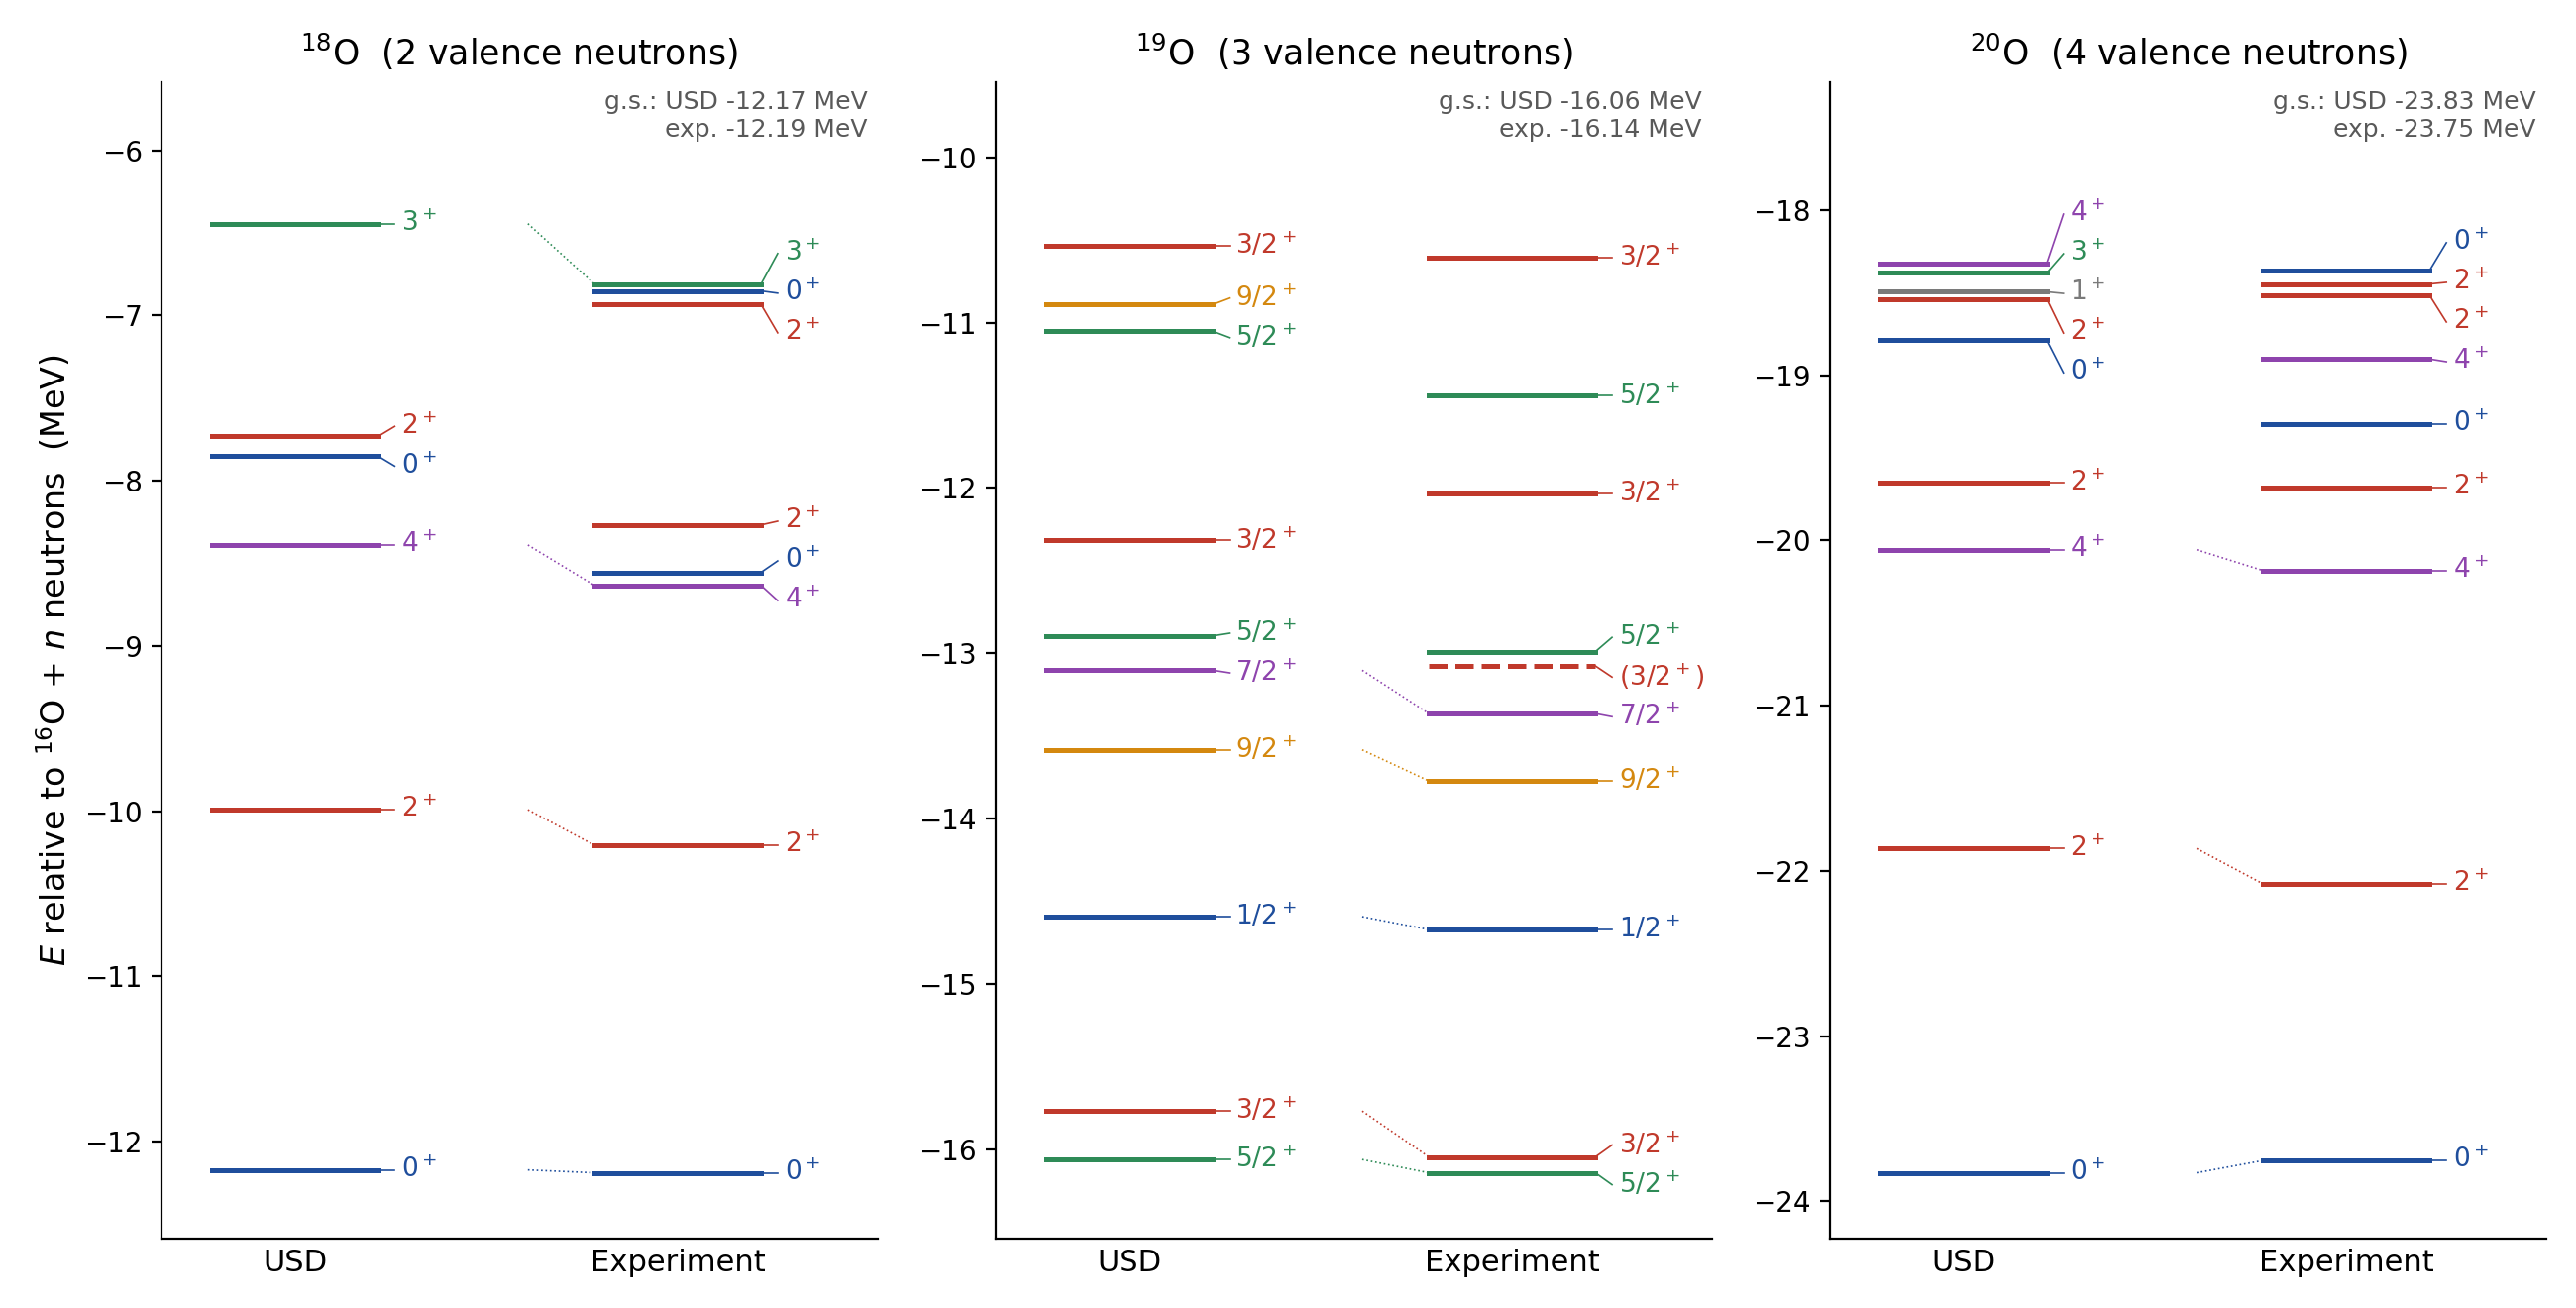
\includegraphics[width=\linewidth]{oxygen_usd.png}
\caption{Positive-parity spectra of ${}^{18}$O, ${}^{19}$O and ${}^{20}$O (2, 3 and 4 valence neutrons): shell-model calculation in the $sd$ shell with the same USD single-particle energies and two-body matrix elements (B.~H.~Wildenthal, Prog.\ Part.\ Nucl.\ Phys.\ \textbf{11}, 5 (1984)), compared with experiment (ENSDF; evaluations D.~R.~Tilley \emph{et al.}, Nucl.\ Phys.\ A \textbf{595}, 1 (1995) for $A=18$, 19 and D.~R.~Tilley \emph{et al.}, Nucl.\ Phys.\ A \textbf{636}, 249 (1998) for $A=20$). Energies are given relative to ${}^{16}$O plus the valence neutrons, the experimental ground-state energies are from the AME2020 mass evaluation (M.~Wang \emph{et al.}, Chin.\ Phys.\ C \textbf{45}, 030003 (2021)). Experimental levels with a tentative spin are dashed; dotted lines connect the lowest state of each $J^\pi$.}
\label{fig:O18USD}
\end{figure}

\subsection{Schematic interaction: \texorpdfstring{$\delta$}{delta}-force}
Some schematic interactions can provide a useful insight into the many-body problem. Let us assume
\[
V(\vec r_1,\vec r_2)=-V_0\,\delta(\vec r_1-\vec r_2).
\]
For simplicity we do not consider spin and assume a single spherical $\ell$-shell $\ket{n\ell m}$, $\vec L=\vec\ell_1+\vec\ell_2$:
\[
\Psi_{\ell^2,LM}=R_{n\ell}(r_1)R_{n\ell}(r_2)\sum_{m,m'}\big(\ell m\,\ell m'\big|LM\big)\,Y_{\ell m}(\vartheta_1,\varphi_1)\,Y_{\ell m'}(\vartheta_2,\varphi_2),
\qquad E=E_0+\Delta E,
\]
\[
\Delta E=\braket{\ell^2,LM|-V_0\,\delta(\vec r_1-\vec r_2)|\ell^2,LM}
\]
\[
=-V_0\int_0^\infty r_1^2\ud r_1\int_0^\infty r_2^2\ud r_2\int_0^\pi\sin\vartheta_1\ud\vartheta_1\int_0^\pi\sin\vartheta_2\ud\vartheta_2\int_0^{2\pi}\ud\varphi_1\int_0^{2\pi}\ud\varphi_2
\]
\[
\times\sum_{\substack{m,m'\\ \mu,\mu'}}\big(\ell m\,\ell m'\big|LM\big)\big(\ell\mu\,\ell\mu'\big|LM\big)
R_{n\ell}(r_1)R_{n\ell}(r_2)\,Y^*_{\ell m}(\vartheta_1,\varphi_1)Y^*_{\ell m'}(\vartheta_2,\varphi_2)
\]
\[
\times\frac{\delta(r_1-r_2)\,\delta(\vartheta_1-\vartheta_2)\,\delta(\varphi_1-\varphi_2)}{r_1^2\sin\vartheta_1}
\]
\[
\times R_{n\ell}(r_1)R_{n\ell}(r_2)\,Y_{\ell\mu}(\vartheta_1,\varphi_1)Y_{\ell\mu'}(\vartheta_2,\varphi_2)
=-V_0\int_0^\infty r^2\big(R_{n\ell}(r)\big)^4\ud r\cdot I,
\]
\[
I=\sum_{\substack{m,m'\\ \mu,\mu'}}\big(\ell m\,\ell m'\big|LM\big)\big(\ell\mu\,\ell\mu'\big|LM\big)\int_0^\pi\sin\vartheta\,\ud\vartheta\int_0^{2\pi}\ud\varphi\;Y^*_{\ell m}Y^*_{\ell m'}Y_{\ell\mu}Y_{\ell\mu'} .
\]
Because
\[
Y_{\ell m}(\vartheta,\varphi)\,Y_{\ell m'}(\vartheta,\varphi)=\sum_{L',M'}\frac{2\ell+1}{\sqrt{4\pi(2L'+1)}}\big(\ell m\,\ell m'\big|L'M'\big)\big(\ell0\,\ell0\big|L'0\big)\,Y_{L'M'}(\vartheta,\varphi),
\]
we get
\[
I=\sum_{\substack{L_1M_1\\L_2M_2}}\sum_{\substack{m,m'\\ \mu,\mu'}}\big(\ell m\,\ell m'\big|LM\big)\big(\ell\mu\,\ell\mu'\big|LM\big)\frac{(2\ell+1)^2}{4\pi\sqrt{(2L_1+1)(2L_2+1)}}\big(\ell m\,\ell m'\big|L_1M_1\big)\big(\ell0\,\ell0\big|L_10\big)
\]
\[
\times\big(\ell\mu\,\ell\mu'\big|L_2M_2\big)\big(\ell0\,\ell0\big|L_20\big)
\underbrace{\int_0^\pi\sin\vartheta\,\ud\vartheta\int_0^{2\pi}\ud\varphi\;Y^*_{L_1M_1}Y_{L_2M_2}}_{\delta_{L_1L_2}\delta_{M_1M_2}}
\]
\[
=\sum_{L_1M_1}\frac{(2\ell+1)^2}{4\pi(2L_1+1)}\big(\ell0\,\ell0\big|L_10\big)^2
\underbrace{\sum_{m,m'}\big(\ell m\,\ell m'\big|LM\big)\big(\ell m\,\ell m'\big|L_1M_1\big)}_{\delta_{LL_1}\delta_{MM_1}}
\underbrace{\sum_{\mu,\mu'}\big(\ell\mu\,\ell\mu'\big|LM\big)\big(\ell\mu\,\ell\mu'\big|L_1M_1\big)}_{\delta_{LL_1}\delta_{MM_1}}
\]
\[
=\frac{(2\ell+1)^2}{4\pi(2L+1)}\big(\ell0\,\ell0\big|L0\big)^2=\frac{(2\ell+1)^2}{4\pi}\begin{pmatrix}\ell&\ell&L\\0&0&0\end{pmatrix}^2,
\]
where we used the 3$j$ symbol
\[
\begin{pmatrix}j_1&j_2&j_3\\m_1&m_2&m_3\end{pmatrix}=\frac{(-1)^{j_1-j_2-m_3}}{\sqrt{2j_3+1}}\big(j_1m_1\,j_2m_2\big|j_3\,{-m_3}\big).
\]
Hence
\[
\Delta E(\ell^2,L)=-V_0\int_0^\infty r^2\big(R_{n\ell}(r)\big)^4\ud r\cdot\frac{(2\ell+1)^2}{4\pi}\begin{pmatrix}\ell&\ell&L\\0&0&0\end{pmatrix}^2,
\]
\[
\boxed{\Delta E(\ell^2,L)=(2\ell+1)^2\,F_0\begin{pmatrix}\ell&\ell&L\\0&0&0\end{pmatrix}^2},
\qquad
F_0=-\frac{V_0}{4\pi}\int_0^\infty r^2\big(R_{n\ell}(r)\big)^4\ud r .
\]
Values of the squared 3$j$ symbol (it vanishes for odd $L$):
\begin{center}
\begin{tabular}{c c c}
$L$ & $g$ shell, $\ell=4$ & $h$ shell, $\ell=5$\\ \hline
0 & 0.111 & 0.091\\
1 & 0 & 0\\
2 & 0.0289 & 0.0233\\
3 & 0 & 0\\
4 & 0.0180 & 0.0140\\
6 & 0.0155 & 0.0110\\
8 & 0.0224 & 0.0106\\
10 & --- & 0.0164
\end{tabular}
\end{center}
The $L=0$ state is strongly favoured (lowered), the other states are shifted much less. The $\delta$ interaction is a simple effective force describing \textbf{pairing} in nuclei.

\subsection{Pairing}
There are many experimental observables indicating that pairing of nucleons with opposite spins occurs in nuclei:
\begin{itemize}
\item odd-even staggering of separation energies (if there is a pair of nucleons, this leads to an extra binding energy compared to an unpaired system);
\item spins of all even-even nuclei in the ground state are 0;
\item spectra of core $+$ 2 nucleons of the same kind show a ``gap'' between the $0^+$ ground state and the $2^+,4^+,6^+,\dots$ states:
\end{itemize}
\begin{center}
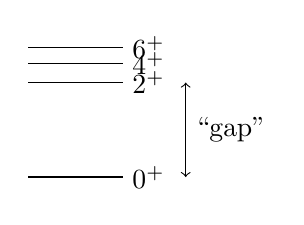
\begin{tikzpicture}[scale=0.8]
\draw (0,0) -- (1.5,0) node[right]{$0^+$};
\draw (0,1.5) -- (1.5,1.5) node[right]{$2^+$};
\draw (0,1.8) -- (1.5,1.8) node[right]{$4^+$};
\draw (0,2.05) -- (1.5,2.05) node[right]{$6^+$};
\draw[<->] (2.5,0) -- (2.5,1.5) node[midway,right]{``gap''};
\end{tikzpicture}
\end{center}
Let us assume pairs of states $\ket{n\ell jm}$, $\ket{n\ell j\,{-m}}$, which have the largest spatial overlap:
\[
\ket{j^2,J{=}0}=\sum_m\big(jm\,j\,{-m}\big|00\big)\ket{n\ell jm}\ket{n\ell j\,{-m}}
=\sum_m(-1)^{j-m}\frac{1}{\sqrt{2j+1}}\ket{n\ell jm}\ket{n\ell j\,{-m}}
\]
\[
=\frac{1}{\sqrt{2j+1}}\sum_m\ket{n\ell jm}\widetilde{\ket{n\ell jm}}\quad\text{(``Cooper pair'')},
\]
with the time-reversed state
\[
\widetilde{\ket{n\ell jm}}=(-1)^{j-m}\ket{n\ell j\,{-m}} .
\]
More generally, we can construct a correlated wave function from Cooper pairs, e.g.\ for ${}^{210}$Po $=2p+{}^{208}$Pb
\[
\ket{{}^{210}\text{Po};0^+_1}\approx c_1\ket{(1h_{9/2})^2,0}+c_2\ket{(2f_{7/2})^2,0}+c_3\ket{(1i_{13/2})^2,0}+\dots
\]
This leads to a smoothing of the Fermi surface: the ``occupation'' $n$ of the levels changes smoothly around $\varepsilon_F$ instead of a sharp step.
\begin{center}
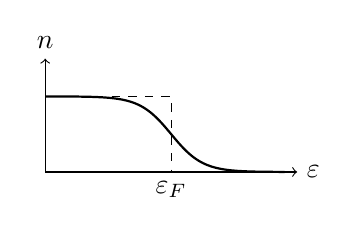
\begin{tikzpicture}[scale=0.8]
\draw[->] (0,0) -- (4,0) node[right]{$\varepsilon$};
\draw[->] (0,0) -- (0,1.8) node[above]{$n$};
\draw[dashed] (0,1.2) -- (2,1.2) -- (2,0);
\draw[thick,domain=0:3.8,samples=60,smooth] plot (\x,{1.2/(1+exp((\x-2)/0.25))});
\node[below] at (2,0) {$\varepsilon_F$};
\end{tikzpicture}
\end{center}
Pairing of nucleons of the same kind ($pp$, $nn$) plays an important role in nuclear structure ($pn$ pairing is small, because in heavy nuclei protons and neutrons occupy different orbits).

Schematic picture of the spectrum of an even-even nucleus:
\begin{center}
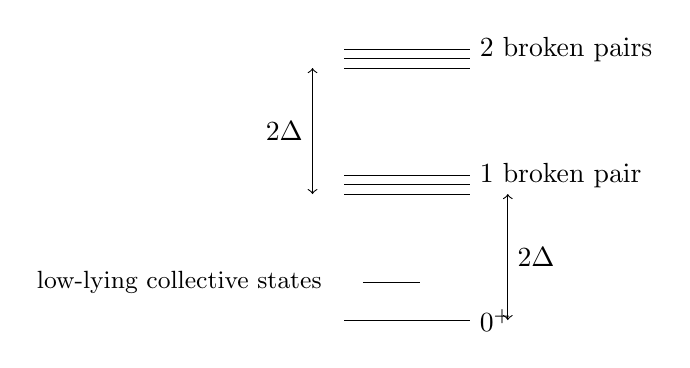
\begin{tikzpicture}[scale=0.8]
\draw (0,0) -- (2,0) node[right]{$0^+$};
\draw (0.3,0.6) -- (1.2,0.6);
\node[left] at (-0.2,0.6) {\small low-lying collective states};
\draw (0,2) -- (2,2); \draw (0,2.15) -- (2,2.15); \draw (0,2.3) -- (2,2.3) node[right]{1 broken pair};
\draw[<->] (2.6,0) -- (2.6,2) node[midway,right]{$2\Delta$};
\draw (0,4) -- (2,4); \draw (0,4.15) -- (2,4.15); \draw (0,4.3) -- (2,4.3) node[right]{2 broken pairs};
\draw[<->] (-0.5,2) -- (-0.5,4) node[midway,left]{$2\Delta$};
\end{tikzpicture}
\end{center}
$\Delta$ is the pairing gap,
\[
2\Delta\approx\frac{12}{\sqrt A}\ \text{MeV}.
\]
Pairing correlations can be effectively treated in the BCS (Bardeen--Cooper--Schrieffer) theory. (BCS theory describes superconductivity $\to$ pairing of electrons with opposite momenta.)

%=====================================================================
\section{Electromagnetic transitions (simplified approach)}
%=====================================================================
Let us assume a system described by the Hamiltonian
\[
\op H=\op H_0+\op H_{\rm int}(t),
\]
where $\op H_0$ describes an unperturbed microsystem (nucleus) and $\op H_{\rm int}$ is a periodic perturbation representing a photon with energy $\hbar\omega$,
\[
\op H_{\rm int}=\op B\,e^{-i\omega t}+\op B^\dagger e^{i\omega t}.
\]
The interaction causes transitions from the initial state $\ket i$ ($\op H_0\ket i=E_i\ket i$) to the final state $\ket f$ ($\op H_0\ket f=E_f\ket f$). The transition probability (per unit time) in the 1st order of time-dependent perturbation theory is given by
\begin{itemize}
\item absorption ($E_f=E_i+\hbar\omega$):
\[
w_{i\to f}=\frac{2\pi}{\hbar}\,\delta(E_f-E_i-\hbar\omega)\,\big|\braket{f|\op B|i}\big|^2 ,
\]
\item emission ($E_f=E_i-\hbar\omega$):
\[
w_{i\to f}=\frac{2\pi}{\hbar}\,\delta(E_f-E_i+\hbar\omega)\,\big|\braket{f|\op B^\dagger|i}\big|^2
\]
\end{itemize}
(see e.g.\ P.~Cejnar, lecture notes on quantum mechanics).
% TODO: check the reference -- handwritten "Cejnar: QM 15?"

The photon can be represented by a vector field
\[
\vec A_{\tau,\vec k}=A_0\,\vec\xi_\tau\,e^{i(\vec k\cdot\vec r-\omega t)}+A_0\,\vec\xi^{\,*}_\tau\,e^{-i(\vec k\cdot\vec r-\omega t)},
\]
where $\vec k$ is the wave vector and $\tau=\pm1$ the polarisation,
\[
\vec\xi_{\tau=\pm1}=\mp\frac{1}{\sqrt2}\big(\vec e_x\pm i\vec e_y\big).
\]
$\vec A$ is a solution of the Maxwell equations without sources. Without charges $\varphi=0$, and the Lorenz gauge $\vec\nabla\cdot\vec A+\frac{1}{c^2}\frac{\partial\varphi}{\partial t}=0$ gives $\vec\nabla\cdot\vec A=0$ $\Rightarrow$ $\vec k\cdot\vec A=0$ $\Rightarrow$ $\vec k\perp\vec A$ ($\tau=0$ for real photons is not possible).

The nucleus is described by the (charge) density $\rho_n(\vec r)$ and current $\vec j_n(\vec r)$. The interaction of the nucleus with the electromagnetic field is given by the interaction Hamiltonian
\[
\op H_{\rm int}=\int\ud^3r\,\big[\rho_n\varphi-\vec j_n\cdot\vec A\big],
\]
which for $\varphi=0$ takes the simpler form
\[
\op H_{\rm int}=-\int\ud^3r\,\vec j_n(\vec r)\cdot\vec A(\vec r,t)
\quad\Rightarrow\quad
\op H_{\rm int}=\underbrace{-A_0\int\ud^3r\,\vec\xi_\tau\cdot\vec j_n\,e^{i\vec k\cdot\vec r}}_{\op B}\,e^{-i\omega t}
\]
\[
\qquad\ \underbrace{-A_0\int\ud^3r\,\vec\xi^{\,*}_\tau\cdot\vec j_n\,e^{-i\vec k\cdot\vec r}}_{\op B^\dagger}\,e^{i\omega t},
\]
where $A_0$ is the normalisation (in a box of size $L$), $A_0=\sqrt{\hbar/(2\varepsilon_0L^3\omega)}$.
For absorption we have
\[
w_{i\to f}=\frac{2\pi}{\hbar}\,\delta(E_f-E_i-\hbar\omega)\,\big|\braket{f|\op B|i}\big|^2 .
\]
The quantity to be calculated is the matrix element
\[
\braket{f|\op B|i}=-A_0\Big\langle f\Big|\int\ud^3r\,\vec j_n\cdot\vec\xi_\tau\,e^{i\vec k\cdot\vec r}\Big|i\Big\rangle .
\]
For the nuclear density and current
\[
\rho(\vec r)=\sum_{j=1}^Ae_j\,\delta(\vec r-\vec r_j),\qquad
\vec j(\vec r)=\sum_{j=1}^A\frac{e_j}{m_j}\,\delta(\vec r-\vec r_j)\,\vec p_j ,
\]
so that, using the Taylor expansion of the plane wave $e^{i\vec k\cdot\vec r}\approx1+i\vec k\cdot\vec r+\dots$ ($kr\ll1$),
\[
\braket{f|\op B|i}=-A_0\Big\langle f\Big|\sum_{j=1}^A\frac{e_j}{m_j}\,\vec p_j\cdot\vec\xi_\tau\,e^{i\vec k\cdot\vec r_j}\Big|i\Big\rangle
\approx-A_0\Big\langle f\Big|\sum_{j=1}^A\frac{e_j}{m_j}\,\vec p_j\cdot\vec\xi_\tau\,\big(1+i\vec k\cdot\vec r_j\big)\Big|i\Big\rangle .
\]

\paragraph{The first term:} $e^{i\vec k\cdot\vec r}\approx1$. Using $\frac{\vec p}{m}=\dot{\vec r}=\frac{1}{i\hbar}[\vec r,\op H_0]$, where $\op H_0$ is the nuclear Hamiltonian ($\op H_0\ket i=E_i\ket i$, $\op H_0\ket f=E_f\ket f$, $E_f-E_i=\hbar\omega$),
\[
\Big\langle f\Big|\sum_{j=1}^A\frac{e_j}{m_j}\,\vec p_j\cdot\vec\xi_\tau\Big|i\Big\rangle
=\frac{1}{i\hbar}\Big\langle f\Big|\sum_{j=1}^Ae_j\,\underbrace{[\vec r_j,\op H_0]}_{\vec r_j\op H_0-\op H_0\vec r_j}\cdot\vec\xi_\tau\Big|i\Big\rangle
=\frac{i}{\hbar}\Big\langle f\Big|\sum_{j=1}^Z e\,\vec r_j\cdot\vec\xi_\tau\Big|i\Big\rangle(E_f-E_i)
\]
\[
=\frac{i}{\hbar}\braket{f|\op{\vec D}\cdot\vec\xi_\tau|i}\,\hbar\omega,
\qquad
\op{\vec D}=\sum_{j=1}^Ze\,\vec r_j\qquad\text{(dipole approximation)}.
\]

\paragraph{The second term:}
\[
\Big\langle f\Big|\sum_{j=1}^Ae_j\Big(\frac{\vec p_j}{m_j}\cdot\vec\xi_\tau\Big)\big(i\vec k\cdot\vec r_j\big)\Big|i\Big\rangle .
\]
We decompose
\[
(\vec p\cdot\vec\xi)(\vec k\cdot\vec r)
=\frac12\underbrace{\big[(\vec\xi\cdot\vec p)(\vec k\cdot\vec r)+(\vec\xi\cdot\vec r)(\vec k\cdot\vec p)\big]}_{F_+}
+\frac12\underbrace{\big[(\vec\xi\cdot\vec p)(\vec k\cdot\vec r)-(\vec\xi\cdot\vec r)(\vec k\cdot\vec p)\big]}_{F_-}
=\tfrac12F_++\tfrac12F_- .
\]
For $F_+$:
\[
F_+=m\big[(\vec\xi\cdot\dot{\vec r})(\vec k\cdot\vec r)+(\vec\xi\cdot\vec r)(\vec k\cdot\dot{\vec r})\big]
=m\frac{\ud}{\ud t}\big[(\vec\xi\cdot\vec r)(\vec k\cdot\vec r)\big]
=m\sum_{i,j}\xi_ik_j\frac{\ud}{\ud t}(r_ir_j)
\]
\[
=m\sum_{i,j}\xi_ik_j\frac{\ud}{\ud t}\Big(r_ir_j-\frac13\delta_{ij}r^2\Big)
=\frac{m}{3e}\sum_{i,j}\xi_ik_j\frac{\ud}{\ud t}Q_{ij}
=\frac{m}{3e}\,\vec\xi^{\,T}\dot Q\,\vec k ,
\]
where we could subtract $\frac13\sum_i\xi_ik_i\frac{\ud}{\ud t}r^2=0$, because $\vec k\cdot\vec\xi=0$ (since $\vec k\cdot\vec A=0$), and
\[
Q_{ij}=e\big(3r_ir_j-\delta_{ij}r^2\big)
\]
is the electric quadrupole moment. For $F_-$:
\[
F_-=(\vec\xi\cdot\vec p)(\vec k\cdot\vec r)-(\vec\xi\cdot\vec r)(\vec k\cdot\vec p)
=\big[\vec k\times\vec\xi\big]\cdot\big[\vec r\times\vec p\big]
=\underbrace{(\vec k\times\vec\xi)}_{\propto\vec B}\cdot\underbrace{\vec\ell}_{\propto\vec\mu},
\qquad \vec B=\vec\nabla\times\vec A .
\]
So for the second term we get
\[
i\Big\langle f\Big|\sum_je_j\Big(\frac{\vec p_j}{m_j}\cdot\vec\xi_\tau\Big)\big(\vec k\cdot\vec r_j\big)\Big|i\Big\rangle
=\frac i6\Big\langle f\Big|\sum_{j=1}^Z\vec\xi^{\,T}_\tau\dot{\op Q}\,\vec k\Big|i\Big\rangle
+\frac i2\big(\vec k\times\vec\xi_\tau\big)\cdot\Big\langle f\Big|\sum_{j=1}^Z\frac em\,\vec\ell_j\Big|i\Big\rangle ,
\]
\[
\dot{\op Q}=\frac{1}{i\hbar}\big[\op Q,\op H_0\big],
\]
\[
=-\frac{1}{6\hbar}\Big\langle f\Big|\sum_{j=1}^Z\vec\xi^{\,T}_\tau\op Q\,\vec k\Big|i\Big\rangle\underbrace{(E_f-E_i)}_{\hbar\omega}
+\underbrace{i\big(\vec k\times\vec\xi_\tau\big)}_{\sim\vec B_0}\cdot\Big\langle f\Big|\sum_{j=1}^Z\op{\vec\mu}_j\Big|i\Big\rangle,
\qquad \vec\mu_j=\frac{e\vec\ell_j}{2m},
\]
\[
=-\frac{1}{6\hbar}\,\vec\xi^{\,T}_\tau\braket{f|\op Q|i}\,\vec k\,(\hbar\omega)+\vec B_0\cdot\braket{f|\op{\vec\mu}|i},
\]
with the electric quadrupole moment and the (orbital part of the) magnetic dipole moment
\[
\op Q_{k\ell}=\sum_{j=1}^Ze\big(3r^k_jr^\ell_j-\delta_{k\ell}r_j^2\big),
\qquad
\op{\vec\mu}=\sum_{j=1}^Z\frac{e}{2m}\,\vec\ell_j .
\]
Altogether
\[
\braket{f|\op B|i}\approx\frac{iA_0}{\hbar}\braket{f|\op{\vec D}|i}\cdot\vec\xi_\tau\,\hbar\omega
-\frac{A_0}{6\hbar}\,\vec\xi^{\,T}_\tau\braket{f|\op Q|i}\,\vec k\,(\hbar\omega)
-iA_0\big(\vec k\times\vec\xi_\tau\big)\cdot\braket{f|\op{\vec\mu}|i}.
\]
If the states $\ket i$, $\ket f$ represent nuclear states with good $J$ and parity, not all terms can contribute simultaneously. E.g.\ if $\ket i=\ket{J^\pi=0^+}$:
\begin{itemize}
\item $\braket{f|\op{\vec D}|0^+}\neq0$ only for $J^\pi_f=1^-$ ($\op{\vec D}\to rY_{1\mu}$),
\item $\braket{f|\op Q|0^+}\neq0$ only for $J^\pi_f=2^+$ ($\op Q\to r^2Y_{2\mu}$),
\item $\braket{f|\op{\vec\mu}|0^+}\neq0$ only for $J^\pi_f=1^+$ ($\vec\ell$ is a pseudovector),
\end{itemize}
$\Rightarrow$ conservation of angular momentum and parity.

\subsection{Transition rates and reduced transition probabilities}
For absorption of a photon with wave vector $\vec k$ and polarisation $\tau$
\[
w_{i\to f}(\vec k,\tau)=\frac{2\pi}{\hbar}\,\delta(E_f-E_i-\hbar\omega)\,\big|\braket{f|\op B|i}\big|^2 ,
\]
and the cross section is
\[
\sigma(\hbar\omega,i\to f)=\frac12\sum_{\tau=\pm1}\sigma(\vec k,\tau,i\to f),
\qquad
\sigma(\vec k,\tau,i\to f)=\frac{w_{i\to f}(\vec k,\tau)}{\vec j_K},
\]
where $\vec j_K$ is the flux of incoming photons.
In the case of emission
\[
w_{i\to f}(\vec k,\tau)=\frac{2\pi}{\hbar}\,\delta(E_f-E_i+\hbar\omega)\,\big|\braket{f|\op B^\dagger|i}\big|^2 .
\]
Usually we are interested in the emission to all angles and polarisations
\[
T_{i\to f}(k)\equiv\sum_\tau\int w_{i\to f}(\vec k,\tau)\,\ud\Omega_k .
\]
Working with the plane-wave form of $\vec A$ is impractical in the expansion. One can use the expansion into \textbf{vector spherical harmonics}
\[
\vec Y_{LJM}\equiv\sum_{M\mu}\big(LM\,1\mu\big|JM\big)\,Y_{LM}\,\vec\xi_\mu ,
\]
where
\[
\op{\vec S}^2\vec\xi_\mu=1(1+1)\,\vec\xi_\mu,\qquad \op S_3\vec\xi_\mu=\mu\,\vec\xi_\mu,
\]
\[
\op{\vec S}^2\vec Y_{LJM}=1(1+1)\vec Y_{LJM},
\]
\[
\op{\vec L}^2\vec Y_{LJM}=L(L+1)\vec Y_{LJM},\qquad
\op{\vec J}^2\vec Y_{LJM}=J(J+1)\vec Y_{LJM},\qquad
\op J_3\vec Y_{LJM}=M\vec Y_{LJM}.
\]
One can show
\[
\vec\xi_\tau\,e^{i\vec k\cdot\vec r}=\sqrt{4\pi}\sum_{J=0}^\infty\sum_{L=|J-1|}^{J+1}i^L(2L+1)^{1/2}\,j_L(kr)\,\big(L0\,1\tau\big|J\tau\big)\,\vec Y_{LJ\tau}(\hat r),
\]
where $j_L$ are spherical Bessel functions. After a tedious derivation one can obtain
\[
T_{i\to f}(k\omega)=\frac{8\pi\alpha c}{e^2}\sum_\lambda\frac{(\hbar\omega)^{2\lambda+1}}{(\hbar c)^{2\lambda+1}\big[(2\lambda+1)!!\big]^2}\,\frac{\lambda+1}{\lambda}\,
\]
\[
\times\Big[\underbrace{B(E\lambda,i\to f)}_{\text{electric}}+\underbrace{B(M\lambda,i\to f)}_{\text{magnetic}}\Big],
\qquad \alpha=\frac{e^2}{4\pi\varepsilon_0\hbar c},
\]
where
\[
B(X\lambda,i\to f)=\frac{\big|\braket{f\|\op{\mathcal M}^X_\lambda\|i}\big|^2}{2J_i+1}
\]
is the \textbf{reduced transition probability} of type $X$ ($X=E$ electric, $X=M$ magnetic), $\op{\mathcal M}^X_\lambda$ is the multipole transition operator, and $\ket i\equiv\ket{\alpha_iJ_iM_i}$, $\ket f\equiv\ket{\alpha_fJ_fM_f}$. The reduced matrix element is defined by the Wigner--Eckart theorem
\[
\braket{\alpha_fJ_fM_f|\op{\mathcal M}^X_{\lambda\mu}|\alpha_iJ_iM_i}=\frac{1}{\sqrt{2J_f+1}}\big(J_iM_i\,\lambda\mu\big|J_fM_f\big)\braket{\alpha_fJ_f\|\op{\mathcal M}^X_\lambda\|\alpha_iJ_i}.
\]
Selection rules:
\[
|J_i-J_f|\le\lambda\le J_i+J_f ,
\]
\[
\text{electric operator:}\quad \pi_i\pi_f(-1)^\lambda=1,\qquad
\text{magnetic operator:}\quad \pi_i\pi_f(-1)^{\lambda+1}=1 .
\]
In the long-wave approximation ($kr\ll1$)
\[
\op{\mathcal M}^E_{\lambda\mu}=\int\rho\,r^\lambda\,Y_{\lambda\mu}\,\ud^3r,
\qquad
\op{\mathcal M}^M_{\lambda\mu}=\frac{1}{c(\lambda+1)}\int\big(\vec r\times\vec j\big)\cdot\vec\nabla\big(r^\lambda Y_{\lambda\mu}\big)\,\ud^3r .
\]
For point-like nucleons
\[
\op{\mathcal M}^E_{\lambda\mu}=\sum_{i=1}^Ae_i\,r_i^\lambda\,Y_{\lambda\mu}(\hat r_i),
\qquad
\op{\mathcal M}^M_{\lambda\mu}=\sum_{i=1}^A\Big\{g_s^i\,\vec s_i+\frac{2}{\lambda+1}\,g_\ell^i\,\vec\ell_i\Big\}\cdot\vec\nabla_i\big(r_i^\lambda Y_{\lambda\mu}(\hat r_i)\big),
\]
e.g.\ $\op{\mathcal M}^E_{1\mu}=\sum_ie_i\,r_iY_{1\mu}$ (dipole), $\op{\mathcal M}^E_{2\mu}=\sum_ie_i\,r_i^2Y_{2\mu}$ (quadrupole).

The photoabsorption cross section can also be expressed in terms of $B(X\lambda)$:
\[
\sigma(\hbar\omega,\alpha_iJ_i\to\alpha_fJ_f)=\frac{8\pi^3\hbar c\,\alpha}{e^2}\sum_\lambda\frac{k^{2\lambda-1}}{\big[(2\lambda+1)!!\big]^2}\,\frac{\lambda+1}{\lambda}\,
\]
\[
\times\Big[B(E\lambda,i\to f)+B(M\lambda,i\to f)\Big],
\qquad \hbar\omega=E_f-E_i .
\]
In nuclear physics, the ``strength'' of electromagnetic transitions is quantified by $B(E\lambda)$, $B(M\lambda)$.

Selection rules restrict the type of the emitted (absorbed) photon:
\begin{center}
\begin{tabular}{l l l}
$1^-\to0^+$ & $E1$ & electric dipole\\
$1^+\to0^+$ & $M1$ & magnetic dipole\\
$2^+\to0^+$ & $E2$ & electric quadrupole\\
$3^-\to0^+$ & $E3$ & electric octupole\\
$2^+\to1^+$ & $E2$, $M1$, $M3$ & mixture, $1\le\lambda\le3$\\
$3^-\to2^+$ & $E1$, $E3$, $E5$, $M2$, $M4$ & mixture, $1\le\lambda\le5$
\end{tabular}
\end{center}
using $(-1)^\lambda=\pi_i\pi_f$ for electric and $(-1)^{\lambda+1}=\pi_i\pi_f$ for magnetic transitions.

In the long-wave limit, the contributions from higher multipoles are significantly suppressed. This leads to the existence of \textbf{isomeric states}. E.g.\ the odd-odd ${}^{180}_{\ 73}$Ta has a $1^+$ ground state which decays via $\beta^-$ (to ${}^{180}_{\ 74}$W) and EC (to ${}^{180}_{\ 72}$Hf) with $T_{1/2}\approx8$~h, while the metastable ${}^{180m}$Ta ($9^-$ state at 77.2~keV, above a $2^+$ state at 39.5~keV) has $T_{1/2}>7\cdot10^{15}$~y!!!
\begin{center}
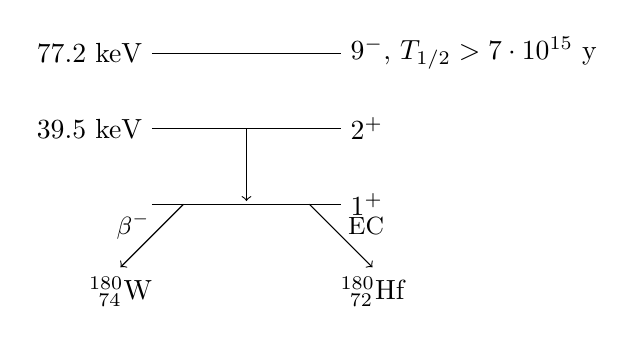
\begin{tikzpicture}[scale=0.8]
\draw (0,0) -- (3,0) node[right]{$1^+$};
\draw (0,1.2) -- (3,1.2) node[right]{$2^+$} node[pos=0,left]{39.5 keV};
\draw (0,2.4) -- (3,2.4) node[right]{$9^-$, $T_{1/2}>7\cdot10^{15}$ y} node[pos=0,left]{77.2 keV};
\draw[->,decorate] (1.5,1.2) -- (1.5,0.05);
\draw[->] (0.5,0) -- (-0.5,-1) node[below]{${}^{180}_{\ 74}$W};
\node at (-0.3,-0.35) {\small $\beta^-$};
\draw[->] (2.5,0) -- (3.5,-1) node[below]{${}^{180}_{\ 72}$Hf};
\node at (3.4,-0.35) {\small EC};
\end{tikzpicture}
\end{center}
Other examples are Tc isotopes.
% TODO: check -- handwritten "Te"/"Tc" isotopes

The electromagnetic reduced probabilities can be expressed in units
\[
[B(E\lambda)]=e^2\,\text{fm}^{2\lambda},\qquad [B(M\lambda)]=\mu_N^2\,\text{fm}^{2\lambda-2},\qquad \mu_N=\frac{e\hbar}{2m}.
\]

\subsection{Single-particle estimates}
It is useful to make a ``single-particle'' estimate for $B(X\lambda)$. With
$\braket{\sigma,\vec r|n\ell jm}=R_{n\ell}(r)\big[Y_\ell\,\chi^{1/2}\big]^j_m$,
\[
\braket{n_f\ell_fj_fm_f|\op{\mathcal M}^E_{\lambda\mu}|n_i\ell_ij_im_i}
=e\int_0^\infty r^{2+\lambda}R_{n_f\ell_f}R_{n_i\ell_i}\,\ud r\;\braket{\ell_fj_fm_f|Y_{\lambda\mu}|\ell_ij_im_i},
\]
\[
\braket{\ell_fj_fm_f|Y_{\lambda\mu}|\ell_ij_im_i}=\sum_{\substack{m_{\ell_i}m_{s_i}\\m_{\ell_f}m_{s_f}}}\big(\ell_im_{\ell_i}\,\tfrac12m_{s_i}\big|j_im_i\big)\big(\ell_fm_{\ell_f}\,\tfrac12m_{s_f}\big|j_fm_f\big)
\]
\[
\times\underbrace{\chi^{1/2\,\dagger}_{m_{s_f}}\chi^{1/2}_{m_{s_i}}}_{\delta_{m_{s_f}m_{s_i}}}
\int Y^*_{\ell_fm_{\ell_f}}Y_{\lambda\mu}Y_{\ell_im_{\ell_i}}\,\ud\Omega .
\]
Using the Wigner--Eckart theorem
\[
\braket{n_f\ell_fj_fm_f|\op{\mathcal M}^E_{\lambda\mu}|n_i\ell_ij_im_i}=\frac{1}{\sqrt{2j_f+1}}\big(j_im_i\,\lambda\mu\big|j_fm_f\big)\braket{n_f\ell_fj_f\|\op{\mathcal M}^E_\lambda\|n_i\ell_ij_i},
\]
\[
B(E\lambda,i\to f)=\frac{\big|\braket{n_f\ell_fj_f\|\op{\mathcal M}^E_\lambda\|n_i\ell_ij_i}\big|^2}{2j_i+1}
=\frac{e^2}{2j_i+1}\Big[\int_0^\infty r^{2+\lambda}R_{n_f\ell_f}R_{n_i\ell_i}\,\ud r\Big]^2\big|\braket{\ell_fj_f\|Y_\lambda\|\ell_ij_i}\big|^2
\]
\[
=\frac{e^2}{4\pi}\Big[\int_0^\infty r^{2+\lambda}R_{n_f\ell_f}R_{n_i\ell_i}\,\ud r\Big]^2 S(\ell_fj_f,\ell_ij_i,\lambda),
\qquad
S(\ell_fj_f,\ell_ij_i,\lambda)=\frac{4\pi}{2j_i+1}\big|\braket{\ell_fj_f\|Y_\lambda\|\ell_ij_i}\big|^2 .
\]
% TODO: check the definition of the geometric factor S (top of handwritten p. 9, w10)

\paragraph{Weisskopf estimate.} We take a constant radial wave function inside the nucleus ($R$ --- nuclear radius)
\[
R_{n\ell}(r)=\begin{cases}C, & r\le R,\\ 0, & r>R,\end{cases}
\qquad
\int_0^\infty\ud r\,|R_{n\ell}|^2r^2=C^2\frac{R^3}{3}\overset{!}{=}1\ \Rightarrow\ C=\sqrt{\frac{3}{R^3}},
\]
and $S\approx1$:
\[
B(E\lambda)_W=\frac{e^2}{4\pi}\,\frac{9}{R^6}\Big[\int_0^Rr^{2+\lambda}\ud r\Big]^2=\frac{9}{4\pi}\,e^2\,\frac{1}{R^6}\Big(\frac{R^{\lambda+3}}{\lambda+3}\Big)^2 .
\]
With $R=r_0A^{1/3}$, $r_0=1.2$~fm,
\[
B(E\lambda)_W=\frac{(1.2)^{2\lambda}}{4\pi}\Big(\frac{3}{\lambda+3}\Big)^2A^{2\lambda/3}\ \big[e^2\,\text{fm}^{2\lambda}\big]\equiv1\ \text{Weisskopf unit (W.u.)}
\]
Similarly one can calculate the estimate for magnetic transitions
\[
B(M\lambda)_W=\frac{10}{\pi}(1.2)^{2\lambda-2}\Big(\frac{3}{\lambda+3}\Big)^2A^{(2\lambda-2)/3}\ \big[\mu_N^2\,\text{fm}^{2\lambda-2}\big]=1\ \text{W.u.}
\]
\underline{Weisskopf units depend on $A$!}

For a pure electric transition of multipolarity $\lambda$
\[
T^E_W(\lambda)=\frac{8\pi c\,\alpha}{e^2}\,\frac{(\hbar\omega)^{2\lambda+1}}{(\hbar c)^{2\lambda+1}}\,\frac{\lambda+1}{\lambda}\,\frac{1}{\big[(2\lambda+1)!!\big]^2}\,B(E\lambda)_W .
\]
Let us compare $T^E_W(\lambda)$ and $T^E_W(\lambda+1)$:
\[
\frac{T^E_W(\lambda+1)}{T^E_W(\lambda)}=\frac{(\hbar\omega)^{2\lambda+3}/(\hbar c)^{2\lambda+3}}{(\hbar\omega)^{2\lambda+1}/(\hbar c)^{2\lambda+1}}\,\frac{\lambda+2}{\lambda+1}\,\frac{\lambda}{\lambda+1}\,\frac{\big[(2\lambda+1)!!\big]^2}{\big[(2\lambda+3)!!\big]^2}\,\frac{B(E\lambda{+}1)_W}{B(E\lambda)_W},
\]
\[
\frac{B(E\lambda{+}1)_W}{B(E\lambda)_W}=\frac{(1.2)^{2\lambda+2}}{(1.2)^{2\lambda}}\Big(\frac{3}{\lambda+4}\Big)^2A^{(2\lambda+2)/3}\Big(\frac{\lambda+3}{3}\Big)^2\frac{1}{A^{2\lambda/3}},
\]
\[
\frac{T^E_W(\lambda+1)}{T^E_W(\lambda)}=\Big(\frac\omega c\Big)^2\frac{\lambda(\lambda+2)}{(\lambda+1)^2}\,\frac{1}{(2\lambda+3)^2}\,
\underbrace{(1.2)^2\,\frac{(\lambda+3)^2}{(\lambda+4)^2}\,A^{2/3}}_{\sim R^2},
\qquad k=\frac\omega c ,
\]
\[
\frac{T^E_W(\lambda+1)}{T^E_W(\lambda)}\sim(kR)^2\ll1 .
\]
The condition $kR\ll1$ means that the wavelength is much larger than the nucleus, $\lambda_\gamma\gg R$:
\[
\frac{E}{\hbar c}R\ll1\quad\Rightarrow\quad E\ll\frac{\hbar c}{R}=\frac{197\ \text{MeV fm}}{7\ \text{fm}}\simeq28\ \text{MeV},
\]
\[
k=\frac\omega c=\frac{2\pi}{\lambda_\gamma},\qquad \lambda_\gamma=\frac{2\pi\hbar c}{\hbar\omega}=\frac{2\pi\cdot197\ \text{MeV fm}}{E_\gamma},
\qquad 1\ \text{MeV}\ \to\ 1238\ \text{fm}.
\]

\paragraph{Note:} $E0$ via emission of a single photon is forbidden, because the spin of the photon is 1. However, e.g.\ a $0^+\to0^+$ transition can occur via internal conversion ($K$, $L$, $M$, \dots\ electrons).

%=====================================================================
\section{Collective states in nuclei (vibrational and rotational degrees of freedom)}
%=====================================================================
In collective models we significantly reduce the number of degrees of freedom by the use of collective coordinates describing special types of excitations. Typical examples are vibrations (of the surface) and collective rotations.

One option for introducing collective coordinates is related to the liquid-drop picture of the nucleus. The distance of the surface from the centre can be parametrized as
\[
R(\vartheta,\varphi,t)=R_0\Big[1+\sum_{\lambda\mu}\alpha^*_{\lambda\mu}(t)\,Y_{\lambda\mu}(\vartheta,\varphi)\Big],
\]
where we introduced the collective variables (coordinates) $\alpha_{\lambda\mu}(t)$.
We require $R\overset{!}{=}R^*$:
\[
\sum_{\lambda\mu}\alpha^*_{\lambda\mu}Y_{\lambda\mu}\overset{!}{=}\sum_{\lambda\mu}\alpha_{\lambda\mu}\underbrace{Y^*_{\lambda\mu}}_{(-1)^\mu Y_{\lambda-\mu}}
\quad\Rightarrow\quad
\alpha^*_{\lambda\mu}=(-1)^\mu\,\alpha_{\lambda-\mu}.
\]

\subsection{Transformation properties of \texorpdfstring{$\alpha_{\lambda\mu}$}{alpha}}
Let us assume 2 coordinate frames: $x,y,z$ $\to$ laboratory, $x',y',z'$ $\to$ rotated.
\begin{center}
\begin{tikzpicture}[scale=1.0]
\draw[->,thick] (0,0) -- (0,2.2) node[above]{$z$};
\draw[->,thick] (0,0) -- (2.5,0) node[right]{$y$};
\draw[->,thick] (0,0) -- (-1.3,-1.3) node[below left]{$x$};
\begin{scope}[rotate=-30]
\draw[->,thick,red!70!black] (0,0) -- (0,2.0) node[above]{$z'$};
\draw[->,thick,red!70!black] (0,0) -- (1.0,-1.6) node[below]{$y'$};
\draw[->,thick,red!70!black] (0,0) -- (-1.8,0.4) node[left]{$x'$};
\end{scope}
\end{tikzpicture}
\end{center}
In the rotated frame $x',y',z'$
\[
R(\vartheta',\varphi',t)=R_0\Big[1+\sum_{\lambda\mu}\alpha'^*_{\lambda\mu}\,Y_{\lambda\mu}(\vartheta',\varphi')\Big],
\]
where $\vartheta',\varphi'$ are the angles referred to the rotated system $x',y',z'$. The spherical harmonics are transformed as
\[
Y_{\lambda\mu}(\vartheta',\varphi')=\sum_\nu D^\lambda_{\nu\mu}(\alpha,\beta,\gamma)\,Y_{\lambda\nu}(\vartheta,\varphi),
\]
with the Euler angles $(\alpha,\beta,\gamma)$ corresponding to the rotation $x,y,z\to x',y',z'$.
Invariance of $R$ under rotations, $R(\vartheta',\varphi',t)=R(\vartheta,\varphi,t)$, gives
\[
\sum_{\lambda\mu}\alpha'^*_{\lambda\mu}Y_{\lambda\mu}(\vartheta',\varphi')=\sum_{\lambda\mu}\alpha^*_{\lambda\mu}Y_{\lambda\mu}(\vartheta,\varphi),
\]
\[
\sum_{\lambda\mu}\sum_\nu\alpha'^*_{\lambda\mu}D^\lambda_{\nu\mu}(\alpha,\beta,\gamma)\,Y_{\lambda\nu}(\vartheta,\varphi)=\sum_{\lambda\mu}\alpha^*_{\lambda\mu}Y_{\lambda\mu}(\vartheta,\varphi),
\]
and exchanging $\mu\leftrightarrow\nu$
\[
\sum_{\lambda\mu\nu}\alpha'^*_{\lambda\nu}D^\lambda_{\mu\nu}(\alpha,\beta,\gamma)\,Y_{\lambda\mu}(\vartheta,\varphi)=\sum_{\lambda\mu}\alpha^*_{\lambda\mu}Y_{\lambda\mu}(\vartheta,\varphi)
\quad\Rightarrow\quad
\sum_\nu\alpha'^*_{\lambda\nu}D^\lambda_{\mu\nu}=\alpha^*_{\lambda\mu}.
\]
Using the unitarity $\sum_\mu D^\lambda_{\mu\nu}(\alpha,\beta,\gamma)D^{\lambda*}_{\mu\sigma}(\alpha,\beta,\gamma)=\delta_{\nu\sigma}$,
\[
\sum_{\mu\nu}\alpha'^*_{\lambda\nu}\underbrace{D^{\lambda*}_{\mu\sigma}(\alpha,\beta,\gamma)D^\lambda_{\mu\nu}(\alpha,\beta,\gamma)}_{\delta_{\nu\sigma}}=\sum_\mu D^{\lambda*}_{\mu\sigma}(\alpha,\beta,\gamma)\,\alpha^*_{\lambda\mu}
\quad\Rightarrow\quad
\alpha'^*_{\lambda\sigma}=\sum_\mu D^{\lambda*}_{\mu\sigma}\alpha^*_{\lambda\mu}
\]
\[
\Rightarrow\quad \alpha'_{\lambda\mu}=\sum_\nu D^\lambda_{\nu\mu}\,\alpha_{\lambda\nu}
\qquad(\text{like } Y_{\lambda\mu}),
\]
i.e.\ $\alpha_{\lambda\mu}$ are transformed as \textbf{spherical tensors}.

Parity transformation $\op P$: $r\to r$, $\vartheta\to\pi-\vartheta$, $\varphi\to\varphi+\pi$,
\[
\op P^{-1}Y_{\lambda\mu}\op P=(-1)^\lambda Y_{\lambda\mu}.
\]
\[
\Rightarrow\quad \alpha'_{\lambda\mu}=\op P\alpha_{\lambda\mu}\op P^{-1}=(-1)^\lambda\alpha_{\lambda\mu}.
\]

\subsection{Volume conservation and the lowest modes}
For an incompressible liquid drop described by the function $R(\vartheta,\varphi)\equiv R(\Omega)$, the volume is
\[
V=\int\ud\Omega\int_0^{R(\Omega)}r^2\ud r=\frac13R_0^3\int\ud\Omega\Big(1+\sum_{\lambda\mu}\alpha^*_{\lambda\mu}Y_{\lambda\mu}\Big)^3
\]
\[
\approx\frac{R_0^3}{3}\int\ud\Omega\Big(1+3\sum_{\lambda\mu}\alpha^*_{\lambda\mu}Y_{\lambda\mu}
\]
\[
+3\sum_{\substack{\lambda\mu\\\lambda'\mu'}}\alpha^*_{\lambda\mu}\alpha^*_{\lambda'\mu'}Y_{\lambda\mu}\underbrace{Y_{\lambda'\mu'}}_{(-1)^{\mu'}Y^*_{\lambda'-\mu'}}+\dots\Big).
\]
Using $1=\sqrt{4\pi}\,Y^*_{00}$ and $\int\ud\Omega\,Y^*_{\lambda\mu}Y_{\lambda'\mu'}=\delta_{\lambda\lambda'}\delta_{\mu\mu'}$,
\[
V=\frac{R_0^3}{3}\Big(4\pi+3\sqrt{4\pi}\,\alpha_{00}+3\sum_{\lambda\mu}\alpha^*_{\lambda\mu}\underbrace{(-1)^\mu\alpha^*_{\lambda-\mu}}_{\alpha_{\lambda\mu}}\Big)
=\frac{R_0^3}{3}\Big(4\pi+3\sqrt{4\pi}\,\alpha_{00}+3\sum_{\lambda\mu}|\alpha_{\lambda\mu}|^2\Big)\overset{!}{=}\frac43\pi R_0^3
\]
\[
\Rightarrow\quad \alpha_{00}=-\frac{1}{\sqrt{4\pi}}\sum_{\lambda\mu}|\alpha_{\lambda\mu}|^2 .
\]
The lowest modes:
\begin{itemize}
\item $\lambda=0$ --- monopole (compressional, ``breathing'' mode). In nuclei it exists at relatively high energies (40--50~MeV) due to the low compressibility of nuclear matter.
\item $\lambda=1$ --- dipole. The centre of mass is
\[
\vec R=\frac{\int\ud^3r\,\vec r\rho(\vec r)}{\int\ud^3r\,\rho(\vec r)},
\qquad\text{if }\rho=\text{const.:}\quad \vec R=\frac1V\int\ud^3r\,\vec r .
\]
In spherical components $r_\mu=\sqrt{4\pi/3}\,r\,Y_{1\mu}$ ($r_0=z$, $r_{\pm1}=\mp\frac{1}{\sqrt2}(x\pm iy)$):
\[
R_\mu=\frac1V\int\ud^3r\,r_\mu=\frac1V\sqrt{\frac{4\pi}{3}}\int\ud\Omega\int_0^{R(\Omega)}\ud r\,r^3\,Y_{1\mu}(\Omega)
\]
\[
=\sqrt{\frac{3}{4\pi}}\,\frac{1}{R_0^3}\,\frac{R_0^4}{4}\int\ud\Omega\Big(1+4\sum_{\lambda\nu}\alpha_{\lambda\nu}Y^*_{\lambda\nu}\Big)Y_{1\mu}
\]
\[
\Rightarrow\quad R_\mu=\sqrt{\frac{3}{4\pi}}\,R_0\,\alpha_{1\mu},
\]
i.e.\ for small $\alpha$ the dipole mode corresponds to a translation of the CM.
\item $\lambda=2$ --- quadrupole vibrations ($2^+$ low-lying states).
\item $\lambda=3$ --- octupole vibrations ($3^-$ low-lying states).
\end{itemize}
\begin{center}
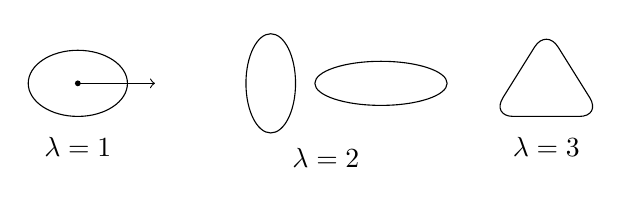
\begin{tikzpicture}[scale=0.7]
\draw (0,0) ellipse (0.9 and 0.6); \fill (0,0) circle (1.5pt); \draw[->] (0,0) -- (1.4,0);
\node[below] at (0,-0.8) {$\lambda=1$};
\draw (3.5,0) ellipse (0.45 and 0.9); \draw (5.5,0) ellipse (1.2 and 0.4);
\node[below] at (4.5,-1.0) {$\lambda=2$};
\draw[rounded corners=8pt] (7.5,-0.6) -- (8.5,1.0) -- (9.5,-0.6) -- cycle;
\node[below] at (8.5,-0.8) {$\lambda=3$};
\end{tikzpicture}
\end{center}
In nuclei, the quadrupole deformation plays a significant role and will be discussed in more detail.

\subsection{Quadrupole deformation}
For $\lambda=2$
\[
R(\vartheta,\varphi)=R_0\Big(1+\sum_{\mu=0,\pm1,\pm2}\alpha^*_{2\mu}Y_{2\mu}(\vartheta,\varphi)\Big)
\]
(translations $\alpha_{1\mu}$ are not intrinsic excitations and $\alpha_{00}\sim|\alpha_{2\mu}|^2$ is quadratic $\to$ for small $\alpha$ it can be neglected). With $\alpha^*_{2\mu}=(-1)^\mu\alpha_{2-\mu}$, the complex $\alpha_{2\mu}$ represent 5 independent variables.

Let us explore the relation to Cartesian coordinates. Insertion of ($x=r\sin\vartheta\cos\varphi$, $y=r\sin\vartheta\sin\varphi$, $z=r\cos\vartheta$)
\[
Y_{20}=\sqrt{\frac{5}{16\pi}}\,\frac{1}{r^2}\big(2z^2-x^2-y^2\big),\qquad
Y_{2\pm1}=\mp\sqrt{\frac{15}{8\pi}}\,\frac{1}{r^2}\big(xz\pm izy\big),
\]
\[
Y_{2\pm2}=\sqrt{\frac{15}{32\pi}}\,\frac{1}{r^2}\big(x^2-y^2\pm2ixy\big)
\]
into $R(\vartheta,\varphi)$ gives
\[
R=R_0\Big(1+a_{xx}\frac{x^2}{r^2}+a_{yy}\frac{y^2}{r^2}+a_{zz}\frac{z^2}{r^2}+2a_{xy}\frac{xy}{r^2}+2a_{yz}\frac{yz}{r^2}+2a_{xz}\frac{xz}{r^2}\Big).
\]
By comparison we get
\[
\alpha_{2\pm2}=\sqrt{\frac{8\pi}{15}}\,\frac12\big(a_{xx}-a_{yy}\pm2ia_{xy}\big),\qquad
\alpha_{2\pm1}=\mp\sqrt{\frac{8\pi}{15}}\big(a_{xz}\pm ia_{yz}\big),
\]
\[
\alpha_{20}=\sqrt{\frac{8\pi}{15}}\,\frac{1}{\sqrt6}\big(2a_{zz}-a_{xx}-a_{yy}\big).
\]
$a_{xx},a_{yy},a_{zz},a_{xy},a_{yz},a_{xz}$ $\to$ 6 parameters, but $\alpha_{2\mu}$ --- only 5 parameters: $a_{xx}+a_{yy}+a_{zz}=0$.
Indeed, consider the integrals
\[
\int\frac{x^2}{r^2}\ud\Omega=\int\frac{y^2}{r^2}\ud\Omega=\int\frac{z^2}{r^2}\ud\Omega\equiv A,
\qquad
\int\frac{xy}{r^2}\ud\Omega=\int\frac{yz}{r^2}\ud\Omega=\int\frac{xz}{r^2}\ud\Omega=0 .
\]
Then
\[
\int R\,\ud\Omega=4\pi R_0+R_0A\big(a_{xx}+a_{yy}+a_{zz}\big)
\overset{!}{=}\int R_0\Big(1+\sum_\mu\alpha^*_{2\mu}Y_{2\mu}\Big)\ud\Omega=4\pi R_0 ,
\]
because $\int Y_{2\mu}\ud\Omega=0$ $\Rightarrow$ $A(a_{xx}+a_{yy}+a_{zz})=0$.

Further, we can rotate the frame $x,y,z\xrightarrow{\ \mathcal R\ }x',y',z'$ such that $a'_{xy}=a'_{yz}=a'_{xz}=0$ (principal axes):
\[
\Rightarrow\quad \alpha'_{2\pm1}=0,\qquad
\alpha'_{2\pm2}=\frac12\sqrt{\frac{8\pi}{15}}\big(a'_{xx}-a'_{yy}\big)\equiv a_2,\qquad
\alpha'_{20}=\sqrt{\frac{8\pi}{15}}\,\frac{1}{\sqrt6}\big(2a'_{zz}-a'_{xx}-a'_{yy}\big)\equiv a_0 .
\]
$\Rightarrow$ instead of 5 parameters $\alpha_{2\mu}$ we can use 2 parameters for the deformation $(a_2,a_0)$ $+$ 3 angles (e.g.\ Euler) describing the rotation $(x,y,z)\to(x',y',z')$ to the \textbf{intrinsic frame}.

In nuclear physics, further, we parametrize $a_0,a_2$ as follows:
\[
a_0=\beta\cos\gamma,\qquad a_2=\frac{1}{\sqrt2}\,\beta\sin\gamma ,
\]
$\beta,\gamma$ are the so-called \textbf{Bohr deformation parameters}.

We can construct scalars from $\alpha_{2\mu}$. Using $\big(jm\,j\,{-m}\big|00\big)=(-1)^{j-m}\frac{1}{\sqrt{2j+1}}$,
\[
\big[\alpha_2\times\alpha_2\big]^0_0=\sum_\mu\big(2\mu\,2\,{-\mu}\big|00\big)\alpha_{2\mu}\alpha_{2-\mu}
=\sum_\mu(-1)^{\mu}\frac{1}{\sqrt5}\,\alpha_{2\mu}\alpha_{2-\mu}
=\frac{1}{\sqrt5}\sum_\mu\alpha_{2\mu}\alpha^*_{2\mu}=\frac{1}{\sqrt5}\sum_\mu|\alpha_{2\mu}|^2
\]
\[
=\big[\alpha'_2\times\alpha'_2\big]^0=\frac{1}{\sqrt5}\sum_\mu|\alpha'_{2\mu}|^2=\frac{1}{\sqrt5}\big(2a_2^2+a_0^2\big)=\frac{1}{\sqrt5}\,\beta^2
\quad\Rightarrow\quad \beta^2=\sum_\mu|\alpha_{2\mu}|^2\ \text{is invariant}.
\]
Another example:
\[
\Big[\big[\alpha_2\times\alpha_2\big]^2\times\alpha_2\Big]^0_0=\Big[\big[\alpha'_2\times\alpha'_2\big]^2\times\alpha'_2\Big]^0_0
=\sum_\mu\underbrace{\big(2\mu\,2\,{-\mu}\big|00\big)}_{(-1)^\mu/\sqrt5}\big[\alpha'_2\times\alpha'_2\big]^2_\mu\,\alpha'_{2-\mu}
\]
\[
=\frac{1}{\sqrt5}\sum_\mu(-1)^\mu\sum_{\nu\nu'}\big(2\nu\,2\nu'\big|2\mu\big)\alpha'_{2\nu}\alpha'_{2\nu'}\alpha'_{2-\mu}
\]
\[
=\frac{1}{\sqrt5}\Big(\alpha'_{20}\sum_\nu\big(2\nu\,2\,{-\nu}\big|20\big)\alpha'_{2\nu}\alpha'_{2-\nu}
+\alpha'_{2-2}\sum_{\nu\nu'}\big(2\nu\,2\nu'\big|22\big)\alpha'_{2\nu}\alpha'_{2\nu'}
+\alpha'_{22}\sum_{\nu\nu'}\big(2\nu\,2\nu'\big|2\,{-2}\big)\alpha'_{2\nu}\alpha'_{2\nu'}\Big)
\]
(only $\alpha'_{20}$ and $\alpha'_{2\pm2}$ are nonzero in the intrinsic frame)
\[
=\frac{1}{\sqrt5}\Big[\alpha'_{20}\Big\{\underbrace{\big(22\,2{-}2\big|20\big)}_{\sqrt{2/7}}\alpha'_{22}\alpha'_{2-2}+\underbrace{\big(2{-}2\,22\big|20\big)}_{\sqrt{2/7}}\alpha'_{2-2}\alpha'_{22}+\underbrace{\big(20\,20\big|20\big)}_{-\sqrt{2/7}}\alpha'_{20}\alpha'_{20}\Big\}
\]
\[
+\alpha'_{2-2}\Big\{\underbrace{\big(20\,22\big|22\big)}_{\sqrt{2/7}}\alpha'_{20}\alpha'_{22}+\underbrace{\big(22\,20\big|22\big)}_{\sqrt{2/7}}\alpha'_{22}\alpha'_{20}\Big\}
\]
\[
+\alpha'_{22}\Big\{\underbrace{\big(20\,2{-}2\big|2{-}2\big)}_{\sqrt{2/7}}\alpha'_{20}\alpha'_{2-2}+\underbrace{\big(2{-}2\,20\big|2{-}2\big)}_{\sqrt{2/7}}\alpha'_{2-2}\alpha'_{20}\Big\}\Big]
\]
\[
=\sqrt{\frac{2}{35}}\Big[\beta\cos\gamma\Big(2\cdot\frac12\beta^2\sin^2\gamma-\beta^2\cos^2\gamma\Big)
+\frac{1}{\sqrt2}\beta\sin\gamma\cdot4\beta\cos\gamma\cdot\frac{1}{\sqrt2}\beta\sin\gamma\Big]
\]
\[
=\sqrt{\frac{2}{35}}\,\beta^3\Big(\cos\gamma\big(-\cos2\gamma\big)+\sin2\gamma\,\sin\gamma\Big)
=-\sqrt{\frac{2}{35}}\,\beta^3\cos3\gamma ,
\]
where we used $\sin2x=2\sin x\cos x$, $\cos2x=\cos^2x-\sin^2x$.
$\Rightarrow$ $\beta^3\cos3\gamma$ is invariant.

\subsection{Shapes in the parametric space \texorpdfstring{$\beta,\gamma$}{beta, gamma}}
The half-axes of the deformed nucleus in the intrinsic frame are
\[
R_1=R(\vartheta'{=}\tfrac\pi2,\varphi'{=}0),\qquad
R_2=R(\vartheta'{=}\tfrac\pi2,\varphi'{=}\tfrac\pi2),\qquad
R_3=R(\vartheta'{=}0,\varphi'),
\]
\begin{center}
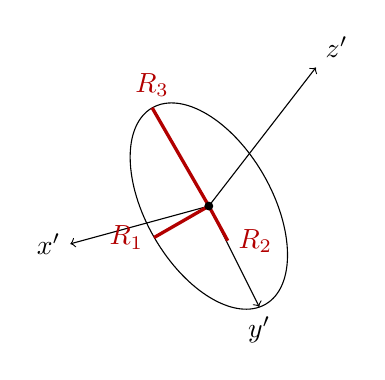
\begin{tikzpicture}[scale=0.8]
\draw[rotate=30] (0,0) ellipse (1.0 and 1.8);
\draw[->] (0,0) -- (1.7,2.2) node[above right]{$z'$};
\draw[->] (0,0) -- (-2.2,-0.6) node[left]{$x'$};
\draw[->] (0,0) -- (0.8,-1.6) node[below]{$y'$};
\draw[very thick,red!70!black] (0,0) -- (-0.9,1.56) node[above]{$R_3$};
\draw[very thick,red!70!black] (0,0) -- (-0.87,-0.5) node[left]{$R_1$};
\draw[very thick,red!70!black] (0,0) -- (0.3,-0.55) node[right]{$R_2$};
\fill (0,0) circle (2pt);
\end{tikzpicture}
\end{center}
\[
R_i=R_0\big(1+\delta R_i\big),\qquad
\delta R_i\equiv\frac{R_i-R_0}{R_0}=\sqrt{\frac{5}{4\pi}}\,\beta\cos\Big(\gamma-\frac{2\pi}{3}i\Big),\qquad i=1,2,3 .
\]
Indeed,
\[
R=R_0\big[1+a_0Y_{20}+a_2(Y_{22}+Y_{2-2})\big]
=R_0\Big[1+a_0\sqrt{\frac{5}{16\pi}}\big(2n_z^2-n_x^2-n_y^2\big)+a_2\sqrt{\frac{15}{32\pi}}\big(n_x^2-n_y^2\big)\Big]
\]
\[
=R_0\Big[1+\beta\cos\gamma\sqrt{\frac{5}{16\pi}}\big(3\cos^2\vartheta-1\big)+\frac{1}{\sqrt2}\beta\sin\gamma\sqrt{\frac{15}{32\pi}}\,2\sin^2\vartheta\cos2\varphi\Big],
\]
where $\vec n=\vec r/r$. Then
\[
R_1=R(\vartheta{=}\tfrac\pi2,\varphi{=}0)=R_0\Big[1-\sqrt{\frac{5}{16\pi}}\beta\cos\gamma+\sqrt{\frac{15}{16\pi}}\beta\sin\gamma\Big]
\]
\[
=R_0\Big[1+\sqrt{\frac{5}{4\pi}}\beta\Big(\underbrace{-\tfrac12}_{\cos\frac{2\pi}{3}}\cos\gamma+\underbrace{\tfrac{\sqrt3}{2}}_{\sin\frac{2\pi}{3}}\sin\gamma\Big)\Big]
=R_0\Big[1+\sqrt{\frac{5}{4\pi}}\beta\cos\Big(\gamma-\frac{2\pi}{3}\Big)\Big],
\]
\[
R_2=R(\vartheta{=}\tfrac\pi2,\varphi{=}\tfrac\pi2)=R_0\Big[1-\sqrt{\frac{5}{16\pi}}\beta\cos\gamma-\sqrt{\frac{15}{16\pi}}\beta\sin\gamma\Big]
\]
\[
=R_0\Big[1+\sqrt{\frac{5}{4\pi}}\beta\Big(\underbrace{-\tfrac12}_{\cos\frac{4\pi}{3}}\cos\gamma\underbrace{-\tfrac{\sqrt3}{2}}_{\sin\frac{4\pi}{3}}\sin\gamma\Big)\Big]
=R_0\Big[1+\sqrt{\frac{5}{4\pi}}\beta\cos\Big(\gamma-\frac{4\pi}{3}\Big)\Big],
\]
\[
R_3=R(\vartheta{=}0,\varphi)=R_0\Big[1+\sqrt{\frac{5}{16\pi}}\beta\cos\gamma\cdot2\Big]=R_0\Big[1+\sqrt{\frac{5}{4\pi}}\beta\cos\Big(\gamma-\frac{6\pi}{3}\Big)\Big].
\]
For $\beta>0$: $\gamma=0$ --- prolate (axially symmetric), $\gamma=\pi/3$ --- oblate (axially symmetric), $\gamma\neq0,\pi/3$ --- triaxial.
\begin{center}
\begin{tikzpicture}[scale=1.0]
\draw[->] (0,0) -- (4,0) node[right]{$\beta$};
\draw[->] (0,0) -- (60:4) ;
\draw (1,0) arc (0:60:1); \node at (30:1.3) {$\pi/3$};
\draw (4.6,-0.1) ellipse (0.3 and 0.55); \node[right] at (5.0,-0.1) {prolate ($\gamma=0$)};
\draw (60:4.5) ellipse (0.55 and 0.2); \node[right] at ($(60:4.5)+(0.6,0)$) {oblate ($\gamma=\pi/3$)};
\node at (2.6,1.0) {triaxial};
\end{tikzpicture}
\end{center}
To describe a general quadrupole deformation, we can parametrize it in terms of $\alpha_{2\mu}$, or $(\beta,\gamma)$ --- deformation parameters $+$ $(\vartheta_1,\vartheta_2,\vartheta_3)$ --- Euler angles.

\paragraph{Note:} The definition of the variables $\alpha_{2\mu}$ can be generalized in the sense that $\alpha_{2\mu}$ can describe not only the parametrisation of the surface, but e.g.\ surfaces of constant densities, or components of the quadrupole tensor
\[
\alpha_{2\mu}=\sum_{i=1}^Ar_i^2\,Y_{2\mu}(\vartheta_i,\varphi_i)\qquad\text{or}\qquad
\alpha_{2\mu}=\int r^2\,Y_{2\mu}\,\rho(\vec r)\,\ud^3r .
\]

%=====================================================================
\section{Surface vibrations of spherical nuclei}
%=====================================================================
Let us assume a classical charged liquid-drop picture. The total energy is given by the kinetic term, the Coulomb energy ($E_C$) and the surface energy ($E_S$),
\[
E=T+E_C+E_S .
\]
The drop is parametrized by the collective variables $\alpha_{\lambda\mu}$:
\[
R(\Omega)=R_0\Big(1+\sum_{\lambda\mu}\alpha^*_{\lambda\mu}Y_{\lambda\mu}(\Omega)\Big).
\]
The kinetic energy can be calculated as
\[
T=\int\ud^3r\,\frac12\rho_m(\vec r)\,\vec v^{\,2}(\vec r,t),
\]
where $\rho_m$ is the mass density and $\vec v$ is the velocity field. For constant density $\rho_m$ and a non-vortical (irrotational) field ($\vec\nabla\times\vec v=0$), the kinetic energy can be expanded in terms of $\dot\alpha$:
\[
T=\int\ud\Omega\int_0^{R(\Omega)}r^2\,\frac12\rho_m\vec v^{\,2}\,\ud r\approx\frac12\rho_mR_0^5\sum_{\lambda\mu}\frac1\lambda\,|\dot\alpha_{\lambda\mu}|^2,
\qquad \dot\alpha\equiv\frac{\ud\alpha}{\ud t}.
\]
The contribution to the potential energy from the Coulomb interaction is
\[
E_C=\frac12\int\ud^3r\int\ud^3r'\,\frac{\rho_c(\vec r)\rho_c(\vec r\,')}{|\vec r-\vec r\,'|}\cdot\frac{1}{4\pi\varepsilon_0}
\]
\[
=\frac12\int\ud\Omega\int\ud\Omega'\int_0^{R(\Omega)}r^2\ud r\int_0^{R(\Omega')}r'^2\ud r'\,\frac{\rho_c(\vec r)\rho_c(\vec r\,')}{|\vec r-\vec r\,'|}\cdot\frac{1}{4\pi\varepsilon_0},
\]
where $\rho_c$ is the charge density. We can assume $\rho_c=\text{const}$,
\[
\rho_c=\frac{Ze}{\frac43\pi R_0^3},\qquad R_0=r_0A^{1/3}.
\]
One can show that
\[
E_C=E_C^{(0)}\Big(1-\frac{5}{4\pi}\sum_{\lambda\mu}\frac{\lambda-1}{2\lambda+1}|\alpha_{\lambda\mu}|^2+\dots\Big),
\]
where
\[
E_C^{(0)}=\frac35\,\frac{Z^2e^2}{4\pi\varepsilon_0R_0}
\]
is the Coulomb energy of a uniformly charged sphere (total charge $Ze$) with radius $R_0$.
The surface energy, under the assumption of a constant surface tension $\sigma$, is
\[
E_S=\sigma\int\ud S=E_S^{(0)}\Big[1+\frac{1}{8\pi}\sum_{\lambda\mu}(\lambda-1)(\lambda+2)|\alpha_{\lambda\mu}|^2+\dots\Big],
\]
where
\[
E_S^{(0)}=4\pi R_0^2\sigma
\]
is the surface energy of a sphere with radius $R_0$. (Derivations of $T$, $E_S$, $E_C$ can be found in the literature, e.g.\ V.~Zelevinsky, A.~Volya: \emph{Physics of Atomic Nuclei}.)

The classical Hamiltonian therefore can be written as (if we neglect higher powers of $\dot\alpha$, $\alpha$)
\[
H=T+V=\frac12\sum_{\lambda\mu}B_\lambda|\dot\alpha_{\lambda\mu}|^2+\frac12\sum_{\lambda\mu}C_\lambda|\alpha_{\lambda\mu}|^2+\big(E_S^{(0)}+E_C^{(0)}\big)+\dots,
\]
where
\[
B_\lambda=\rho_m\frac{R_0^5}{\lambda}\equiv B_\lambda^{\rm LD},
\]
\[
C_\lambda=2(\lambda-1)\Big[(\lambda+2)\frac{1}{8\pi}E_S^{(0)}-\frac{5}{4\pi}\,\frac{1}{2\lambda+1}\,E_C^{(0)}\Big]
\]
\[
=(\lambda-1)\Big[(\lambda+2)R_0^2\sigma-\frac{3}{2\pi}\,\frac{1}{2\lambda+1}\,\frac{Z^2e'^2}{R_0}\Big]\equiv C_\lambda^{\rm LD},
\qquad e'^2=\frac{e^2}{4\pi\varepsilon_0},
\]
are the liquid-drop (LD) estimates of the ``mass'' ($B_\lambda$) and stiffness ($C_\lambda$) parameters.
The frequency of each mode $\lambda$ is given by
\[
\omega_\lambda=\sqrt{\frac{C_\lambda}{B_\lambda}} .
\]

The surface tension can be extracted from the Bethe--Weizs\"acker (BW) formula:
\[
E_S^{(0)}=4\pi R_0^2\sigma\overset{!}{=}a_SA^{2/3},\qquad R_0=r_0A^{1/3},\ r_0\simeq1.2\ \text{fm},
\qquad
\sigma=\frac{a_SA^{2/3}}{4\pi r_0^2A^{2/3}}=\frac{a_S}{4\pi r_0^2}.
\]
From the BW fit we know the value $a_S=18$~MeV. For $\lambda=2$
\[
C_2^{\rm LD}=\Big[4R_0^2\sigma-\frac{3}{2\pi}\,\frac15\,\frac{Z^2e'^2}{R_0}\Big].
\]
An interesting point corresponds to $C_\lambda^{\rm LD}=0$
\[
\Longleftrightarrow\quad(\lambda+2)E_S^{(0)}=\frac{10}{2\lambda+1}E_C^{(0)},
\]
which corresponds to an \textbf{instability of the drop}. For $\lambda=2$
\[
2E_S^{(0)}=E_C^{(0)}\quad\Longleftrightarrow\quad 2a_SA^{2/3}=\frac35\,\frac{Z^2e'^2}{r_0A^{1/3}} .
\]
We can define the so-called \textbf{fissility parameter}
\[
x\equiv\frac{Z^2}{A}=\frac{10}{3}\,\frac{a_Sr_0}{e'^2}\approx50
\qquad(\text{depending on the value of }a_S),
\qquad e'^2=\alpha\hbar c\approx1.44\ \text{MeV fm}.
\]
It is interesting to evaluate $Z^2/A$ for some nuclei:
\[
\frac{Z^2}{A}\big({}^{238}\text{U}\big)\approx35.6,\qquad \frac{Z^2}{A}\big({}^{244}\text{Cf}\big)\approx39.4 .
\]

\subsection{Quantization of surface vibrations}
We can rewrite the energy in terms of conjugated momenta. One can define the classical Lagrangian
\[
L=\frac12\sum_{\lambda\mu}B_\lambda|\dot\alpha_{\lambda\mu}|^2-\frac12\sum_{\lambda\mu}C_\lambda|\alpha_{\lambda\mu}|^2 .
\]
The momenta are given by
\[
\pi_{\lambda\mu}=\frac{\partial L}{\partial\dot\alpha_{\lambda\mu}}=B_\lambda\,\dot\alpha^*_{\lambda\mu}.
\]
The corresponding Hamiltonian is
\[
H=\frac12\sum_{\lambda\mu}\frac{1}{B_\lambda}|\pi_{\lambda\mu}|^2+\frac12\sum_{\lambda\mu}C_\lambda|\alpha_{\lambda\mu}|^2 ,
\]
and the Hamilton equations are then
\[
\dot\alpha_{\lambda\mu}=\frac{\partial H}{\partial\pi_{\lambda\mu}}=\frac{1}{B_\lambda}\pi^*_{\lambda\mu},\qquad
\dot\pi_{\lambda\mu}=-\frac{\partial H}{\partial\alpha_{\lambda\mu}}=-C_\lambda\,\alpha^*_{\lambda\mu}.
\]
The Hamiltonian can be quantized: $\alpha,\pi\to\op\alpha,\op\pi$,
\[
\op\alpha^\dagger_{\lambda\mu}=(-1)^\mu\op\alpha_{\lambda-\mu},\qquad \op\pi^\dagger_{\lambda\mu}=(-1)^\mu\op\pi_{\lambda-\mu},
\]
with the operators $\op\alpha$, $\op\pi$ satisfying the commutation relations
\[
\big[\op\alpha_{\lambda\mu},\op\alpha^\dagger_{\lambda'\mu'}\big]=0,\qquad
\big[\op\pi_{\lambda\mu},\op\pi^\dagger_{\lambda'\mu'}\big]=0,\qquad
\big[\op\alpha_{\lambda\mu},\op\pi_{\lambda'\mu'}\big]=i\hbar\,\delta_{\lambda\lambda'}\delta_{\mu\mu'}
\quad\Longleftrightarrow\quad \op\pi_{\lambda\mu}=-i\hbar\frac{\partial}{\partial\alpha_{\lambda\mu}},
\]
\[
\op H=\frac12\sum_{\lambda\mu}\frac{1}{B_\lambda}\,\op\pi_{\lambda\mu}\underbrace{(-1)^\mu\op\pi_{\lambda-\mu}}_{\op\pi^\dagger_{\lambda\mu}}
+\frac12\sum_{\lambda\mu}C_\lambda\,\op\alpha_{\lambda\mu}\underbrace{(-1)^\mu\op\alpha_{\lambda-\mu}}_{\op\alpha^\dagger_{\lambda\mu}} .
\]
Let us define the creation and annihilation \textbf{phonon} operators
\[
\op\beta^\dagger_{\lambda\mu}=\sqrt{\frac{B_\lambda\omega_\lambda}{2\hbar}}\,\op\alpha_{\lambda\mu}-i\sqrt{\frac{1}{2B_\lambda\hbar\omega_\lambda}}\,\op\pi^\dagger_{\lambda\mu},
\qquad
\op\beta_{\lambda\mu}=\sqrt{\frac{B_\lambda\omega_\lambda}{2\hbar}}\,\op\alpha^\dagger_{\lambda\mu}+i\sqrt{\frac{1}{2B_\lambda\hbar\omega_\lambda}}\,\op\pi_{\lambda\mu},
\qquad \omega_\lambda=\sqrt{\frac{C_\lambda}{B_\lambda}} .
\]
Then $[\op\beta_{\lambda\mu},\op\beta_{\lambda'\mu'}]=0$ and
\[
\big[\op\beta_{\lambda\mu},\op\beta^\dagger_{\lambda'\mu'}\big]
=\sqrt{\frac{B_\lambda\omega_\lambda}{2\hbar}}(-i)\sqrt{\frac{1}{2B_{\lambda'}\hbar\omega_{\lambda'}}}\underbrace{\big[\op\alpha^\dagger_{\lambda\mu},\op\pi^\dagger_{\lambda'\mu'}\big]}_{i\hbar\delta_{\lambda\lambda'}\delta_{\mu\mu'}}
+i\sqrt{\frac{1}{2B_\lambda\hbar\omega_\lambda}}\sqrt{\frac{B_{\lambda'}\omega_{\lambda'}}{2\hbar}}\underbrace{\big[\op\pi_{\lambda\mu},\op\alpha_{\lambda'\mu'}\big]}_{-i\hbar\delta_{\lambda\lambda'}\delta_{\mu\mu'}}
=\delta_{\lambda\lambda'}\delta_{\mu\mu'}
\]
$\Rightarrow$ bosonic commutation relations. Inversely,
\[
\op\alpha_{\lambda\mu}=\frac12\sqrt{\frac{2\hbar}{B_\lambda\omega_\lambda}}\Big(\op\beta^\dagger_{\lambda\mu}+(-1)^\mu\op\beta_{\lambda-\mu}\Big),
\qquad
\op\pi_{\lambda\mu}=\frac{1}{2i}\sqrt{2B_\lambda\hbar\omega_\lambda}\Big(\op\beta_{\lambda\mu}-(-1)^\mu\op\beta^\dagger_{\lambda-\mu}\Big),
\]
and, using $C_\lambda/B_\lambda=\omega_\lambda^2$,
\[
\op H=\frac12\sum_{\lambda\mu}\frac{1}{B_\lambda}\,\frac14\,2B_\lambda\hbar\omega_\lambda\Big(\op\beta_{\lambda\mu}-(-1)^\mu\op\beta^\dagger_{\lambda-\mu}\Big)\Big(\op\beta^\dagger_{\lambda\mu}-(-1)^\mu\op\beta_{\lambda-\mu}\Big)
\]
\[
+\frac12\sum_{\lambda\mu}C_\lambda\,\frac14\,\frac{2\hbar}{B_\lambda\omega_\lambda}\Big(\op\beta^\dagger_{\lambda\mu}+(-1)^\mu\op\beta_{\lambda-\mu}\Big)\Big(\op\beta_{\lambda\mu}+(-1)^\mu\op\beta^\dagger_{\lambda-\mu}\Big)
\]
\[
=\sum_{\lambda\mu}\frac12\hbar\omega_\lambda\Big(\underbrace{\op\beta_{\lambda\mu}\op\beta^\dagger_{\lambda\mu}}_{1+\op\beta^\dagger_{\lambda\mu}\op\beta_{\lambda\mu}}+\op\beta^\dagger_{\lambda\mu}\op\beta_{\lambda\mu}\Big)
=\sum_{\lambda\mu}\hbar\omega_\lambda\Big(\frac12+\op\beta^\dagger_{\lambda\mu}\op\beta_{\lambda\mu}\Big).
\]
If we introduce $\op N_\lambda=\sum_\mu\op\beta^\dagger_{\lambda\mu}\op\beta_{\lambda\mu}$,
\[
\op H=\sum_\lambda\Big(\op N_\lambda+\frac{2\lambda+1}{2}\Big)\hbar\omega_\lambda ,
\]
where $\op N_\lambda$ is the phonon number operator. The spectrum for the $\lambda$ multipole consists of equidistant levels separated by $\hbar\omega_\lambda$. For the quadrupole ($\lambda=2$)
\[
\op H=\Big(\op N_2+\frac52\Big)\hbar\omega_2,\qquad \op N_2=\sum_{\mu=0,\pm1,\pm2}\op\beta^\dagger_{2\mu}\op\beta_{2\mu},
\qquad E_N=\hbar\omega_2\Big(N+\frac52\Big),\quad N=0,1,2,\dots
\]
Eigenstates:
\begin{itemize}
\item $\ket{N{=}0}\equiv\ket0$ --- vacuum, $E_0=\frac52\hbar\omega_2$;
\item 1-phonon states $\ket{N{=}1,\lambda{=}2,\mu}=\op\beta^\dagger_{2\mu}\ket0$, $\mu=\pm2,\pm1,0$: a multiplet of 5 states with $E_1=\hbar\omega_2\big(1+\frac52\big)$;
\item 2-phonon states
\[
\ket{N{=}2,\lambda\mu}=\frac{1}{\sqrt2}\sum_{\mu_1\mu_2}\big(2\mu_1\,2\mu_2\big|\lambda\mu\big)\op\beta^\dagger_{2\mu_1}\op\beta^\dagger_{2\mu_2}\ket0,
\qquad \lambda=0,1,2,3,4,\quad \mu=-\lambda,\dots,\lambda,
\]
\[
=\frac{1}{\sqrt2}\,\frac12\sum_{\mu_1\mu_2}\big(2\mu_1\,2\mu_2\big|\lambda\mu\big)\Big[1+(-1)^{2+2-\lambda}\Big]\op\beta^\dagger_{2\mu_1}\op\beta^\dagger_{2\mu_2}\ket0,
\]
using $(2\mu_2\,2\mu_1|\lambda\mu)=(-1)^{2+2-\lambda}(2\mu_1\,2\mu_2|\lambda\mu)$ $\Rightarrow$ $\lambda=0,2,4$.
\end{itemize}
The state with maximal projection is
\[
\ket{N_{\rm ph},\lambda{=}\mu{=}2N_{\rm ph}}=\frac{1}{\sqrt{N_{\rm ph}!}}\big(\op\beta^\dagger_{22}\big)^{N_{\rm ph}}\ket0,
\]
where $N_{\rm ph}$ is the phonon number. Spectrum:
\begin{center}
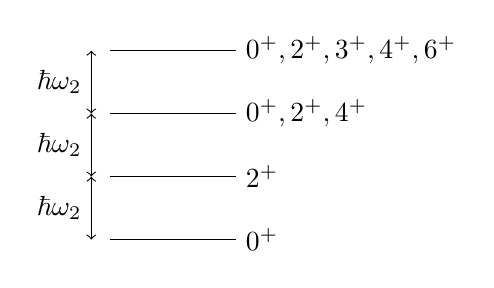
\begin{tikzpicture}[scale=0.8]
\draw (0,0) -- (2,0) node[right]{$0^+$};
\draw (0,1) -- (2,1) node[right]{$2^+$};
\draw (0,2) -- (2,2) node[right]{$0^+,2^+,4^+$};
\draw (0,3) -- (2,3) node[right]{$0^+,2^+,3^+,4^+,6^+$};
\foreach \y in {0,1,2} \draw[<->] (-0.3,\y) -- (-0.3,\y+1) node[midway,left]{$\hbar\omega_2$};
\end{tikzpicture}
\end{center}

\subsection{E2 transitions in the vibrational model}
Let us assume $E2$ transitions between the vibrational states ($0^+_2,2^+_2,4^+_1\xrightarrow{E2}2^+_1\xrightarrow{E2}0^+_1$; the operator $\alpha_{2\mu}$ does not connect $2^+_2\to0^+_1$ in the lowest order, and $M1$ transitions are absent), with
\[
B(XJ,J_i\to J_f)=\frac{\big|\braket{f\|\op{\mathcal M}^X_J\|i}\big|^2}{2J_i+1},\qquad
\braket{f|\op{\mathcal M}^X_{JM}|i}=\frac{1}{\sqrt{2J_f+1}}\big(J_iM_i\,JM\big|J_fM_f\big)\braket{f\|\op{\mathcal M}^X_J\|i},
\]
$\ket i=\ket{J_iM_i}$, $\ket f=\ket{J_fM_f}$. In the long-wave limit the transition operator is
\[
\op{\mathcal M}^E_{JM}=\sum_{i=1}^Ae^{(i)}r_i^J\,Y_{JM}(\vartheta_i,\varphi_i)
\]
\[
\text{or}\qquad\op{\mathcal M}^E_{JM}=\int\rho(\vec r)\,r^J\,Y_{JM}(\vartheta,\varphi)\,\ud^3r,\quad
\rho(\vec r)=\sum_{i=1}^Ae^{(i)}\delta(\vec r-\vec r_i).
\]
For constant $\rho$, $J=2$, and $R=R_0\big(1+\sum_\mu\alpha^*_{2\mu}Y_{2\mu}\big)$:
\[
\op{\mathcal M}^E_{2M}=\rho\int\ud^3r\,r^2Y_{2M}(\Omega)=\rho\int\ud\Omega\,Y_{2M}(\Omega)\int_0^{R(\Omega)}\ud r\,r^4
=\frac\rho5\int\ud\Omega\,Y_{2M}(\Omega)\,R^5(\Omega)
\]
\[
\approx\frac\rho5R_0^5\int\ud\Omega\,Y_{2M}(\Omega)\Big(1+5\sum_\mu\alpha_{2\mu}Y^*_{2\mu}+10\sum_{\mu\mu'}\alpha_{2\mu}\alpha_{2\mu'}Y^*_{2\mu}Y^*_{2\mu'}+\dots\Big)
\approx\rho R_0^5\,\alpha_{2M},
\]
i.e.\ $\op{\mathcal M}^E_{2M}\sim\alpha_{2M}$. One can add higher-order terms:
\[
\Rightarrow\quad \op{\mathcal M}^E_{2M}=\rho R_0^5\Big(\alpha_{2M}-\sqrt{\frac{10}{7\pi}}\big[\alpha_2\times\alpha_2\big]^2_M\Big)+\dots
\]
To the lowest order the transition operator is $\op{\mathcal M}^E_{2\mu}=\rho R_0^5\,\op\alpha_{2\mu}$ with
\[
\op\alpha_{2\mu}=\frac12\sqrt{\frac{2\hbar}{B_2\omega_2}}\Big(\op\beta^\dagger_{2\mu}+(-1)^\mu\op\beta_{2-\mu}\Big).
\]
We see that the term $\sim\op\alpha_{2\mu}$ can connect only states which differ by 1 phonon, whereas the higher terms also give contributions to transitions between states which differ by more phonons.
\[
B(E2,2^+_1\to0^+_1)=\frac{\big|\braket{0^+_1\|\op{\mathcal M}^E_2\|2^+_1}\big|^2}{5},
\qquad
\braket{0^+_1\,0|\op{\mathcal M}^E_{20}|2^+_1\,0}=\big(20\,20\big|00\big)\braket{0^+_1\|\op{\mathcal M}^E_2\|2^+_1},
\]
\[
\braket{0^+_1\|\op{\mathcal M}^E_2\|2^+_1}=\frac{1}{\underbrace{(20\,20|00)}_{1/\sqrt5}}\Big\langle0^+_1\,0\Big|\rho R_0^5\,\frac12\sqrt{\frac{2\hbar}{B_2\omega_2}}\,\op\beta_{20}\op\beta^\dagger_{20}\Big|0\Big\rangle ,
\]
\[
B(E2,2^+_1\to0^+_1)=\rho^2R_0^{10}\,\frac{\hbar}{2\underbrace{B_2\omega_2}_{\sqrt{B_2C_2}}}
=\Big(\frac{3Ze}{4\pi}R_0^2\Big)^2\frac{\hbar}{2\sqrt{B_2C_2}},
\qquad \rho=\frac{Ze}{\frac43\pi R_0^3}=\frac{3Ze}{4\pi R_0^3},\quad \omega_2=\sqrt{\frac{C_2}{B_2}} .
\]
We can fix the parameters $C_2$, $B_2$ from the experimental $B(E2,2^+_1\to0^+_1)$ and $E_{2^+_1}\equiv\hbar\omega_2=\hbar\sqrt{C_2/B_2}$.
One can show
\[
\boxed{B(E2;\,0^+_2,2^+_2,4^+_1\to2^+_1)=2\,B(E2;\,2^+_1\to0^+_1)},
\]
i.e.\ the transitions from the two-phonon triplet are $2\times$ stronger:
\begin{center}
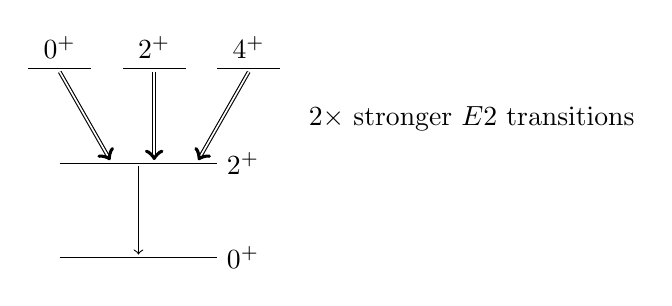
\begin{tikzpicture}[scale=0.8]
\draw (0,3) -- (1,3) node[above,pos=0.5]{$0^+$};
\draw (1.5,3) -- (2.5,3) node[above,pos=0.5]{$2^+$};
\draw (3,3) -- (4,3) node[above,pos=0.5]{$4^+$};
\draw (0.5,1.5) -- (3,1.5) node[right]{$2^+$};
\draw (0.5,0) -- (3,0) node[right]{$0^+$};
\draw[->,double] (0.5,2.95) -- (1.3,1.55);
\draw[->,double] (2,2.95) -- (2,1.55);
\draw[->,double] (3.5,2.95) -- (2.7,1.55);
\draw[->] (1.75,1.45) -- (1.75,0.05);
\node[right] at (4.3,2.2) {$2\times$ stronger $E2$ transitions};
\end{tikzpicture}
\end{center}
\paragraph{Note:} with $\beta_0^2=\frac{5\hbar}{2B_2\omega_2}$ (the mean square deformation in the ground state) we have $B(E2,2^+_1\to0^+_1)\sim\beta_0^2$.

%=====================================================================
\section{Rotational motion of deformed nuclei}
\label{sec:rot}
%=====================================================================
As we gradually move away from systems with closed shells, a deformed shape becomes energetically more favoured over the spherical one. Experimentally we find that well-deformed nuclei have unfilled shells both in protons and neutrons.

A simple phenomenological quantity correlated with the onset of deformation can be defined:
\[
P=\frac{N_pN_n}{N_p+N_n},
\]
where $N_p$, $N_n$ are the numbers of valence protons and neutrons, respectively. We see that it is proportional to the number of $p$--$n$ valence pairs. It turns out that for $P\gtrsim4$--5 we clearly see spectra which are typical for well-deformed nuclei, namely
\[
E_{4^+_1}/E_{2^+_1}\doteq3.33 .
\]

\subsection{Collective Hamiltonian in the intrinsic frame}
Let us discuss now how one can describe the large variety of collective states in deformed even-even nuclei in terms of the collective model. We start again from the quadrupole degrees of freedom, which can be described via $\alpha_{2\mu}$:
\[
R(\vartheta,\varphi)=R_0\Big[1+\sum_{\mu=0,\pm1,\pm2}\alpha^*_{2\mu}Y_{2\mu}(\vartheta,\varphi)\Big].
\]
$\alpha_{2\mu}$ transform under rotations like spherical tensors: for $\vartheta,\varphi\xrightarrow{\ \mathcal R\ }\vartheta',\varphi'$
\[
\alpha'_{\lambda\mu}=\sum_\nu D^\lambda_{\nu\mu}\,\alpha_{\lambda\nu},
\]
where $D^\lambda_{\nu\mu}(\vartheta_1,\vartheta_2,\vartheta_3)$ is the Wigner $D$ function and the rotation is parametrized by the Euler angles $\vartheta_1,\vartheta_2,\vartheta_3$. This allows us to construct invariants
\[
\big[\alpha_2\times\alpha_2\big]^0=\sum_\mu\big(2\mu\,2\,{-\mu}\big|00\big)\alpha_{2\mu}\alpha_{2-\mu},\qquad
\Big[\big[\alpha_2\times\alpha_2\big]^2\times\alpha_2\Big]^0,\ \dots
\]
One can define a system (intrinsic frame) in which
\[
\alpha'_{2\pm2}\neq0,\qquad \alpha'_{2\pm1}=0,\qquad \alpha'_{20}\neq0,
\]
i.e.\ nonzero values only for $\alpha'_{2\pm2}$, $\alpha'_{20}$:
\[
\alpha'_{2\pm2}\equiv a_2=\frac{1}{\sqrt2}\beta\sin\gamma,\qquad \alpha'_{20}\equiv a_0=\beta\cos\gamma .
\]
They are usually parametrized by the Bohr variables $\beta,\gamma$: $\beta$ --- quadrupole deformation parameter, $\gamma$ --- triaxiality. So instead of $\alpha_{2\mu}$ we can use $\beta,\gamma$ $+$ $\vartheta_1,\vartheta_2,\vartheta_3$ as collective variables.

One can then derive the Hamiltonian describing the collective motion. For the Hamiltonian
\[
H=\sum_\mu\frac{B_2}{2}|\dot\alpha_{2\mu}|^2+V(\alpha_{2\mu})
\]
it is reasonable to assume that $V$ depends \underline{only} on the deformation parameters $\beta,\gamma$ and not on the orientation given by $\vartheta_1,\vartheta_2,\vartheta_3$. The derivation of the kinetic-energy part is lengthy, but one can get the result
\[
H=T+V,\qquad
T=T_{\rm rot}+\frac12B_2\big(\dot\beta^2+\beta^2\dot\gamma^2\big),\qquad
T_{\rm rot}=\frac12\sum_{k=1}^3\mathcal J_k\,\omega_k^2 ,
\]
where $\mathcal J_k$ are the components of the moment of inertia in the body-fixed (rotating) frame and $\omega_k$ are the components of the angular velocity around the body-fixed axes (in which the moment of inertia is diagonal with elements $\mathcal J_k$). $T_{\rm rot}$ is the collective rotational energy.

If $\beta$ and $\gamma$ are not constant, rotational and vibrational motion are coupled in a complicated way, since $\mathcal J_k$ are functions of $\beta,\gamma$. One can derive the values for an irrotational liquid and for a rigid body; the experimental values $\mathcal J^{\rm exp}$ satisfy
\[
\mathcal J^{\rm irrot}<\mathcal J^{\rm exp}<\mathcal J^{\rm rigid}.
\]

\subsection{Quantized collective (Bohr) Hamiltonian}
Further, one has to quantize the Hamiltonian ($\beta,\gamma,\vartheta_1,\vartheta_2,\vartheta_3\to$ operators). The result is
\[
\op H=-\frac{\hbar^2}{2B_2}\Big[\frac{1}{\beta^4}\frac{\partial}{\partial\beta}\Big(\beta^4\frac{\partial}{\partial\beta}\Big)
+\frac{1}{\beta^2\sin3\gamma}\frac{\partial}{\partial\gamma}\Big(\sin3\gamma\frac{\partial}{\partial\gamma}\Big)\Big]
+\op T_{\rm rot}+V(\beta,\gamma),
\]
\[
\op T_{\rm rot}=\frac{\op I'^2_1}{2\mathcal J_1}+\frac{\op I'^2_2}{2\mathcal J_2}+\frac{\op I'^2_3}{2\mathcal J_3},
\]
where $\op I'_i$ are the angular momentum projections onto the body-fixed axes.

Note that $\op T_{\rm rot}$ can be guessed from the classical expression for the rotational energy
\[
T_{\rm rot}=\frac12\sum_{ij}\omega_i\omega_j\mathcal J_{ij}=\frac12\vec\omega^{\,T}\mathcal J\,\vec\omega .
\]
In the body-fixed frame
\[
\mathcal J=\begin{pmatrix}\mathcal J_1&&\\&\mathcal J_2&\\&&\mathcal J_3\end{pmatrix},\qquad
\vec I=\mathcal J\vec\omega,\qquad \vec\omega=\mathcal J^{-1}\vec I,\qquad
\mathcal J^{-1}=\begin{pmatrix}1/\mathcal J_1&&\\&1/\mathcal J_2&\\&&1/\mathcal J_3\end{pmatrix},
\]
\[
T_{\rm rot}=\frac12\big(\mathcal J^{-1}\vec I\big)^T\mathcal J\big(\mathcal J^{-1}\vec I\big)
=\frac12\vec I^{\,T}\mathcal J^{-1}\mathcal J\mathcal J^{-1}\vec I
=\frac12\vec I^{\,T}\mathcal J^{-1}\vec I
=\frac12\Big(\frac{I'^2_1}{\mathcal J_1}+\frac{I'^2_2}{\mathcal J_2}+\frac{I'^2_3}{\mathcal J_3}\Big).
\]

\subsection{Axially symmetric rigid rotor}
Let us discuss the case of an axially symmetric rigid rotor (symmetry axis 3): $\gamma=0$, $\beta\equiv\beta_0$, $\mathcal J_1=\mathcal J_2\equiv\mathcal J$, and the system does not rotate around the symmetry axis.
\[
\op T_{\rm rot}\equiv\op H_{\rm rot}=\frac12\Big(\frac{\op I'^2_1+\op I'^2_2}{\mathcal J}\Big)+\frac12\frac{\op I'^2_3}{\mathcal J_3}
=\frac12\Big(\frac{\op{\vec I}'^2}{\mathcal J}+\Big(\frac{1}{\mathcal J_3}-\frac1{\mathcal J}\Big)\op I'^2_3\Big),
\]
where $\op{\vec I}'^2=\op{\vec I}^2$ is invariant.
One can find the explicit expression of $\op I'_i$ in terms of $(\vartheta_1,\vartheta_2,\vartheta_3)$ and find the eigenvalues and eigenstates of $\op H_{\rm rot}$:
\[
\op H_{\rm rot}\ket{MKI}=E_{\rm rot}\ket{MKI},\qquad
\op{\vec I}^2\ket{MKI}=\hbar^2I(I+1)\ket{MKI},
\]
\[
\op I_3\ket{MKI}=\hbar M\ket{MKI},\qquad
\op I'_3\ket{MKI}=\hbar K\ket{MKI},
\]
\[
E_{\rm rot}=\frac{\hbar^2}{2}\Big[\frac{I(I+1)}{\mathcal J}+\Big(\frac{1}{\mathcal J_3}-\frac1{\mathcal J}\Big)K^2\Big],
\]
where $M$ is the projection of the angular momentum onto the laboratory $z$ axis and $K$ the projection onto the body-fixed $z'$ axis.
\begin{center}
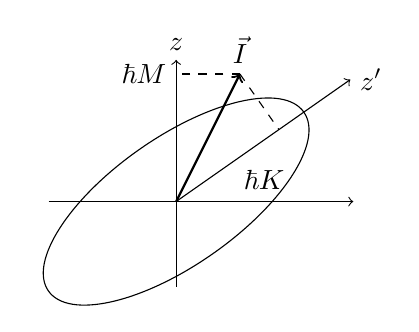
\begin{tikzpicture}[scale=0.9]
\draw[->] (-1.8,0) -- (2.5,0);
\draw[->] (0,-1.2) -- (0,2.0) node[above]{$z$};
\draw[rotate=35] (0,0) ellipse (2.2 and 0.9);
\draw[->] (0,0) -- (35:3.0) node[right]{$z'$};
\draw[->,thick] (0,0) -- (0.9,1.8) node[above]{$\vec I$};
\draw[dashed] (0.9,1.8) -- (0,1.8) node[left]{$\hbar M$};
\draw[dashed] (0.9,1.8) -- ($(35:{0.9*cos(35)+1.8*sin(35)})$);
\node at (35:1.0) [below right] {$\hbar K$};
\end{tikzpicture}
\end{center}
From the expression for $E_{\rm rot}$ we see that for each $K$ we have $E_{\rm rot}\sim I(I+1)$ $\to$ \textbf{rotational band}.
For the ground state of even-even nuclei $I_{\rm g.s.}=0^+$ $\Rightarrow$ $K=0$ $\Rightarrow$ ground-state band.
Moreover, the wave function has a symmetry with respect to rotation around any axis perpendicular to $z'$.
\begin{center}
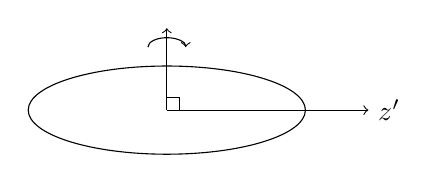
\begin{tikzpicture}[scale=0.8]
\draw (0,0) ellipse (2.2 and 0.7);
\draw[->] (0,0) -- (3.2,0) node[right]{$z'$};
\draw[->] (0,0) -- (0,1.3);
\draw[->] (-0.3,1.0) arc (180:0:0.3 and 0.15);
\draw (0,0.2) -- (0.2,0.2) -- (0.2,0);
\end{tikzpicture}
\end{center}
One can show that this leads to wave functions of the form
\[
\sim\Big[\ket{IMK}+(-1)^I\ket{IM\,{-K}}\Big]
\]
$\Rightarrow$ for $K=0$ only even $I$ are allowed $\Rightarrow$ the ground-state band of even-even well-deformed nuclei:
\begin{center}
\begin{tikzpicture}[scale=0.8]
\draw (0,0) -- (2,0) node[right]{$0^+$};
\draw (0,0.6) -- (2,0.6) node[right]{$2^+$};
\draw (0,2.0) -- (2,2.0) node[right]{$4^+$};
\draw (0,4.2) -- (2,4.2) node[right]{$6^+$};
\end{tikzpicture}
\end{center}
\[
E_{\rm rot}=\frac{\hbar^2}{2}\,\frac{I(I+1)}{\mathcal J},\qquad
\frac{E(4^+)}{E(2^+)}=\frac{4\cdot5}{2\cdot3}\doteq3.33 .
\]
It turns out that in the representation of Euler angles
\[
\braket{\vartheta_1\vartheta_2\vartheta_3|IMK}\equiv\phi_{IMK}=N\,D^{I*}_{MK}(\vartheta_1,\vartheta_2,\vartheta_3),
\]
with the Wigner rotation matrices
\[
D^I_{MK}(\vartheta_1,\vartheta_2,\vartheta_3)=\braket{IM|\op{\mathcal R}(\vartheta_1,\vartheta_2,\vartheta_3)|IK},
\]
\[
\op{\mathcal R}(\vartheta_1,\vartheta_2,\vartheta_3)=\op{\mathcal R}_z(\vartheta_1)\op{\mathcal R}_y(\vartheta_2)\op{\mathcal R}_z(\vartheta_3)
=\op{\mathcal R}_{z'}(\vartheta_3)\op{\mathcal R}_{y'}(\vartheta_2)\op{\mathcal R}_z(\vartheta_1),
\]
\[
D^I_{MK}(\vartheta_1,\vartheta_2,\vartheta_3)=\braket{IM|e^{-i\vartheta_1\op I_3}e^{-i\vartheta_2\op I_2}e^{-i\vartheta_3\op I_3}|IK}.
\]
The Wigner $D$ functions fulfil
\[
\int_0^{2\pi}\ud\vartheta_3\int_0^\pi\ud\vartheta_2\sin\vartheta_2\int_0^{2\pi}\ud\vartheta_1\;D^{I*}_{MK}\,D^{I'}_{M'K'}=\frac{8\pi^2}{2I+1}\,\delta_{II'}\delta_{MM'}\delta_{KK'} .
\]

\subsection{E2 transitions and quadrupole moments in rotational bands}
The knowledge of the collective wave function allows us to calculate the strong intraband transitions ($I+2\xrightarrow{E2}I\to\dots$). One can show that within the band
\[
B(E2,I_i\to I_f)=\frac{\big|\braket{I_fM_fK\|\op{\mathcal M}^{\rm el}_2\|I_iM_iK}\big|^2}{2I_i+1}.
\]
For a well-deformed axially symmetric quadrupole shape with deformation $\beta$
\[
B(E2,I_i\to I_f)=\Big(\frac{3ZeR_0^2}{4\pi}\Big)^2\beta^2\,\big(I_iK\,20\big|I_fK\big)^2
\]
is proportional to $\beta^2$ $\Rightarrow$ this is how we can extract $|\beta|$ from the intensities of $E2$ transitions.

Moreover, we can relate the intrinsic quadrupole moment and the laboratory one. For a quadrupole shape, the intrinsic quadrupole moment is
\[
Q_0=\sqrt{\frac{16\pi}{5}}\,\frac{3}{4\pi}\,ZeR_0^2\,\beta,
\]
where $R_0$ is the radius of the corresponding sphere, and
\[
B(E2,I_i\to I_f)=\frac{5}{16\pi}\,Q_0^2\,\big(I_iK\,20\big|I_fK\big)^2 .
\]
In order to measure the sign of $Q_0$ we need to measure the spectroscopic quadrupole moment
\[
Q_{IMK}\equiv\braket{IMK|\op Q_{33}|IMK},\qquad Q_{\rm lab}\equiv\braket{IIK|\op Q_{33}|IIK}.
\]
One can easily derive
\[
\underbrace{Q_{IIK}}_{\text{laboratory}}=\underbrace{Q_0}_{\text{intrinsic}}\,\frac{3K^2-I(I+1)}{(I+1)(2I+3)} .
\]
We can measure $Q_{IIK}\to Q_0\to\beta$ --- the ``experimental'' quadrupole deformation.
Note that for $K=0$, $I=0$: $Q_{IIK}=0$ $\Rightarrow$ we have to measure it for excited states of even-even nuclei.

%=====================================================================
\subsection{Rotational-vibrational spectrum}
%=====================================================================
Let us start again from the collective Bohr Hamiltonian
\[
\op H=-\frac{\hbar^2}{2B_2}\Big[\frac{1}{\beta^4}\frac{\partial}{\partial\beta}\Big(\beta^4\frac{\partial}{\partial\beta}\Big)
+\frac{1}{\beta^2\sin3\gamma}\frac{\partial}{\partial\gamma}\Big(\sin3\gamma\frac{\partial}{\partial\gamma}\Big)\Big]
+\sum_{i=1}^3\frac{\op I'^2_i}{2\mathcal J_i}+V(\beta,\gamma),
\]
with the irrotational moments of inertia
\[
\mathcal J_i=4B_2\beta^2\sin^2\Big(\gamma-\frac{2\pi i}{3}\Big),\qquad i=1,2,3 .
\]
For a deep minimum at the deformation $\beta=\beta_0$ and $\gamma=0^\circ$, corresponding to an axially symmetric ground-state deformation, we can simplify the Hamiltonian:
\begin{center}
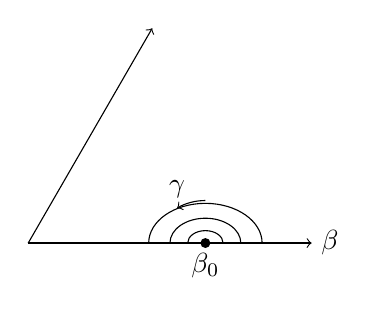
\begin{tikzpicture}[scale=0.9]
\draw[->] (0,0) -- (4,0) node[right]{$\beta$};
\draw[->] (0,0) -- (60:3.5);
\foreach \r in {0.25,0.5,0.8} \draw (2.5+\r,0) arc (0:180:\r cm and 0.7*\r cm);
\fill (2.5,0) circle (2pt) node[below]{$\beta_0$};
\draw[->] (2.5,0.6) arc (90:120:0.8) node[above]{$\gamma$};
\end{tikzpicture}
\end{center}
\begin{enumerate}
\item Moments of inertia:
\[
\mathcal J_1(\beta,\gamma)=\mathcal J_2(\beta,\gamma)\approx\mathcal J_1(\beta_0,0)=\mathcal J_2(\beta_0,0)\equiv\mathcal J_0,
\]
\[
\mathcal J_0=4B_2\beta_0^2\underbrace{\sin^2\Big(-\frac{2\pi}{3}\Big)}_{3/4}=4B_2\beta_0^2\sin^2\Big(-\frac{4\pi}{3}\Big)=3B_2\beta_0^2,
\]
\[
\mathcal J_3=4B_2\beta_0^2\underbrace{\sin^2(\gamma-2\pi)}_{\approx\gamma^2}\approx4B_2\beta_0^2\gamma^2 .
\]
\item Potential:
\[
V(\beta,\gamma)\approx V(\beta_0,0)+C_\beta(\beta-\beta_0)^2+C_\gamma(\gamma-\underbrace{\gamma_0}_{0})^2
=V(\beta_0,0)+\frac12B_2\omega_\beta^2(\beta-\beta_0)^2+\frac12B_2\beta_0^2\omega_\gamma^2\gamma^2 .
\]
\end{enumerate}
Then
\[
\op H\approx\underbrace{-\frac{\hbar^2}{2B_2}\frac{\partial^2}{\partial\beta^2}+\frac12B_2\omega_\beta^2(\beta-\beta_0)^2}_{\op H_\beta}
\]
\[
\qquad\ \underbrace{-\frac{\hbar^2}{2B_2\beta_0^2}\,\frac1\gamma\frac{\partial}{\partial\gamma}\gamma\frac{\partial}{\partial\gamma}+\frac{\op I'^2_3}{8B_2\beta_0^2\gamma^2}+\frac12B_2\beta_0^2\omega_\gamma^2\gamma^2}_{\op H_\gamma}
\]
\[
\qquad\ +\underbrace{\frac{\op{\vec I}^{\,2}-\op I'^2_3}{6B_2\beta_0^2}}_{\op H_{\rm rot}}+\underbrace{V(\beta_0,0)}_{\rm const},
\]
\[
\op H\approx\op H_\beta+\op H_\gamma+\op H_{\rm rot}
\]
$\Rightarrow$ we can find a factorized solution
\[
\ket{\Psi_{n_\beta n_\gamma IMK}}=\ket{\varphi_{n_\beta}}\ket{\xi_{n_\gamma K}}\ket{\phi_{IMK}} .
\]
We see that $\op H_\beta$ describes harmonic vibrations in $\beta$. One can show that $\op H_\gamma$ corresponds to a 2-dimensional HO in polar coordinates $(r,\varphi)\to(\gamma,2\vartheta_3)$, where $\vartheta_3$ is an Euler angle. $\op H_{\rm rot}$ is an axially symmetric rotor. The energy is given by
\[
E_{n_\beta n_\gamma IK}=\hbar\omega_\beta\Big(n_\beta+\frac12\Big)+\hbar\omega_\gamma\underbrace{\Big(2n_\gamma+1+\frac{|K|}{2}\Big)}_{N_\gamma+1}+\frac{\hbar^2}{2\mathcal J_0}\big[I(I+1)-K^2\big],
\qquad N_\gamma=2n_\gamma+\frac12|K|,
\]
\[
n_\beta=0,1,2,\dots,\qquad n_\gamma=0,1,2,\dots,\qquad K=0,2,4,\dots
\]
\[
\ket{\Psi_{n_\beta n_\gamma IMK}}=\underbrace{\ket{\varphi_{n_\beta}}\ket{\xi_{n_\gamma K}}}_{\substack{\text{intrinsic (vibrational) part}\\ \text{depending on }\beta,\gamma}}\ \underbrace{\ket{\phi_{IMK}}}_{\substack{\text{rotational part}\\ \sim D^{I*}_{MK}(\vec\vartheta)}} .
\]
The spectrum $\Rightarrow$ rotational bands superimposed on vibrational band-heads ($K=0,2,4,\dots$, $n_\beta=0,1,2,\dots$, $n_\gamma=0,1,2,\dots$):
\begin{center}
\begin{tikzpicture}[xscale=2.3,yscale=0.6]
% a = hbar^2/2J0 (scaled), band head energies: g.s. 0, gamma: 1*w_g, beta: w_b, ...
\def\a{0.12}
\def\wg{3.0}
\def\wb{4.2}
\newcommand{\band}[5]{% x, head energy, K, list of I, label
  \foreach \I in {#4} {
    \pgfmathsetmacro{\E}{#2+\a*(\I*(\I+1)-#3*#3)}
    \draw (#1,\E) -- (#1+0.6,\E) node[right,font=\scriptsize]{$\I^+$};
  }
  \node[below,align=center,font=\scriptsize] at (#1+0.3,-0.4) {#5};
}
\band{0}{0}{0}{0,2,4,6}{g.s.\ band\\$K=0$}
\band{1.1}{\wg}{2}{2,3,4,5}{$\gamma$ band\\$K=2$, $n_\gamma=0$\\$\hbar\omega_\gamma$}
\band{2.2}{\wb}{0}{0,2,4}{$\beta$ band\\$n_\beta=1$, $K=0$\\$\hbar\omega_\beta$}
\band{3.3}{2*\wg}{4}{4,5,6}{2nd $\gamma$ band\\$K=4$, $n_\gamma=0$\\$2\hbar\omega_\gamma$}
\band{4.4}{2*\wg}{0}{0,2,4,6}{3rd $\gamma$ band\\$n_\gamma=1$, $K=0$\\$2\hbar\omega_\gamma$}
\band{5.5}{2*\wb}{0}{0,2,4}{2nd $\beta$ band\\$n_\beta=2$, $K=0$\\$2\hbar\omega_\beta$}
\end{tikzpicture}
\end{center}
(The figure is schematic; the vertical scale is arbitrary.)

$\beta$ and $\gamma$ bands are observed in many well-deformed nuclei.

\end{document}
